\documentclass[a4paper,12pt]{book}

% Paquetes necesarios
\usepackage[utf8]{inputenc}   % Codificación de caracteres
\usepackage[spanish]{babel}   % Idioma español
\usepackage[T1]{fontenc}      % Codificación de fuentes
\usepackage{amsmath, amssymb} % Símbolos matemáticos
\usepackage{graphicx}         % Inclusión de gráficos
\usepackage{cite}             % Gestión de citas
\usepackage{hyperref}         % Enlaces y referencias
\usepackage{geometry}         % Configuración de márgenes
\usepackage{fancyhdr}         % Encabezados y pies de página
\usepackage{titlesec}         % Formato de títulos
\usepackage{booktabs}         % Tablas profesionales
\usepackage{caption}          % Personalización de leyendas
\usepackage{enumitem}         % Personalización de listas
\usepackage{float}
\usepackage{tcolorbox}
\usepackage[table]{xcolor} % Paquete para colores en tablas
\usepackage{colortbl}       % Complemento para colorear celdas específicas
\usepackage{multirow}       % Combinar celdas en tablas
\usepackage{makecell}       % Combinar celdas en tablas
\usepackage{enumitem}
\usepackage{amsmath}
\usepackage{eurosym}
\usepackage{tikz}
\usepackage{listings}
\usepackage{color}
\usepackage{float}
\usepackage{pdfpages}

%\newcommand{\micode}[1]{\lstinline[basicstyle=\ttfamily, keywordstyle=\bfseries, breaklines=true]{#1}}      % Cargar el paquete listings
\lstdefinelanguage{Dockerfile}{
    morekeywords={FROM, RUN, CMD, LABEL, MAINTAINER, EXPOSE, ENV, ADD, COPY, ENTRYPOINT, VOLUME, USER, WORKDIR, ARG, ONBUILD, STOPSIGNAL, HEALTHCHECK, SHELL},
    sensitive=true,
    morecomment=[l]{\#},
    morestring=[b]"
}

% Define YAML language for listings
\lstdefinelanguage{yaml}{
  keywords={true,false,null,y,n},
  keywordstyle=\color{blue}\bfseries,
  basicstyle=\ttfamily,
  sensitive=false,
  comment=[l]{\#},
  morecomment=[s]{/*}{*/},
  commentstyle=\color{gray}\ttfamily,
  stringstyle=\color{red}\ttfamily,
  morestring=[b]',
  morestring=[b]"
}
% Configuración para que listings soporte UTF-8
\lstset{
    extendedchars=true,  % Permite caracteres extendidos (opcional en versiones recientes)
    inputencoding=utf8,  % Asegura que listings entienda UTF-8
    breaklines=true,
    emphstyle=\itshape,
    basicstyle=\ttfamily, keywordstyle=\bfseries,
    literate={á}{{\'a}}1 {é}{{\'e}}1 {í}{{\'i}}1 {ó}{{\'o}}1 {ú}{{\'u}}1 
             {Á}{{\'A}}1 {É}{{\'E}}1 {Í}{{\'I}}1 {Ó}{{\'O}}1 {Ú}{{\'U}}1
             {ñ}{{\~n}}1 {Ñ}{{\~N}}1 {¿}{{¿}}1 {¡}{{¡}}1
}

% Definir \micode con soporte para tildes
\newcommand{\micode}[1]{\lstinline{#1}}

%creacion de un lstlisting claro y bonito
\lstdefinestyle{mystyle}{
    backgroundcolor=\color{white},   
    commentstyle=\color{green},
    keywordstyle=\color{blue},
    numberstyle=\tiny\color{gray},
    stringstyle=\color{red},
    basicstyle=\ttfamily\footnotesize,
    breakatwhitespace=false,         
    breaklines=true,                 
    captionpos=b,                    
    keepspaces=true,                 
    numbers=left,                    
    numbersep=5pt,                  
    showspaces=false,                
    showstringspaces=false,
    showtabs=false,                  
    tabsize=2
}

\lstdefinestyle{yamlstyle}{
    backgroundcolor=\color{yellow!10},   
    commentstyle=\color{purple},
    keywordstyle=\color{orange},
    numberstyle=\tiny\color{blue},
    stringstyle=\color{teal},
    basicstyle=\ttfamily\footnotesize\bfseries,
    breakatwhitespace=false,         
    breaklines=true,                 
    captionpos=b,                    
    keepspaces=true,                 
    numbers=left,                    
    numbersep=5pt,                  
    showspaces=false,                
    showstringspaces=false,
    showtabs=false,                  
    tabsize=2,
    morekeywords={true,false,null,y,n}
}

\lstdefinestyle{directorystructure}{
    backgroundcolor=\color{gray!10},   
    commentstyle=\color{green!50!black},
    keywordstyle=\color{blue!70},
    numberstyle=\tiny\color{gray},
    stringstyle=\color{red!70!black},
    basicstyle=\ttfamily\footnotesize,
    breakatwhitespace=false,         
    breaklines=true,                 
    captionpos=b,                    
    keepspaces=true,                 
    numbers=none,                    
    showspaces=false,                
    showstringspaces=false,
    showtabs=false,                  
    tabsize=2
}

\lstnewenvironment{directorylisting}[1][]{
    \lstset{
        style=directorystructure,
        caption={#1},
        frame=single,
        framerule=0.5pt,
        rulecolor=\color{black!50},
        xleftmargin=0.5cm,
        xrightmargin=0.5cm
    }
}{}



\setlength{\headheight}{14.5pt}

% Configuración de márgenes
\geometry{left=3cm, right=3cm, top=2.5cm, bottom=2.5cm}

% Configuración de encabezados y pies de página
% \setlength{\headheight}{14.49998pt}
\pagestyle{fancy}
\fancyhf{}
\fancyhead[L]{Universidad de Granada}
\fancyhead[L]{\nouppercase{\leftmark}}

% \fancyhead[C]{Escuela Técnica Superior de Ingenierías Informática}
\fancyhead[R]{Ingeniería de Servidores}
\fancyfoot[L]{\rule[0pt]{\textwidth}{0.2pt}\\Ismael Sallami Moreno}
\fancyfoot[C]{\rule[0pt]{\textwidth}{0.2pt}\\\thepage}
\fancyfoot[R]{\rule[0pt]{\textwidth}{0.2pt}\\\today}
\renewcommand{\sectionmark}[1]{\markboth{#1}{}} % Configura \leftmark para que solo muestre la sección

\lstdefinestyle{customstyle}{
    backgroundcolor=\color{gray!10},   
    commentstyle=\color{green!50!black}\itshape,
    keywordstyle=\color{blue!70}\itshape,
    numberstyle=\tiny\color{gray}\itshape,
    stringstyle=\color{red!70!black}\itshape,
    basicstyle=\ttfamily\footnotesize\itshape,
    breakatwhitespace=false,         
    breaklines=true,                 
    captionpos=b,                    
    keepspaces=true,                 
    numbers=left,                    
    numbersep=5pt,                  
    showspaces=false,                
    showstringspaces=false,
    showtabs=false,                  
    tabsize=2,
    frame=single,
    framerule=0.5pt,
    rulecolor=\color{black!50},
    xleftmargin=0.5cm,
    xrightmargin=0.5cm,
    literate={á}{{\'a}}1 {é}{{\'e}}1 {í}{{\'i}}1 {ó}{{\'o}}1 {ú}{{\'u}}1 
             {Á}{{\'A}}1 {É}{{\'E}}1 {Í}{{\'I}}1 {Ó}{{\'O}}1 {Ú}{{\'U}}1
             {ñ}{{\~n}}1 {Ñ}{{\~N}}1 {¿}{{¿}}1 {¡}{{¡}}1
}

\lstnewenvironment{customlisting}[1][]{
    \lstset{
        style=customstyle,
        caption={#1}
    }
}{}


% Formato de títulos
\titleformat{\section}{\large\bfseries}{\thesection.}{0.5em}{}
\titleformat{\subsection}{\normalsize\bfseries}{\thesubsection.}{0.5em}{}

% Datos del documento
\title{\textbf{Prácticas Ingeniería de Servidores}}
\author{
    Ismael Sallami Moreno \\
    \texttt{ism350zsallami@correo.ugr.es}
}
\date{
    \vspace{1cm}
    \begin{tabular}{rl}
        \textbf{Asignatura:} & Ingeniería de Servidores \\
        \textbf{Tema:} & Prácticas \\
        \textbf{Fecha:} & \today
    \end{tabular}
}

\begin{document}

% Portada
\begin{titlepage}
    \begin{center}
        % \vspace*{1cm}
        
        % \Huge
        % \textbf{Práctica Contabilidad Financiera II}
        \Huge \textbf{Prácticas Ingeniería de Servidores} 
        % \vspace{0.5cm}
        % \LARGE
        % \textbf{Ismael Sallami Moreno}\\
        % \LARGE
        % \texttt{ism350zsallami@correo.ugr.es}
        % \LARGE
        % \url{https://github.com/Ismael-Sallami}
        
        % \vfill
        
        % \Large
        % \textbf{Universidad de Granada}
        
        \vspace{0.8cm}
        
        \begin{tikzpicture}[remember picture, overlay]
            \node[opacity=0.2] at (current page.center) {
\includegraphics[width=\paperwidth,height=\paperheight]{portada.jpg}};
            \node[align=center] at (current page.center) {
                
                \vspace{0.5cm}
                \LARGE \textbf{Ismael Sallami Moreno} \\
                \LARGE \texttt{ism350zsallami@correo.ugr.es} \\
                \LARGE \url{https://ismael-sallami.github.io/} \\
                \LARGE \url{https://elblogdeismael.github.io/} \\
                \vspace{2cm}
                \Large \textbf{Universidad de Granada} \\
                \vspace{0.8cm}
                % \Large \textbf{2025}
            };
        \end{tikzpicture}
        \vfill
        
        \Large
        \textbf{2025}
        
    \end{center}
\end{titlepage}
\newpage


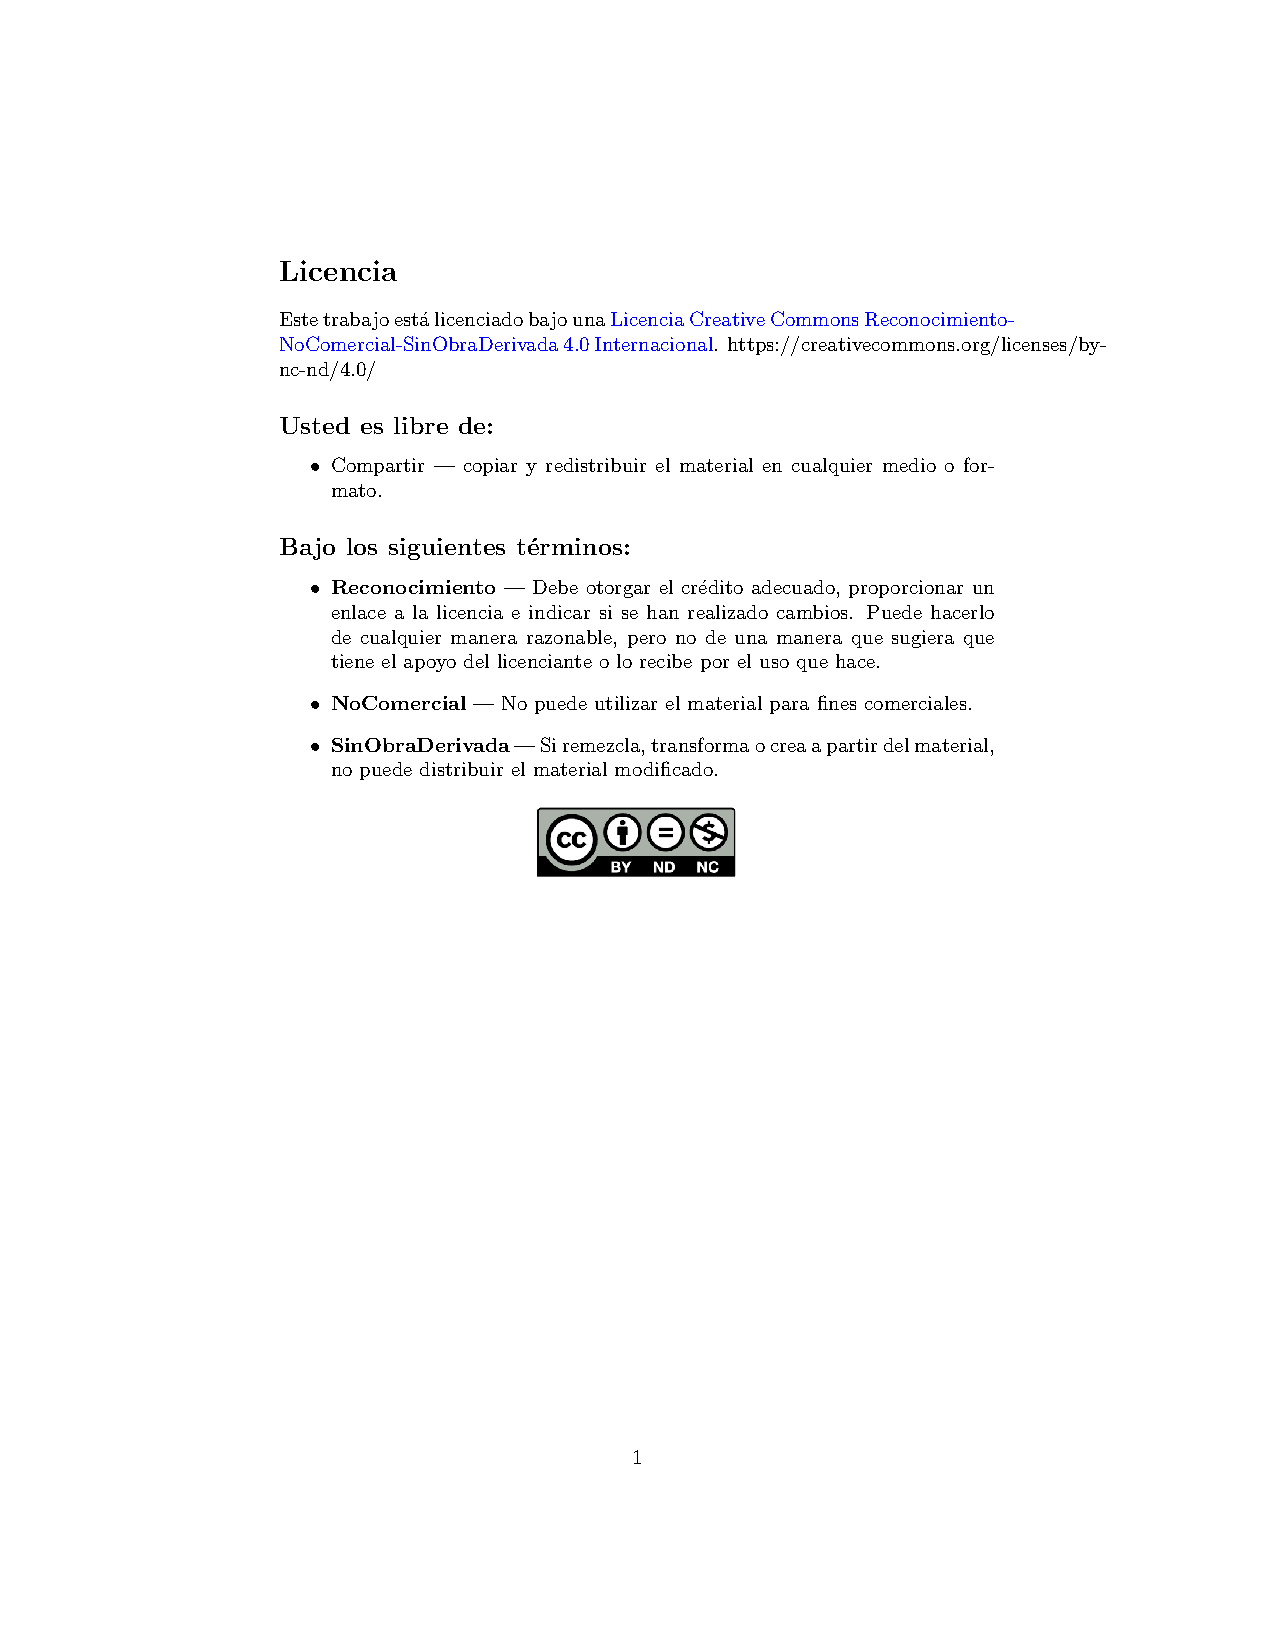
\includepdf[pages=-]{../../../../../../extraFiles/licencia.pdf}
% Tabla de contenidos
\tableofcontents
\newpage

\part{Apuntes de Clase}

\chapter{Bloque 1}

\section{Ping y SSH}

Sobre esta parte no decidí tomar apuntes en clase debido a que son conceptos vistos en la Asignatura de Fundamentos de Redes, por lo que consideré que no era necesario. De todas formas en la parte de Prácticas (Resolución) se comenta paso a paso lo que se hizo en esta parte.
\newpage
\section{LVM y RAID}

\subsection{LVM (Logical Volume Manager)}

\begin{itemize}
    \item \textbf{Discos y particiones}:
    \begin{itemize}
        \item \micode{sda}: Primer disco del sistema.
        \item Luego pueden existir \micode{sdb}, \micode{sdc}, etc.
    \end{itemize}
    \item Consideraciones importantes:
    \begin{itemize}
        \item Si el directorio \micode{/boot} se llena, el sistema podría fallar al arrancar debido a la falta de espacio disponible.
        \item Se recomienda evitar el uso de \micode{swap} en sistemas virtualizados, ya que reduce el rendimiento.
    \end{itemize}
\end{itemize}

\subsection{Directorios base en Linux}
\begin{itemize}
    \item \textbf{/boot}: Contiene los archivos de arranque del sistema.
    \item \textbf{/etc}: Almacena los archivos de configuración del sistema operativo.
    \item \textbf{/dev}: Contiene archivos especiales que representan dispositivos del sistema.
    \item \textbf{/mnt}: Punto de montaje temporal para sistemas de archivos.
    \item \textbf{/var}: Contiene datos variables del sistema, como logs y archivos temporales. Puede crecer mucho, por lo que se recomienda monitorearlo.
\end{itemize}

\subsection{RAID (Redundant Array of Independent Disks)}

RAID es una tecnología que permite combinar múltiples discos para mejorar la redundancia y/o el rendimiento del sistema de almacenamiento.

\subsection{Ventajas}
\begin{itemize}
    \item Permite unir volúmenes de almacenamiento.
    \item Mejora el rendimiento si los discos están en buses distintos, ya que permite acceso en paralelo.
\end{itemize}

\subsection{Niveles de RAID}
\begin{itemize}
    \item \textbf{RAID 0 (Striping)}:
    \begin{itemize}
        \item Divide los datos en bloques y los distribuye entre varios discos.
        \item \textbf{Problema}: Si un disco falla, se pierde toda la información.
        \item Se usa poco en la práctica debido a su baja robustez.
    \end{itemize}
    
    \item \textbf{RAID 1 (Mirroring)}:
    \begin{itemize}
        \item Duplica los datos en dos o más discos.
        \item Si un disco falla, el otro sigue funcionando con los mismos datos.
        \item Aporta robustez al sistema.
        \item \textbf{Problema}: Se paga el doble en almacenamiento.
        \item Se usa frecuentemente en \micode{/boot} para garantizar que el sistema pueda arrancar en caso de fallo de un disco.
    \end{itemize}
    
    \item \textbf{RAID 5 (Paridad distribuida)}:
    \begin{itemize}
        \item Se distribuyen los datos y la paridad entre todos los discos.
        \item Si un disco falla, se pueden recuperar los datos utilizando la paridad.
        \item \textbf{Problema}: Puede reducir el rendimiento debido al tiempo necesario para calcular la paridad.
        \item \textbf{Ventaja}: Equilibra costos, robustez y capacidad de recuperación.
        \item Se puede usar un disco de repuesto que entra en acción si uno falla.
    \end{itemize}
\end{itemize}

\subsection{Tipos de RAID}
\begin{itemize}
    \item \textbf{RAID por Hardware}: 
    \begin{itemize}
        \item Utiliza un controlador RAID físico.
        \item Es más eficiente y transparente para el sistema operativo.
    \end{itemize}
    
    \item \textbf{RAID por Software}: 
    \begin{itemize}
        \item Administrado por el sistema operativo.
        \item Puede ser modificado por el administrador, lo que representa un riesgo.
        \item Requiere más recursos del sistema.
    \end{itemize}
\end{itemize}

\subsection{Ejercicio Opcional: Configuración de RAID1 para /var}

\subsection{Objetivo}
El objetivo es proporcionar a \micode{/var} un respaldo frente a fallos mediante la creación de un RAID1. Para ello, debemos montar un RAID1 y mover \micode{/var} dentro de este.

\subsection{Pasos a seguir}
\begin{enumerate}
    \item \textbf{Creación de discos virtuales en la máquina virtual (MV)}
    \begin{itemize}
        \item Se crean dos discos: \micode{raid1} y \micode{raid2}.
        \item Usamos \micode{lsblk} para verificar la existencia de \micode{sdb} y \micode{sdc}.
    \end{itemize}

    \item \textbf{Instalación de \micode{mdadm}}
    \begin{itemize}
        \item \micode{sudo dnf provides mdadm} (para verificar qué paquete lo proporciona).
        \item \micode{sudo dnf install mdadm} (para instalarlo).
    \end{itemize}

    \item \textbf{Creación del RAID1}
    \begin{itemize}
        \item \micode{sudo mdadm --create /dev/md0 --level=1 --raid-devices=2 /dev/sdb /dev/sdc}
        \item Aparecerá un \textit{warning} sobre la creación de metadatos, confirmamos con "sí".
        \item Para monitorear la sincronización del RAID:  
              \micode{watch -n 1 more /proc/mdstat}
        \item Luego, verificamos con \micode{lsblk}.
    \end{itemize}

    \item \textbf{Prueba de fallo de disco}
    \begin{itemize}
        \item Podemos simular la falla de un disco con:  
              \micode{echo 1 > /dev/sdb}
        \item Se observa que \micode{md0} sigue funcionando al ser un \textit{mirror}.
    \end{itemize}
\end{enumerate}

\subsection{LVM (Logical Volume Manager)}

\subsection{Conceptos Clave}
\begin{itemize}
    \item \textbf{LV (Logical Volume)}
    \item \textbf{VG (Volume Group)}
    \item \textbf{PV (Physical Volume)}
\end{itemize}

La estructura básica de LVM es la siguiente:

\begin{verbatim}
    LV         LV   
    '           '
   Volumen Group  
       '
   '     '     '
  pv    pv    pv  
\end{verbatim}

Un \textbf{Logical Volume (LV)} puede expandirse tomando espacio libre de otros discos o estructuras.

\subsection{Visualización de LVM}
\begin{itemize}
    \item Para ver los discos que son de tipo LVM, usamos \micode{lsblk} en la columna de \textit{type}.
    \item Para ver opciones de \micode{pv}, \micode{vg} y \micode{lv}, usamos \micode{tab-completion}.
\end{itemize}

\subsection{Consideraciones sobre Volumen Groups}
Si un \textbf{Volume Group} contiene un disco magnético, un SSD y un RAID, el acceso a los datos puede no ser homogéneo. Por ello, el volumen lógico debe montarse sobre el RAID.

\subsection{Creación del LVM sobre el RAID}
\begin{enumerate}
    \item Convertir el RAID en un Physical Volume:
          \micode{pvcreate /dev/md0}
    \item Crear un Volume Group llamado \micode{raid1}:
          \micode{vgcreate raid1 /dev/md0}
    \item Crear un Logical Volume de 10GB dentro del Volume Group:
          \micode{lvcreate -L 10G -n rvar raid1}
\end{enumerate}

\subsection{Movimiento de /var al RAID}
Después de crear el volumen lógico, debemos mover \micode{/var} dentro del RAID:

\begin{itemize}
    \item El nombre del volumen dentro del RAID es \micode{/dev/raid1/rvar}.
    \item También puede aparecer como \micode{/dev/mapper/raid1-rvar}, ya que son sinónimos creados mediante enlaces simbólicos.
\end{itemize}

\subsection{Resolución de Problemas}

\subsection{Problema 1: Configurar el sistema de archivos en \micode{rvar}}

Actualmente, el volumen lógico \micode{rvar} está vacío y sin un sistema de archivos. Para solucionarlo, seguimos estos pasos:

\begin{enumerate}
    \item \textbf{Seleccionar un sistema de archivos:}  
    Los sistemas de archivos recomendados son \textbf{ext4} y \textbf{xfs}, ya que son transaccionales y previenen la corrupción de datos en caso de fallos.  
    \item \textbf{Verificar los sistemas de archivos soportados:}  
    Ejecutamos el siguiente comando para listar los sistemas disponibles en el kernel:
    \begin{verbatim}
    ls /lib/modules/$(uname -r)/kernel/fs
    \end{verbatim}
    \item \textbf{Formatear el volumen lógico con \micode{ext4}:}
    \begin{verbatim}
    mkfs.ext4 /dev/mapper/raid1-rvar
    \end{verbatim}
\end{enumerate}

\subsection{Problema 2: Montar y trasladar /var al nuevo volumen}

El volumen lógico \micode{rvar} debe ser montado en el sistema y debemos trasladar \micode{/var} sin perder datos. Para ello:

\begin{enumerate}
    \item \textbf{Montar el volumen lógico:}  
    Primero, montamos \micode{rvar} en un directorio temporal:
    \begin{verbatim}
    mount /dev/mapper/raid1-rvar /mnt/
    \end{verbatim}
    Podemos verificar con:
    \begin{verbatim}
    mount
    \end{verbatim}
    Al revisar \micode{/mnt/}, aparecerá el directorio \micode{lost+found}, indicando que el sistema de archivos está activo.

    \item \textbf{Cambiar a modo mantenimiento:}  
    Para evitar la pérdida de datos al copiar \micode{/var}, debemos entrar en el \textbf{runlevel1}, también conocido como \textbf{modo mantenimiento}. Esto se hace con:
    \begin{verbatim}
    systemctl isolate runlevel1.target
    \end{verbatim}
    Podemos confirmar el estado con:
    \begin{verbatim}
    systemctl status
    \end{verbatim}

    \item \textbf{Copiar los datos de /var a /mnt/}:  
    Copiamos todo el contenido de \micode{/var} manteniendo atributos con:
    \begin{verbatim}
    cp -a /var/* /mnt/
    \end{verbatim}

    \item \textbf{Crear un respaldo de /var:}  
    Antes de reemplazar \micode{/var}, hacemos una copia de seguridad por si algo falla:
    \begin{verbatim}
    mv /var /var_old
    \end{verbatim}

    \item \textbf{Desmontar /mnt y montar el nuevo /var:}  
    \begin{verbatim}
    umount /mnt
    mkdir /var
    mount /dev/mapper/raid1-rvar /var
    \end{verbatim}
    Podemos verificar con:
    \begin{verbatim}
    df -h
    \end{verbatim}

    \item \textbf{Hacer el montaje permanente en \micode{/etc/fstab}:}  
    Si reiniciamos ahora, la configuración se perdería. Para evitarlo, editamos el archivo \micode{/etc/fstab} y agregamos la siguiente línea:
    \begin{verbatim}
    /dev/mapper/raid1-rvar      /var       ext4     defaults     0 0
    \end{verbatim}
    
    \item \textbf{Probar la configuración antes de reiniciar:}  
    \begin{verbatim}
    mount -a
    systemctl daemon-reload
    mount
    \end{verbatim}
    Si todo está correcto, reiniciamos el sistema.
\end{enumerate}

\subsection{Interpretación de \micode{lsblk}}

El comando \micode{lsblk} nos permite visualizar la estructura de almacenamiento del sistema. Es importante identificar:

\begin{itemize}
    \item \textbf{Discos físicos y particiones}: Aparecen como \micode{sda}, \micode{sdb}, \micode{sdc}, etc.
    \item \textbf{Volúmenes lógicos}: Se muestran bajo \micode{/dev/mapper/}.
    \item \textbf{SR0}: Indica la unidad de CD-ROM.
\end{itemize}

\newpage
\section{Firewall + SSHD}

Ya sabemos de otras Asignaturas que un \textbf{firewall} es un sistema que controla el tráfico de red, permitiendo o bloqueando ciertas conexiones. En Linux, el firewall más común es \textbf{iptables}.

El comando que tenemos que aprender a gestionar es \micode{firewall-cmd}, tiene diversas opciones como status, state. Otra forma para ver si esta arrancado es \micode{systemctl status firewall}.

Otras opciones: \micode{firewall-cmd --list-all}, en este comando debemos de ver los filtros que estan definidos, en services podemos ver los servicios que están habilitados.

Con sudo firewall-cmd --add-service=http, cuando lo listo otra vez, se añade el puerto http en la opción services. Cuando se hace con firewall-cmd, se hace dinámica, por lo que si reiniciamos esto se pierde. Para que se quede debemos de ejecutar el comando \micode{sudo fire firewall-cmd --runtime-to-permanent}. De forma alternativa, podemos ejecuar primero la opción \micode{--permanent} y luego \micode{--add-port=443/http}, pero si lo listamos no lo lleva a memoria, no hay ninguna opción que lo deje permanente y que lo lleve a memoria. Tenemos dos opciones o trabajar con servicios o llevarlo a memoria.

Si queremos conocer los servicios, podemos ejecutar \micode{firewall-cmd --get-services}.

Los firewalls en Linux son muy eficientes debido a que en este SO se trabaja con servicios, por lo que se puede controlar el tráfico de forma muy precisa. Al implementarse a nivel de Kernel ayuda a que sea muy eficiente.
\textit{No se va a preguntar nada sobre iptables}.

Debemos de usar el programa \micode{nmap} ya que nos dice que puertos están abietos en un servidor. Para instalarlo, usamos \micode{sudo dnf install nmap}. En el guión debemos de mirar la referenia número 31.

\subsection{Ejercicio Opcional}

Debemos de instalar un servicio HTTP, se recomienda Apache. Podemos escanear los 100 puertos mas usados con el comando \micode{nmap -F localhost}. Para instalar Apache, usamos \micode{sudo dnf install httpd}. Para arrancar el servicio, usamos \micode{sudo systemctl start httpd}. Para comprobar que está arrancado, usamos \micode{sudo systemctl status httpd}. Para que arranque en el inicio, usamos \micode{sudo systemctl enable httpd}. Para comprobar que está escuchando en el puerto 80, usamos \micode{sudo ss -tulnp | grep 80}.

Debemos de poder acceder desde el navegador de la máquina anfitrión.

\subsection{SSH}

Es un programa de terminal remoto, ya lo hemos usado en Asignaturas anteriormente. Antes se usaba Telnet, en este se especifica la dirección IP y el puerto, pero no era seguro, por lo que cualquier man in the middle podía interceptarlo y suplantar la identidad. Además, todas las respuestas que se producían eran en abierto, los \micode{cat},... En cambio, SSH es seguro, ya que se cifra la información. Este hace lo mismo que Telnet, pero de forma segura. Se recomienda hacerlo \micode{ssh usuario@ip}. O bien sustituir la IP por el nombre del dominio. Para cerrar la conexión, usamos \micode{exit}. 

Ya hemos estudiado en otras Asignaturas el tema de criptografía en cuanto al cifrado simétrico y asimétrico. En especial, en Fundamentos de Redes. Por si acaso, vamos a hacer una pequeña introducción. Tenemos dos tipos de cifrado:
\begin{itemize}
    \item \textbf{Cifrado simétrico}: Se usa una clave para cifrar y descifrar. El problema es que si alguien intercepta la clave, puede descifrar todo. Por ello, se usa poco.
    \item \textbf{Cifrado asimétrico}: Se usa una clave pública para cifrar y una privada para descifrar. La clave pública se puede compartir, pero la privada no. Se usa para firmar documentos, ya que si se cifra con la clave privada, solo se puede descifrar con la clave pública.
\end{itemize}

Debemos de destacar los conceptos de \textbf{autenticación} y \textbf{autorización}. La autenticación es el proceso de verificar la identidad de un usuario, mientras que la autorización es el proceso de verificar si un usuario tiene permiso para acceder a un recurso. Además, del uso de certificados digitales, que son un tipo de credencial que se usa para autenticar la identidad de un usuario o un servidor. Este se consigue a través de una entidad certificadora, usando una clave pública y privada (Big Brother).

Algoritmos :
\begin{itemize}
    \item Llave simétrica: DES(tenemos dos llaves, una que es privada y otra que es pública, lo que se cifra con la privada solo se puede descifrar con la pública, por dentro se gestiona en base a números primos muy grandes).
    \item Llave asimétrica: RSA (Se guarda la privada, mientras que la pública se comparte, estando incluso compartida en la propia web, de manera que la persona que quiera compartir contigo usa la pública para codificar el texto y te lo manda codificado, de esta manera si hay un man in the middle lo ve cifrado, solo la persona con la llave privada puede ver su contenido).
\end{itemize}

Otro uso de la llave privada es la \textit{firma}, de esta manera se garantiza la confidencialidad y la autenticación del mensaje debido a que es confidencial debido a que solo se puede descifrar con la llave pública, y autenticidad debido a que solo se puede cifrar con la llave privada, la cual solo conoce esa entidad.

Firma Digital: Usando Hash SHA256, se cifra con la llave privada y se envía el mensaje cifrado y el mensaje en abierto. La persona que recibe el mensaje cifrado con la llave privada, lo descifra y lo compara con el mensaje en abierto, si son iguales, se garantiza la autenticidad del mensaje. Ejemplo de ello puede ser el minado de monedas como es el Bitcoin. Además, otro ejemplo de ello es cuando descargamos algo y podemos verificar que es el del propio distribuidor usando el Hash que me proporciona. \textit{Por ende, podemos cosiderar que un HASH + llave privada es el certificado digital}. Para asegurarnos de que la llave pública es de quien dice ser debemos de ver el certificado digital, como hemos mencionado anteriormente. Este proceso para cuando encontramos un certificado digital que es de confianza, ya que si no lo es, no podemos asegurar que la llave pública sea de quien dice ser. Para ver los certificados, vemos que en Firefox, accedemos a settings y buscamos \textit{certificados}, podemos ver las entidades que nuestro browser reconoce.

\begin{tcolorbox}[colback=yellow!10!white, colframe=red!75!black, title=Advertencia]
El tema de certificados y demás al ser materia de Fundamentos de Redes, no se va a preguntar en el examen.
\end{tcolorbox}

Nos conectamos a un ordenador remoto mediante ssh, de esta manera le decimos que nos queremos conectar, el te envía la llave pública, es decir, se va a su configuración, recupera la llave y te la envía. A continuación, le enviamos nuestras creedenciales cifradas con la llave pública, y cuando le llega, las descifra con la llave privada y comprueba si son correctas. Si lo son, nos deja entrar. Si no lo son, nos dice que no podemos entrar. Además, de esta manera se prevee que un \textit{man-in-the-middle} no pueda interceptar las credenciales.

Podemos meterle una entrada en el fichero de host, de esta manera cuando nos conectamos a un servidor, nos conectamos a una IP, pero si le metemos una entrada en el fichero de host, le decimos que esa IP es un nombre, de esta manera cuando nos conectamos a ese nombre, nos conectamos a esa IP. Para ello, debemos de editar el fichero \micode{/etc/hosts} y añadir la IP y el nombre del servidor, así es más cómdo, para ello en Linux es \micode{ssh usuario@nombre}. 

Cuando ejecutamos el comando para conectarnos, nos imprime un mensaje con el HASH, y nos pregunta que si nos lo creemos, si en vez de una llave pública esta reconocida en nuestras llaves y ve que tenemos el certificado no nos preguntaría. En todos lo equipos se crea el directorio ssh en home, dentro de este tenemos un archivo que se llama known\_hosts, el cual contiene las llaves públicas de los ordenadores que ya has confiado, de manera que no nos va a preguntar cuando nos conectemos de nuevo, si queremos que en la primera vez tampoco pregunta la copiamos y pegamos, entre otras opciones. \textit{Nota: Por defecto se crea ese directorio cuando se conetca por ssh.}

Este proceso es muy costos en términos de cómputo, por lo que se usa lo más mínimo posible. Por esto se usa un proceso de handshaking, de esta manera el equipo le manda una propuesta de llave simétrica y de esta manera ya se usa en adelante, ya que el uso de clave privada y pública es muy costoso.

¿Cómo puedo acceder sin contraseña? Para ello nos autenticamos con llave pública y llave privada. En el caso de que decidamos hacerlo asi cuando le mandamos que soy 'nombre', recupera la llave de el directorio .ssh y le manda un mensaje de firmame esto con la clave privada de dicho usuario, y de esta manera se asegura de que efectivamente es el usuario que dice ser. Además, en el directorio home solo puede escribir el usuario y el root.

En la MV:

\begin{itemize}
    \item ssh-keygen: crea la llave privada dentro de home, luego nos pregunta si queremos protegerla con contraseña, si no queremos, le damos a enter, \textit{pero siempre debe de hacerse.} Luego si nos vamos al directorio vemos dos documentos la llave privada y la pública. Si queremos que no nos pregunte siempre la contraseña, usamos el comando \micode{ssh-agent}, de esta manera el la escribe por ti, hasta que usamos el comando \micode{exit}, en este caso se olvida.
\end{itemize}

Para usar la pública:
\begin{itemize}
    \item Accedemos al directorio /home/.ssh 
    \item usamos el comando ssh-copy-id usuario@{ip/hostname} (copia mi identidad, se puede hacer con ctrl+c/v), y luego nos hace una prueba para que le demostremos que de verdad somos el usuario al que nos queremos conectar, para ello le mandamos la contraseña.
    \item Luego comprobamos que podemos entrar sin contraseña.
    \item En la máquina donde nos hemos conectado, vemos un fichero llamado \textit{id\_rsa.pub}, y si lo listamos debe de ser el mismo que la clave pública de la máquina inicial, desde la que nos conectamos a esta.
\end{itemize}

\textit{Nota: El directorio .ssh se crea en el home cuando es el cliente, mientras que en el servidor se crea en el /etc/ssh, también podemos crearlo nosotros a priori.}

Ahora podemos ejecuar un comando remoto, por ejemplo: \micode{ssh usuario@ip comando}, de esta manera se ejecuta el comando en la máquina remota. En este punto comienza la automatización de configuración remota. \textit{Ansible son scripts pero ejecutados de manera remota.} Además, podemos copiar archivos usando el comando scp (secure copy), de esta manera se copia el archivo de una máquina a otra. \textit{Nota: scp es un comando de ssh.} El comando es \micode{scp origen destino}, por ejemplo: \micode{scp /home/usuario/archivo usuario@ip:/home/usuario/}, de esta manera se copia el archivo de la máquina local a la remota. Si queremos copiar un directorio, usamos el comando \micode{scp -r origen destino}. Además podemos conectarnos mediante \textit{sftp} (secure file transfer protocol), de esta manera se conecta a la máquina remota y podemos copiar archivos de manera interactiva. \textit{Nota: sftp es un comando de ssh.} Para conectarnos, usamos el comando \micode{sftp usuario@ip}, y luego podemos usar los comandos \micode{put} y \micode{get} para copiar archivos de una máquina a otra.

\subsection{Ejercicio Opcional}

En el ejercicio debemos de dar acceso mediante ssh usando la llave pública y privada, debemos de modificar el puerto para conectarnos en vez del 22 para el ssh usar otro que sea mayor que el 1024, para ello podemos asegurarnos de que no estamos colisionando con un puerto conocido buscando en Innternet.

\begin{enumerate}
    \item Accedemos al contenido del demonio del ssh que se encuentra en /etc/ssh, una vez dentro nos pone el comando que debemos de ejecuar \micode{semanage...} (aparece en el fichero de ssh de la máquina Rocky), para que se apliquen los cambios debemos de reiniciar el servicio, para ello usamos el comando \micode{sudo systemctl restart sshd} o bien reiniciar la máquina.
    \item Además debemos de modificar el firewall para permitir ese puerto, para ello usamos el comando \micode{sudo firewall-cmd --add-port=puerto/tcp --permanent}, y luego reiniciamos el servicio con \micode{sudo systemctl restart firewalld}.
    \item Luego debemos de copiar la llave pública a la máquina remota, para ello usamos el comando \micode{ssh-copy-id usuario@ip}, y luego nos pide la contraseña, una vez introducida, ya podemos conectarnos sin contraseña.
    \item Para comprobar que todo está correcto, usamos el comando \micode{ssh usuario@ip -p puerto}, de esta manera nos conectamos a la máquina remota.
\end{enumerate}

Con el parámetro -p le especificamos el puerto al que nos queremos conectar, de esta manera nos conectamos al puerto que hemos especificado, ya que de manera predeterminada se conecta al puerto 22.

\section{Automatización con Ansible}

Por defecto Ansible ya viene instalado en la mayoría de las distribuciones de Linux. Además, por defecto al instalar Ansible se instala Python y SSH. Para instalarlo debemos de usar el comando \micode{sudo dnf install ansible}. Para comprobar que está instalado, usamos el comando \micode{ansible --version}, o bien mediante el comando \micode{sudo dnf list installed | grep -i ansible}. Además, podemos ver la documentación de Ansible en la página oficial de Ansible. Su configuración se encuentra en /etc/ansible, \textit{este solo se instala en el controlador ya que es desde donde se maneja.}

En la configuración de /etc/ansible, podemos cambiar varios parámetro, como es el caso del número de hebras que usa o número de procesos que se ejecutan de manera pararela, en este caso suele estar por defecto en 5 hebras.

En nuestro directorio base\footnote{Accedemos con el comando \micode{cd}.}, tenemos el archivo \micode{.ansible.cfg}, el cual podemos editar siendo los cambios aplicados de la misma manera que si lo hiciéramos en el archivo de configuración de /etc/ansible. Por defecto viene vacío, pero tiene un comando para generar la configuración por defecto, el cual es \micode{ansible-config dump}. Además, podemos ver la configuración de Ansible con el comando \micode{ansible-config list}.

En cuanto al formato que se usa en Ansible, cabe destacar que se establecen etiquetas, como puede ser \micode{web server}, de manera que cuando ejecutemos Ansible, podemos elegir esta etiqueta para que lo lance con lo que esté definido debajo de dicha etiqueta en el archivo de configuración.

Entramos en ansible con \micode{cd .ansible}, y debemos de definir etiquetas para entrar a los hosts que se definen en este archivo de configuración. En este archivo se definen los hosts. 

Una de las referencias importante es la guía sobre AD-HOC y la lista de todos los módulos que podemos ejecutar\footnote{Referencias 42 y 43 del guión.}. LOs módulos que vienen po defecto son los \textit{ansible.builtin}. El pinf de Ansible, actúa de manera distinta, lo que hace es que comprueba si se tiene acceso al servidor al que se hace el ping y comprueba si este tiene pyhton instalado. Solo se le pasa un parámetro.

Para ejecutar un comando AD-HOC\footnote{Solo disponible en la controladora y no en las manejadas.} es con \micode{ansible ansi_control -m ping},este comando debe de darnos correcto si efectivamente puede ejecutar el comando de manera correcta. Cabe destacar que ansible\_control debe de estar en la configuración de ansible.
Otro de los comandos a destacar es: \micode{ansible ansible_control -m ping -a 'data = "Hola Mundo"'}, de nuevo \textbf{cabe destacar que el comando ansi\_control esta definido en la configuración de ansible}.

En clase estamos ejecutando comando con lo anteriormente mencionada, podemos destacar que si intentamos ejecutar comandos de sudo da error, para ello debemos de añadir \micode{--become}, pero nos pide la contraseña, esto no nos interesa ya que no queremos que nos pida la contraseña todas las máquinas.

Para ello nos vamos al fichero /etc/ y ejecutamos \micode{more sudo}. en .ansible las frases con \% delante es un grupo, vemos una línea que nos lo permite para todos (todos los wheels), pero esto es \textit{una mala práctica.}

Así que en vez de eso, añadimos la línea \micode{david  ALL=(ALL)  NOPASSWD:ALL}, debo de salir y volver a entrar, porque puede recordar sesiones anteriores de sudo. En este punto si nos deja entrar usando \micode{--become} sin poner la contraseña.

Con el comando \micode{ansible ansible-inventory --graph} vemos las máquinas que tenemoso bien podemos ejecutar \micode{ansible ansible-inventory -i <ruta fichero > --graph}.

Para más información sobre Ansible, podemos visitar la documentación oficial en \url{https://docs.ansible.com}. Aquí encontraremos guías, referencias y ejemplos que nos ayudarán a entender y utilizar Ansible de manera efectiva.

O bien acceder a esta url: \url{https://docs.ansible.com/ansible/latest/index.html} y sobretodo a esta \url{https://docs.ansible.com/ansible/latest/reference_appendices/YAMLSyntax.html}.

Para ejecutar un archivo .yaml es \micode{ansible -playbook -i <ruta fichero> <archivos extra>}.

El fichero basics.yaml que se usa en clase como ejemplo es:
\begin{lstlisting}[style=yamlstyle]
servers:
  hosts:
    ansi_control:
      ansible_host: 192.168.56.101
      ansible_user: david
      ansible_port: 22232
    ansi01:
      ansible_host: 192.168.56.111
      ansible_user: admin
    ansi02:
      ansible_host: 192.168.56.112
      ansible_user: admin
  vars:
    ansible_port: 22

unlagged:
  hosts:
    ansi01:
    ansi02:
\end{lstlisting}

Debemos de consultar las claves especiales en la documentación. La forma de depurar es comentar todo e ir ejecutando líneas y descomentando.

Cabe la posibilidad de hacer playbooks parametrizables.

Uno parte de los playbooks que se usan en clase es:

\begin{lstlisting}[style=yamlstyle]
- name: Esta el usuario alguien ahí?
  ansible.builtin.shell:
    cmd: who
  register: who_results (guarda el resultado del comando who en la variable who_results)

- name: Print Connected
  ansible.builtin.debug:
    msg: "Connected list: {{ who_results.stdout }}"
\end{lstlisting}

Tenemos que entregar un directorio con los ficheros\footnote{Básicamente todos los que usemmos.}: \begin{itemize}
    \item basics.yaml 
    \item ejecutaPlaybook.sh
    \item hosts.yaml
    \item vars.yaml: variables.
\end{itemize}


\subsection{Ejercicio Obligatorio}

En cuanto al ejercicio que debemos de \textbf{entregar}, el cambio que debemos de hacer es en /etc/sshd/.conf, ahí cambiamos la línea de AccessRoot y lo ponemos con el atributo \textit{yes}.

Los pasos son\footnote{Todo es dentro del playbook.}:
\begin{enumerate}
    \item Crear un nuevo usuario llamado “admin” que pueda ejecutar comandos privilegiados sin contraseña. \textit{Añadir usuario en las tasks de ansible y lo añadimos a sudoers}.
    \item Dar acceso por SSH al usuario “admin” con llave pública. \textit{Debemos de enviar la llave pública, buscando un módulo de ansible que lo hace.}
    \item Crear el grupo “wheel” (si no existe) y permitir a sus miembros ejecutar sudo. \textit{Existe, porque usamos Rocky, ausumimos que no sabemos que máquina es.} Si ejecutamos el mismo comando varias veces con los mismos parámetros el resultado final siempre es el mismo.
    \item Añadir una lista variable de usuarios (se proporcionará un ejemplo con al menos dos), añadiéndolos al grupo “wheel” y concediéndoles acceso por SSH con llave pública. La sacamos en el directorio .ssh y en el fichero id\_pub.
    \item Deshabilitar el acceso por contraseña sobre SSH para el usuario root.
\end{enumerate}

Estos quedan con un usuario admin que puede ejecutar comandos privilegiados sin contraseña.

Con esto podemos pasar el 2º playbook.

Debemos de realizar el ejercicio correspondiente a la creación de la web e instalación del servidor web

Un ejercicio interesante para comenzar es con \micode{ansible ansi_control -a "poweroff" --become}, ya que solo se apaga si esta todo correcto.

Para depurarlo si lo rechaza, debemos de:
\begin{enumerate}
    \item Me conecto con ssh.
    \item Probamos haciendo \micode{poweroff} con ssh, entre otras opciones.
\end{enumerate}



\chapter{Bloque 2}

\section{Breve introducción a Docker y contenedores}

Lo que proporcionan los contenedores es un entorno seguro donde nuestra máquina puede correr prgramas.

Podemos lanzar \textit{namespace} y este nos lanza un entorno en el que nos manda a nuestra raíz, de manera que tenemos un filesystem para nosotros. De esta forma tenemos un filesystem aislado. Si ejecutamos \micode{ps -ax} vemos que no vemos los procesos de la máquina anfitriona.   

La idea principal de las redes en los contenedores es que s puedan comunicar entre sí.

En resumen, los contenedores nos dan un espacio aislado y virtualizado. Hay un poco de pérdida de las prestaciones cuando se ejecuta el servicio de red virtualizado, pero es muy poco. Lo mas importante es que el acceso a memoria, CPU, ... son las mismas.

La principal utilización de los contenedores es porque te ofrece un espacio de safe box, y un espacio importante que es el \textit{filesystem privado}. 

Cuando se ejecuta en otros espacios se arrastran todas las dependencias.

Se puede extraer tanto la arquitectura como el sistema operativo, dependencias y demás.

Si necesito un analizador de red, puedo instalarlo sobre un docker y de esta manera no me ensucia mi espacio de trabajo y cuando necesito espacio puedo borrarlo.

En el caso de linux, todos los dockers son sistemas más pequeños sobre linux, con lo básico para que arranque.

Las aplicaciones que ejecutamos en el docker deben de ser ajustadas para que se ejcuten, debido a que la tecnología de docker es diferente a la de la máquina anfitriona.

Debemos de adaptarlo para que pregunte al contenedor por el límtie de aplicaciones que pueden ejecutar, para que todo se ejecute de la manera correcta.

\subsubsection*{Instalación de Docker}

Estan desarrolladas para Linux, por lo que no se puede correr en tecnologías de Windows, si se puede con las extensiones de Linux para Windows.

Usamos la guía de CentOs para instalarlo en Rocky, debemos de jercicio Obligatorio. Monitorización con Grafana + Prometheus.tener cuidado con la guía ya que en el último paso, aparecen pasos opcionales para que el docker sea ejecutado sin ser root (privilegios de superusuario).

Podemos instalar el DockerDesktop para un uso más sencillo, pero no es recomendable para un uso profesional.

Se puede ejecuatar sobre MacOs pero usando una máquina virtual, lo cual no tiene mucho sentido.

Entramos en \micode{docker-hub.com}, y buscamos el contenedor de \micode{hello-world}, ya que es el inicial para ver que todo funciona correctamente. Para ello debemos de ejuctar el comando \micode{docker pull hello-world}. Si no indicamos el número de versión, se instala la latest(última versión).

Lo ejecutamos con el comando \micode{docker run hello-world}. Una vez que ejecutamos el comando, se descarga la imagen y se ejecuta el contenedor, mostrando un mensaje para ver que todo ha funcionado correctamente.

\textbf{Todos los ejercicios son opcionales}.

A continuación debemos de centrarnos en el punto de OpenBenchMarking, que es un benchmarking de docker.

El de \micode{blender} es muy utilizado por marcas más comerciales para la renderización de imágenes y vídeos.

Debemos de tener en cuenta siempre las dependencias que necesitamos para ejecutar el contenedor.

Hay una aplicicación que se llama \micode{Phoronix}, que es un benchmarking de docker, pero para el Departamento de ISE, estan pensando en que esta en desuso.

Así que vamos a trabajar con Phoronix en un contenedor para que sea más sencillo de instalar y de ejecutar.

En la guía si buscamos Phoronix, bajamos el de \micode{pts}. Para ello ejecutamos el comando \micode{docker pull phoronix/pts}.

Con el comando \micode{docker images} vemos que se ha descargado la imagen.

SI ejecutamos el comando \micode{docker run -it phoronix/pts} (usamos el comando -it para que se ejecute en el primer plano y os dé una shell interactiva). Con el comando \micode{system-info}, podemos ver las información de los cores, incluso de los que están el un contenedor.

Con el comando \micode{system-sensors}, podemos ver los sensores que el ordenador tiene de manera nativa.

El comando \micode{phoronix-test-suite}(no es que sea un comando es lo que se muestra en la shell cuando ejecutamos el comando anterior de run), y si de seguido añadimos list-available-tests, podemos ver los test que podemos ejecutar. Para más info podemos acceder a la web de docker y en el apartado de dcoumentación.





\subsection*{Apache Benchmark}

Sirve para servidores http. Usando el comando \micode{ab} nos sale la información sobre el mismo. Algunos de los parámetros pueden ser:
\begin{itemize}
    \item -n: Número de peticiones.
    \item -c: Número de conexiones concurrentes.
    \item ...
\end{itemize}

Si lo hacemos con la ugr, podemos ver que en las características que el docuemnto html de la web aparece con muy pocos bytes. Probamos a ejecutar \micode{curl -v http://www.ugr.es}. En específico, \micode{curl} se usa para hacer peticiones http y depurar las mismas. \textit{Debemos de aprender a usarla}.

Vemos que la web de la ugr esta sobre https, por lo que apache-benchmark no se ha dado cuenta, por lo que debemos de usar el comando \micode{ab -n 20 -c 4 https://www.ugr.es/} (debemos de incluir la barra del final) y vemos que en este caso los bytes del html es mucho mayor y es más realista (previamente hemos ejecutado el comando \micode{curl -v http://www.ugr.es/}).



\subsection*{Simulación de Carga con Jmeter}

Se menciona como una tecnología a conocer en las entrevistas de trabajo, por lo que es importante conocerla. 

Usa Java, por lo que podemos usarlo con la última versión de Java.

La lanzamos en 2º plano para que no consuma la consola. Para ello ejecutamos el comando \micode{jmeter &}.

\begin{enumerate}
    \item Añadimos un elemento de thread, que corresponde con las hebras que se van a lanzar de manera concurrente. Para ello pulsamos add y seleccionamos thread group. Añadimos un nombre, hay parámetros que son importatantes. \textit{Se recomienda poner el Jmeter en Inglés para que no haya problemas con los nombres de los elementos y para que las guías de ayuda no tengan errores}. 
    \item Dentro del grupo de hebras creamos un \textit{sample}. Una de las ventajas de Apache es la gran inmensidad de plugins que tiene.  Dentro de sample seleccionamos la \textit{carga de http}. Gracias a la opción de \textit{follow redirects} hace que se ejecute redirecciones de manera automática.
    \item Configuramos los parámetros, como es el prorocolo que vamos a usar, puerto, ...
    \item Añadimos un \textit{listener} para poder ver los resultados (View Results Tree).Para desactivar un elemento debemos de hacer clic derecho y seleccionar la ocpión ``disable''. Hay plugins para poder ver los resultados de manera más visual.
\end{enumerate}

Si queremos simular que se diriga a una página secundaria (ugr.es/centros), debemos de añadir el nombre de la página en el campo de \textit{path}.
Podemos configurar el elmento común de\textit{ HTTP defaults}.

Podemos usar variables de usuario.
Podemos cargar el archivo que nos da bien con la extensión .jtl y usamos jmeter o con un excel (ya que es un archivo en formato csv). 

En cuanto a la aplicación de jmeter, debemos de tener en cuenta que en el order que aparezcan los elementos es el orden en el que se van a ejecutar.

Dentro de /var/logs, tenemos el archivo que muestra los logs y tiene una línea por cada usuario.

El usar el \textit{not sampler} es la forma más habitual de hacerlo, ya que es la forma más sencilla de hacerlo.

\subsection*{Instalación de la aplicación para el test con JMeter}

La aplicación que utilizaremos para el ejercicio de prueba de carga se encuentra en el repositorio de GitHub: \url{https://github.com/davidPalomar-ugr/iseP4JMeter.git}. 

Puede clonar el repositorio utilizando GIT o descargarlo como un archivo comprimido. Una vez descargado, obtendrá un nuevo directorio llamado \texttt{iseP4JMeter}, al cual podrá acceder y levantar la aplicación con los siguientes comandos:

\begin{verbatim}
cd iseP4JMeter
docker compose up
\end{verbatim}

El servicio se lanza en primer plano mostrando los logs de ejecución de sus componentes (incluidas las llamadas HTTP), lo que puede ser muy útil para depurar incidencias. Si desea que el servicio continúe en segundo plano, puede ejecutar el comando con la opción \texttt{-d}:

\begin{verbatim}
docker compose up -d
\end{verbatim}

\subsection*{Detalles sobre el Dockerfile y Docker Compose}

El \texttt{Dockerfile} es el archivo donde se especifican todos los comandos necesarios para crear una imagen de Docker y las acciones que debe realizar sobre esta (como copiar archivos, instalar paquetes o modificar configuraciones). Desde un punto de vista abstracto, podríamos decir que es el \textit{playbook} que Docker aplica al levantar el contenedor.

En este caso, la aplicación sobre la que aplicaremos la carga consta de dos contenedores configurados con sus respectivos \texttt{Dockerfile}s:

\subsubsection*{Dockerfile de la aplicación (Node.js):}

\begin{verbatim}
FROM node:16.13.0-stretch
RUN mkdir -p /usr/src/app
COPY . /usr/src/app
EXPOSE 3000
WORKDIR /usr/src/app
RUN ["npm", "install"]
ENV NODE_ENV=production
CMD ["npm", "start"]
\end{verbatim}

En este archivo se especifica:
\begin{itemize}
    \item La imagen base (\texttt{node:16.13.0-stretch}), que incluye Node.js versión 16.13.0 y Debian Stretch como sistema operativo base.
    \item La creación de un directorio y la copia de los archivos del repositorio en el contenedor.
    \item La exposición del puerto 3000 para la aplicación.
    \item La instalación de las dependencias con \texttt{npm install}.
    \item La ejecución de la aplicación con \texttt{npm start}.
\end{itemize}

\subsubsection*{Dockerfile de la base de datos (MongoDB):}

\begin{verbatim}
FROM mongo:6
COPY ./scripts/* /tmp/
RUN chmod 755 /tmp/initializeMongoDB.sh
WORKDIR /tmp
CMD ./initializeMongoDB.sh
\end{verbatim}

En este archivo se especifica:
\begin{itemize}
    \item La imagen base (\texttt{mongo:6}).
    \item La copia de scripts al contenedor y la asignación de permisos de ejecución.
    \item La ejecución de un script para inicializar la base de datos.
\end{itemize}

\subsubsection*{Archivo \texttt{docker-compose.yml}:}

El archivo \texttt{docker-compose.yml} permite configurar varios contenedores para que trabajen juntos como un único servicio. Su contenido es el siguiente:

\begin{verbatim}
version: '2.0'
services:
  mongodb:
    image: mongo:6
    ports:
      - "27017:27017"
  mongodbinit:
    build: ./mongodb
    links:
      - mongodb
  nodejs:
    build: ./nodejs
    ports:
      - "3000:3000"
    links:
      - mongodb
\end{verbatim}

Este archivo define:
\begin{itemize}
    \item El servicio de MongoDB, exponiendo el puerto 27017.
    \item La inicialización de MongoDB con datos mediante un contenedor adicional.
    \item El servicio de la aplicación Node.js, exponiendo el puerto 3000 y enlazándolo con MongoDB.
\end{itemize}

Para más detalles, consulte la documentación oficial de Docker Compose.

\subsection*{Ejercicio Obligatorio: Simulación de Carga HTTP con JMeter}

El repositorio \url{https://github.com/davidPalomar-ugr/iseP4JMeter.git} contiene la aplicación objeto de la prueba de carga y una descripción de los requerimientos sobre la carga a simular. Siga las instrucciones del repositorio y elabore la prueba de carga con JMeter.

El ejercicio debe realizarse en un directorio que contenga todos los artefactos necesarios para la ejecución de la prueba de carga. Los \textit{paths} a los archivos deben definirse de forma relativa para garantizar que la ejecución sea independiente de la ubicación del directorio. 

Como validación final, debe ser capaz de ejecutar la prueba de carga desde la línea de comandos (sin interfaz gráfica) desde cualquier directorio de su equipo.

\textit{Dentro de la web donde se encuentra la información del ejercicio se nos va indicando lo que debemos de ir haciendo.}

Cuando usamos la API, debemos de tener cuidado con los espacios para evitar errores, además cada alumno solo puede consultar su propio expediente.

Nos vamos a donde hemos clonado el repositorio y ejecutamos el comando \micode{./pruebaEntorno.sh}. 

Para los carácteres extraños que no codifica adecuadamente las webs, podemos usar webs como \textit{urlencoder} para ver como sería codíficado, por ejemplo ``\_'' es ``\%40''

Cuando ejecutmos el comando anterior de \micode{./pruebaEntorno.sh}, se lista varios elementos como es el token que están separados mediante ``.''.

Usando webs como JWT Decoder, si copiamos y pegamos el token aquí, podemos ver la información que contiene. Si mantenemos el ratón en el tiempo de expiración, podemos ver la fecha y hora de expiración. 

Como no se proporciona seguridad, en términos de que cualquiera puede interceptar el token, se nos da un número que representa al usuario en vez del correo (el token si está firmado con la llave), es decir, no esta cifrado pero sí firmado, por ende, podemos ver si lo ha firmado una entidad de confianza.

En cuanto al uso de la herramienta aleatoria, lo relacionado con esto no será materia evaluable. 

\begin{enumerate}
  \item Debemos de crear en Jmeter:
  \begin{itemize}
    \item Thread Group.
    \item Alumnos.
    \begin{itemize}
      \item Dentro de este debemos de crear un HTTP Request y añadirle login y passwd (será de tipo ``POST''), en cuanto al valor que debemos de añadir es \${login} y \${passwd}.
      \item Creamos un \textit{CSV Data Set Config} para poder cargar los datos de los alumnos.
      \item Ahora añadimos un \micode{Post Prodesador}, y este solamente afecta al login.
      \item Luego, añadimos un archivo ``Extraer JWT''. Cuando editamos el archivo, debemos de añadir la variable correspondiente y el campo de valor pasarle el token: ``\${TOKEN}''.
    \end{itemize}
  \end{itemize}
  \item Creamos las variables que se indican con TestPlan.
\end{enumerate}
\textit{Básicamente debemos de leernos la documentación para poder realizar la práctica.}

Los documentos que debemos de tener según las clases de teoría son:

\begin{figure}[H]
  \centering
  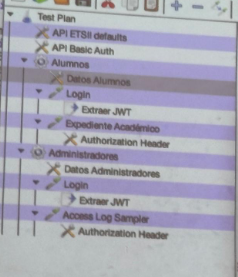
\includegraphics[width=0.8\textwidth]{images/Bloque2/docs_clase_jmeter.png}
  \caption{Documentos necesarios para la práctica.}
  \label{fig:documentos_practica}
\end{figure}

Debemos de entregar en Prado los archivos de carga ya que lo demás lo tiene él.

\subsection*{Docker Compose}

Docker Compose es una herramienta que permite definir y ejecutar aplicaciones Docker de múltiples contenedores. Con Compose, puedes usar un archivo YAML para configurar los servicios de tu aplicación, y luego con un solo comando puedes crear e iniciar todos los servicios desde esa configuración, este lee nuestro archivo \texttt{docker-compose.yml} y levanta los contenedores según la configuración especificada.

Entramos en \micode{hub.docker.com} y buscamos \micode{mongo:6} la imagen es un cuadrado\footnote{El link es \url{https://hub.docker.com/r/litmuschaos/mongo}.}. Ya solo queda entrar en el docker y ejecutar ese contenedor de manera independiente haciendo uso del comando \micode{docker run -it mongo:6}.

En el Docker Compose no necesitamos el mapeado de puertos. 

Si entramos en el directorio mongodb y abrimos el archivo dockerfile\footnote{Es similar a un makefile.} y lo ejecutamos, se nos crea un contenedor de mongo, vemos que ejecuta el archivo init.db, inicializando la base de datos con los datos que esten ahí definidos. Una imagen se basa en otra y así hasta que al final se llega a la imagen de linux.  


\section{Monitoring}

\subsection*{Top}

Para ejecutarlo en nuestra máquina debemos de ejecutar el comando \micode{top}. Este comando nos muestra los procesos que se están ejecutando en la máquina, junto con información sobre el uso de CPU, memoria y otros recursos.

Si ejecutamos el comando \micode{more loadavg}, nos ofrece en cada momentos el valor de los programas, tiempo de ejecución, etc.

El comando \micode{wath -n <tiempo> <"comando">}, de esta manera nos ejecuta el comando que se expone cada <tiempo> segundos.

Si vemos en una máquina con un solo core vemos un 1, quiere decir, que siempre había un proceso esperado para ejecutarse, es decir, que la CPU esta saturada, el uso de la CPU es del 200\%.

Si tenemos un 1 y 2 cores, significa que la CPU está al 50\%, es decir, que no está saturada.

Si tenemos 4 cores y tenemos un 4, significa que la CPU está al 100\%.

\subsection*{Información de Top en Linux}

El comando \texttt{top} en Linux muestra información en tiempo real sobre los procesos en ejecución y el estado del sistema. A continuación, se explica el significado de cada elemento que aparece en su salida:

\subsubsection*{Encabezado del sistema (primeras líneas)}

Este bloque muestra información general del sistema.

\paragraph{Primera línea: Tiempos de actividad}
\begin{verbatim}
top - 16:35:28 up 2:15,  2 users,  load average: 1.23, 0.85, 0.67
\end{verbatim}
\begin{itemize}
  \item \textbf{16:35:28}: Hora actual del sistema.
  \item \textbf{up 2:15}: Tiempo que el sistema lleva encendido (en este caso, 2 horas y 15 minutos).
  \item \textbf{2 users}: Número de usuarios conectados.
  \item \textbf{load average: 1.23, 0.85, 0.67}: Promedio de carga del sistema en los últimos 1, 5 y 15 minutos. Valores cercanos o superiores al número de núcleos indican alta carga.
\end{itemize}

\paragraph{Segunda línea: Tareas en ejecución}
\begin{verbatim}
Tasks: 180 total, 2 running, 177 sleeping, 1 stopped, 0 zombie
\end{verbatim}
\begin{itemize}
  \item \textbf{180 total}: Número total de procesos.
  \item \textbf{2 running}: Procesos que están ejecutándose activamente.
  \item \textbf{177 sleeping}: Procesos en espera de eventos.
  \item \textbf{1 stopped}: Procesos detenidos (pausados).
  \item \textbf{0 zombie}: Procesos "zombie" (terminados pero aún en la tabla de procesos).
\end{itemize}

\paragraph{Tercera línea: Uso de CPU}
\begin{verbatim}
%Cpu(s):  3.5 us,  1.2 sy,  0.0 ni, 95.0 id,  0.2 wa,  0.0 hi,  0.1 si,  0.0 st
\end{verbatim}
\begin{itemize}
  \item \textbf{us (user)}: \% de CPU utilizado por procesos de usuario.
  \item \textbf{sy (system)}: \% de CPU utilizado por procesos del sistema (kernel).
  \item \textbf{ni (nice)}: \% de CPU consumido por procesos con prioridad ajustada (\texttt{nice}).
  \item \textbf{id (idle)}: \% de CPU inactiva.
  \item \textbf{wa (I/O wait)}: \% de CPU esperando operaciones de entrada/salida (disco, red).
  \item \textbf{hi (hardware interrupts)}:\% de CPU manejando interrupciones de hardware.
  \item \textbf{si (software interrupts)}: \% de CPU manejando interrupciones de software.
  \item \textbf{st (steal time)}: \% de CPU "robado" por una máquina virtual (si se ejecuta en un entorno virtualizado).
\end{itemize}

\paragraph{Cuarta y quinta líneas: Uso de memoria RAM y Swap}
\begin{verbatim}
MiB Mem :   7854.2 total,   2364.5 free,   3184.8 used,   1304.9 buff/cache
MiB Swap:   2048.0 total,   1024.0 free,   1024.0 used.  2345.6 avail Mem
\end{verbatim}
\begin{itemize}
  \item \textbf{Mem total}: Memoria RAM total del sistema.
  \item \textbf{free}: Memoria libre disponible.
  \item \textbf{used}: Memoria en uso.
  \item \textbf{buff/cache}: Memoria usada como caché y buffers.
  \item \textbf{Swap total}: Tamaño total del área de intercambio (swap).
  \item \textbf{Swap free}: Espacio de swap no utilizado.
  \item \textbf{Swap used}: Espacio de swap en uso.
  \item \textbf{avail Mem}: Memoria disponible para nuevas aplicaciones.
\end{itemize}

\subsubsection*{Lista de procesos}

Esta sección muestra información sobre los procesos en ejecución. Cada columna tiene un significado:

\begin{verbatim}
PID   USER      PR  NI    VIRT    RES    SHR S  %CPU %MEM     TIME+ COMMAND
\end{verbatim}

\paragraph{Columnas principales}
\begin{itemize}
  \item \textbf{PID}: Identificador único del proceso.
  \item \textbf{USER}: Usuario que ejecuta el proceso.
  \item \textbf{PR (priority)}: Prioridad del proceso.
  \item \textbf{NI (nice)}: Valor \texttt{nice}, afecta la prioridad del proceso (-20 = más prioridad, 19 = menos prioridad).
  \item \textbf{VIRT (virtual memory)}: Memoria virtual utilizada (RAM + swap).
  \item \textbf{RES (resident memory)}: Memoria RAM utilizada sin contar swap.
  \item \textbf{SHR (shared memory)}: Memoria compartida con otros procesos.
  \item \textbf{S (state)}: Estado del proceso:
  \begin{itemize}
    \item \texttt{R}: Running (ejecutándose).
    \item \texttt{S}: Sleeping (durmiendo).
    \item \texttt{D}: Uninterruptible sleep (espera de I/O).
    \item \texttt{T}: Stopped (detenido).
    \item \texttt{Z}: Zombie (proceso finalizado, pero aún listado).
  \end{itemize}
  \item \textbf{\%CPU}: Porcentaje de uso de CPU del proceso.
  \item \textbf{\%MEM}: Porcentaje de uso de RAM del proceso.
  \item \textbf{TIME+}: Tiempo total de CPU consumido por el proceso.
  \item \textbf{COMMAND}: Comando o nombre del proceso.
\end{itemize}

\subsubsection*{Atajos útiles en \texttt{top}}

\begin{itemize}
  \item \texttt{q}: Salir de \texttt{top}.
  \item \texttt{h}: Mostrar ayuda.
  \item \texttt{k}: Matar un proceso (requiere PID).
  \item \texttt{M}: Ordenar por uso de memoria.
  \item \texttt{P}: Ordenar por uso de CPU.
  \item \texttt{T}: Ordenar por tiempo de ejecución.
\end{itemize}


Si entramos en el directorio /proc/sys/net/ipv4, podemos ver los parámetros de configuración del kernel.

Además del comando \micode{uptime}, podemos usar el comando free, que nos muestra la memoria libre y ocupada. Si usamos el comando \micode{free -h}, nos muestra la información en un formato más legible (human readable). Una de las ventajas de estos comandos es que no es interactivo, es decir, que ocupan la terminal, como si lo es el comando \micode{top}. Además, podemos usar el comando \micode{vmstat}.

El comando \micode{stress} se usa para generar pruebas artificiales sobre el uso de memoria y demás.

Si usamos \micode{htop}, es una versión mejorada de \micode{top} y nos muestra la información de una manera más visual. Para instalarlo, usamos el comando \micode{apt install htop}. Si lo ejecutamos, vemos que se nos muestra la información de una manera más visual.

\section{Cron}

Este se define como un demonio que se encarga de ejecutar tareas programadas en el sistema. Se utiliza para automatizar tareas repetitivas, como copias de seguridad, actualizaciones de software y mantenimiento del sistema. Podemos usar herramientas externas como \url{https://freeformatter.com}, para que nos de la configuración del crontab traduciendo para ello la expresión cron. Una alternativa a cron es \micode{anacron}. Este se ejecuta por defecto una vez cada hora.

Debemos de aprender a manejar el comando \micode{journalctl}. Si usamos \micode{journalctl -f}, nos muestra los logs en tiempo real. Si usamos \micode{journalctl -u cron}, nos muestra los logs del servicio de cron. Si usamos \micode{journalctl -u cron --since "2023-10-01 12:00:00"}, nos muestra los logs desde esa fecha y hora, tenemos una gran infinidad de opciones para filtrar los logs\footnote{Para ello podemos entrar en la documentación oficial.}. Cuando reiniciamos el equipo, perdemos los mensajes de logs de ayer, por lo que debemos de tener cuidado con esto. Para habilitarlo debemos de entrar en /etc/systemd/journald.conf y cambiar el parámetro de Storage de auto a yes, descomentando la línea. 

El programa \micode{logrotate} se encarga de gestionar los logs, y lo podemos encontrar en /etc/logrotate.conf. Este programa se encarga de rotar los logs, es decir, de crear un nuevo log y eliminar el antiguo. Si no lo tenemos configurado, los logs pueden ocupar mucho espacio en disco. Dentro de logrotate.d podemos añadir archivos de configuración para cada uno de los logs.


\section{Grafana + Prometheus}

Prometheus es el encargado de preguntarle a cada nodo por sus métricas, este proceso se llama \textbf{scraping}. Lo que almacena son series temporales mediante muestreos que realiza cada cierto tiempo. Puede presentar una interfaz de usuario, pero esta es muy pobre.

Una alternativa de usar la BD de Prometheus es \textit{InfluxDB} que es una opción de BD más rápida.

Vamos a usar la que tiene Grafana mediante en lenguaje de\textit{ PromQL}, en el cual se dibujan diagramas, alertas y demás.

Tenemos lo que se conoce como \textit{exporters} que son las interfaces web que va a llamar Prometheus.

Para acceder a la web de Prometheus debemos de acceder al enlace: \url{https://prometheus.io/}.

Debemos de conocer Counter, Cauge e Histogram.

Para empezar a hacer el ejercicio dentro del guión tenemos dos archivos, copiamos el contenido de los dos archivos de compose y de Prometheus. 

\begin{lstlisting}[style=yamlstyle]
  docker-compose.yml:
---
version: "3"
services: # usamos dos servicios
prometheus:
image: prom/prometheus:v2.50.0
ports:
- 9090:9090 # es el puerto de Prometheus
volumes:
- ./prometheus_data:/prometheus # aquí almacena todos sus datos y lo mapeamos en un directorio externo, de manera que los cambios que realicemos aquí se guardan de manera permanente.
- ./prometheus.yml:/etc/prometheus/prometheus.yml # lo almacena dentro de el directorio /etc correspondiente a la configuración de Prometheus, estamos montando un volumen.
command:
- "--config.file=/etc/prometheus/prometheus.yml"
grafana:
image: grafana/grafana:9.1.0
ports:
- 4000:3000 # el puerto estandar es el 3000, pero es el mismo de node, para que no haya colisión, debemos de mapearlo sobre el 4000
volumes:
- ./grafana_data:/var/lib/grafana
depends_on:
- prometheus
\end{lstlisting}

Lo arrancamos como siempre con \micode{docker compose up}, una vez que sepamos que funciona lo arrancamos en 2º plano para saltarnos todos los logs que aparecen. Cuando lo lanzamos se nos crean dos subdirectorios, la de Grafana y la de Prometheus, si queremos resetarlos borramos estos dos directorios, ya que estos son los que almacenan el estado.

\begin{lstlisting}[style=yamlstyle]
  prometheus.yml:
---
global:
scrape_interval: 5s # el tiempo en el que le pregunta por sus metricas
scrape_configs:
- job_name: "prometheus_service" # el nombre del servicio, es decir, Prometheus se esta monitorizando a sí mismo.
static_configs: # de esta manera le estamos diciendo donde se encuentra el nombre de Prometheus.
- targets: ["prometheus:9090"]
\end{lstlisting}

Dentro de la web de Prometheus debemos de entrar en targets para depurar el código, cada uno de los exporters que aparecen si esta en verde es que esta \textcolor{green}{correcto}.

Para las consultas, vamos a la parte gráfica (Status/Targets). Si accedemos a la dirección de Prometheus nos da error porque solo tiene sentido dentro del docker compose, por ende, debemos de cambiar a localhost y lo que sigue.

Una de las grandes ventajas de los exporters es la sencillez al usar texto plano.

No podemos usar safari debido a que no esta soportado correctamente con grafana y Prometheus.

En el ejercicio que nos pide, vamos a usar poco los labels, se van a usar más cuando hagamos la API el Jmeter, pero en general, se usan pocos, se copian las métricas,se deben de copiar completamente.

Hay una función muy importante que vamos a usar mucho dentro de Prometheus, \textbf{rate}.

Este comando \micode{rate(http_requests_total{job="api-server"}[5m])}.

\subsubsection*{Significado paso a paso:}

\begin{itemize}
  \item \texttt{http\_requests\_total\{job="api-server"\}}:
  \begin{itemize}
    \item Selecciona la métrica \texttt{http\_requests\_total}, que suele ser un contador del número total de peticiones HTTP.
    \item El filtro \texttt{\{job="api-server"\}} indica que solo se quieren las métricas donde la etiqueta \texttt{job} tenga el valor \texttt{"api-server"}. Esto restringe los resultados a esa parte del sistema.
  \end{itemize}
  \item \texttt{[5m]}:
  \begin{itemize}
    \item Es un selector de rango que indica: "mira los últimos 5 minutos de esa serie temporal".
  \end{itemize}
  \item \texttt{rate(...)}:
  \begin{itemize}
    \item La función \texttt{rate()} calcula la tasa de cambio promedio por segundo de una métrica de tipo \textit{counter} dentro del rango de tiempo especificado.
    \item En este caso: "¿a qué velocidad están aumentando las peticiones HTTP por segundo en los últimos 5 minutos?".
  \end{itemize}
\end{itemize}

\subsubsection*{ ¿Qué te devuelve?}

Te da la tasa promedio de solicitudes HTTP por segundo para el \texttt{api-server}, calculada a partir de los datos recogidos en los últimos 5 minutos.

\subsubsection*{ Uso típico:}

Esta consulta se usa comúnmente en dashboards de Grafana o alertas de Prometheus, para ver el ritmo de carga que tiene un servicio web.

Entramos en grafana: \url{https://grafana.com/}

Entramos en Grafana y en Settings/ Data Sources y usamos Prometheus, le damos el puerto y \micode{http://prometheus:9090}.

Ahora debemos de hacer un \textit{Dashboards}, New, New Dashboard, add new panel, seleccionamos labels, y metrics, se recomienda hacer con el builder ya que va sugiriendo. En el campo vacío añadimos el comando rate de antes.

Si nos damos cuenta el resultado de rate es un tanto por 1, por ende, si lo multiplicamos $\times$ 100 nos da un porcentaje, para ello buscamos la opciónn multiplicate. Dentro de la definición del espacio de trabajo podemos ajustar la curvatura de las líneas, el estilo, ejes, ...

También podemos añadir reglas/alertas para que, por ejemplo, cuando llegue al 70\% de CPU que me avise.

\subsection{Ejercicio Obligatorio. Monitorización con Grafana + Prometheus.}

Dentro de la máquina Rocky debemos de instalar le exporter de Prometheus. Este se puede lanzar por línea de comandos. Debemos de crear un servicio para que cuando se inicie el equipo estén los exporters, y estos publican los puertos HTTP donde se puede hacer scraping.

Este enlace nos ofrece una guía de como hacerlo paso a paso, es decir, un tutorial: \url{https://devopscube.com/monitor-linux-servers-prometheus-node-exporter/}. Si accedemos desde fuera no nos va a dejar, por ende, debemos de habilitar ese puerto en el firewall. Este año debemos de modificar el security extension, ya que si se cae no nos dice nada, en este caso podemos deshabilitarlas (no recomienda), o ejecutar el comando \micode{restorecon -v <donde lo hayamos instalado>}.

Ahora debemos de modificar el siguiente fichero: \micode{prometheus.yml:} y añadimos: 

\begin{lstlisting}[style=yamlstyle]
  - job_name: "node" # se recomienda poner node
static_configs:
- targets: ["IP DE NUESTRA MÁQUINA:9100"]
\end{lstlisting}

Dentro de grafana debemos de copiar el ID, entramos en los dashboard y lo importamos, y copiamos el ID.

\textit{Nota: Debemos de ponerlo node, ya que por defecto es mejor y más sencillo.}

Se recomienda coger el dashboard, vamos al panel y lo fusionamos, esto no es fácil, debemos de preguntarle al profesor.

\textcolor{blue}{\textit{Debemos de entregar un pdf en el que se explique todo al detalle con capturas de pantalla y demás. De la parte de monitores debemos de parar aunque sea 1. Lo más importante es que se vea la gráfica.}}

Dentro de la API web podemos añadir /metrics y vemos las métricas.

Una de las alternativas más rentables es coger todos los contendores del JS y añadirlo dentro del Docker Compose. La mejor sería usar la tarjeta que nos ofrece el propio \textit{docker compose}. No podemos usar la de la IP ya que cada vez que arrancamos la máquina esta cambia al usar una IP dinámica.






\newpage
\part{Prácticas}
\chapter{Bloque 1}


\section{Ejercicio 1 Opcional}
\begin{tcolorbox}[colback=yellow!5!white,colframe=yellow!75!black]
    \textit{Cuando se hace referencia a la imagen X, se refiere a la imagen 2.X(hasta el punto de Firewall)}
  
\end{tcolorbox}

El alumno/a debe ser capaz de presentar un MV con la configuración descrita en este apartado. La configuración debe ser permanente, es decir, en todo caso, tras reiniciar el equipo, la configuración será la esperada.
Para validar la configuración de red, el alumno/a debe ser capaz de:
\begin{itemize}
    \item Hacer ping desde el equipo anfitrión a la MV y viceversa.
    \item Hacer ping desde la MV a cualquier equipo accesible públicamente en Internet por FQHN o IP.
    \item Conectar por ssh desde el equipo anfitrión a la MV .
\end{itemize}

\subsection{Solución}
Una vez que hayamos instalado el SO que se nos pide correctamente. Debemos de realizar una serie de ajustes previos:
\begin{itemize}
    \item Añadir nuestro usuario, para ello debemos de ejecutar lo siguientes comandos (iniciando como usuario root):
    \begin{itemize}
        \item \texttt{sudo useradd nombre\_de\_usuario}        
        \item \texttt{sudo passwd nombre\_de\_usuario}
        \item \texttt{sudo usermod -aG wheel nombre\_de\_usuario} para que pueda usar el comando sudo.
    \end{itemize}
\end{itemize}

\begin{itemize}
    \item Configurar la red NAT y una de tipo Host-Only, para ello en Herramientas en la VM debemos seleccionar la opción de Red y añadir una nueva interfaz de red de tipo Host-Only, y paso seguido configurar la red NAT (ver Figura 1 y 2 )
    \item Comprobar que el servicio SSH está instalado, por defecto se suele instalar, para asegurarnos debemos de ejecutar el comando \texttt{sudo systemctl status ssh}. En el caso de que no venga instalado debemos de ejecutar el comando \texttt{sudo dnf install -y openssh-server openssh-clients}\footnote{Incluimos clients para añadir el servicio de cliente.} (Ver Figura 5).
    \item Cambiar la variable PS1 como se nos pedía, para ello debemos de editar el fichero de bashrc y exportar la variable PS1 con el valor que se nos pedía:
    \begin{itemize}
        \item \texttt{PS1='\textbackslash u@\textbackslash h:\textbackslash t:\textbackslash w\textbackslash\$ '} (Ver Figura 5), donde:
        \begin{itemize}
            \item \texttt{\textbackslash u}: Nombre del usuario actual.
            \item \texttt{\textbackslash h}: Nombre del hostname (nombre del sistema).
            \item \texttt{\textbackslash t}: Hora actual en formato de 24 horas (HH:MM:SS).
            \item \texttt{\textbackslash w}: Directorio de trabajo actual.
            \item \texttt{\$}: Símbolo del prompt, que será \$ para un usuario normal y \# para root.
        \end{itemize}
    \end{itemize}
\end{itemize}

\begin{figure}[htbp]
    \centering
    \begin{minipage}[b]{0.45\textwidth}
        \centering
        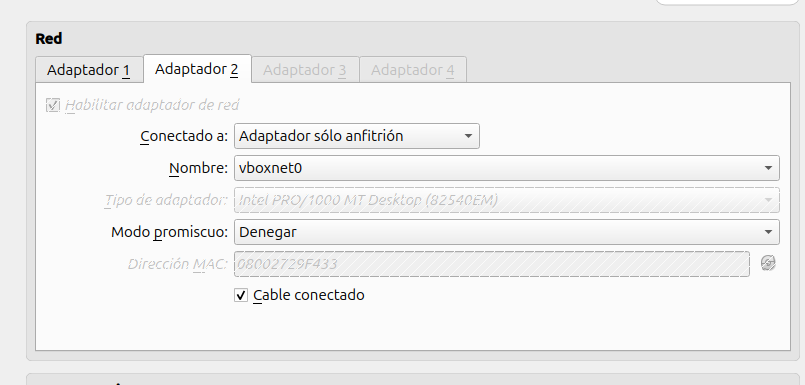
\includegraphics[width=\textwidth]{images/Bloque1/adaptador2.png}
        \caption{Configuración de la red NAT y Host-Only}
    \end{minipage}
    \hfill
    \begin{minipage}[b]{0.45\textwidth}
        \centering
        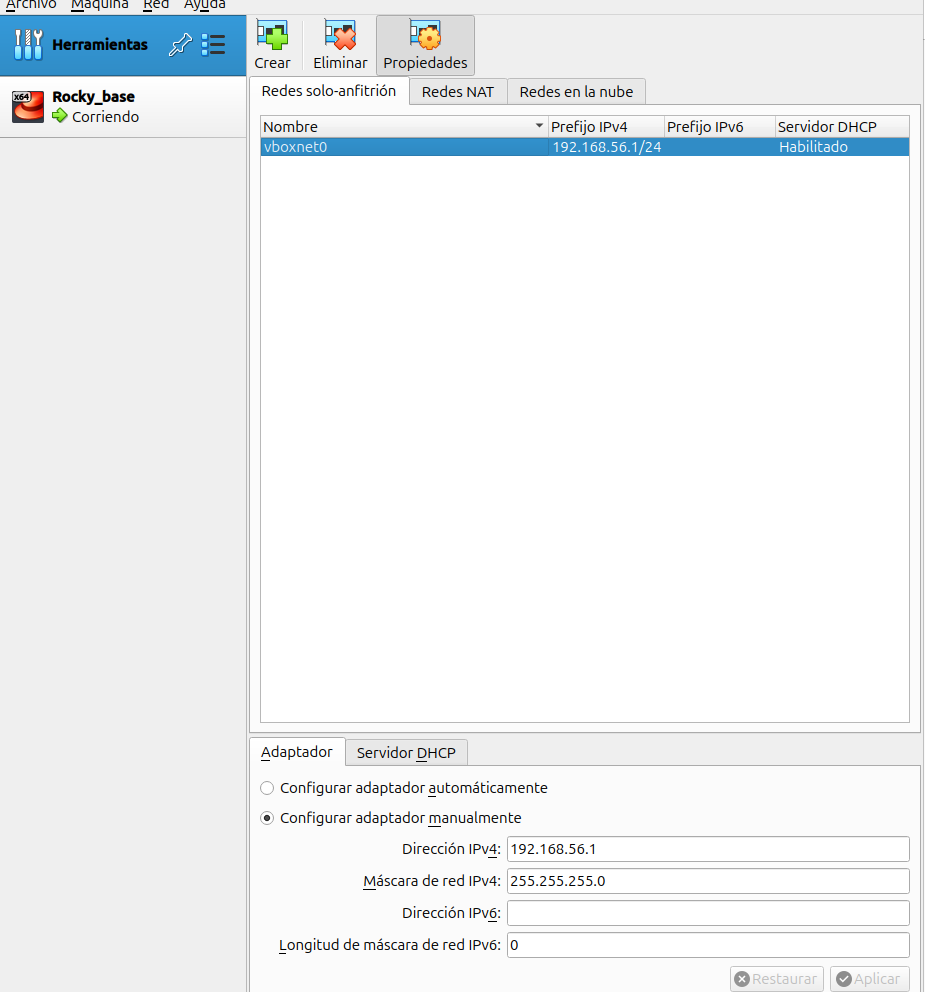
\includegraphics[width=\textwidth]{images/Bloque1/vbox.png}
        \caption{Configuración de VirtualBox para la red de Host-Only}
    \end{minipage}
\end{figure}

Además se nos pide que la Ip de Host Only sea estática, para ello vamos a asegurarnos usando la herramienta \textit{nmtui}, en la que vamos a ver si es estática o no la ip. Como podemos ver en la siguiente imagen esta configurada como ip automática, que viene siendo lo mismo que dinámica por lo que debemos de cambiarlo a manual para poder configurar la ip estática. (Ver Figura 3 y 4). Para ver que efectivamente la ip cambió, podemos verlo en la Figura 5.
\begin{figure}[htbp]
    \centering
    \begin{minipage}[b]{0.45\textwidth}
        \centering
        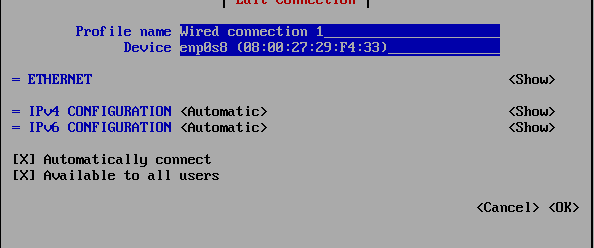
\includegraphics[width=\textwidth]{images/Bloque1/nmtui1.png}
        \caption{Con nmtui vemos que es dinámica}
    \end{minipage}
    \hfill
    \begin{minipage}[b]{0.45\textwidth}
        \centering
        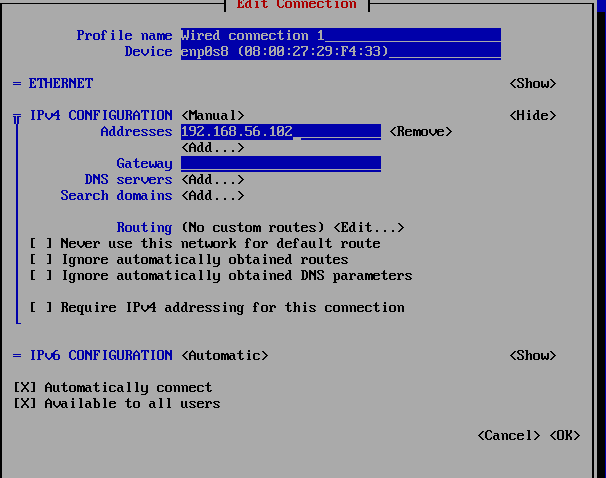
\includegraphics[width=\textwidth]{images/Bloque1/nmtui_2.png}
        \caption{Cambiamos a manual y asignamos una ip estática válida}
    \end{minipage}
\end{figure}



\begin{figure}
    \centering
    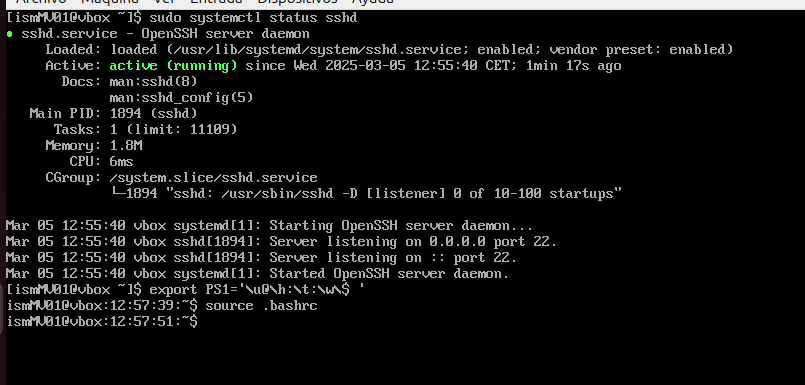
\includegraphics[width=0.8\textwidth]{images/Bloque1/sshd_PS1.png}
    \caption{Sshd y variable PS1}
\end{figure}

\begin{figure}
    \centering
    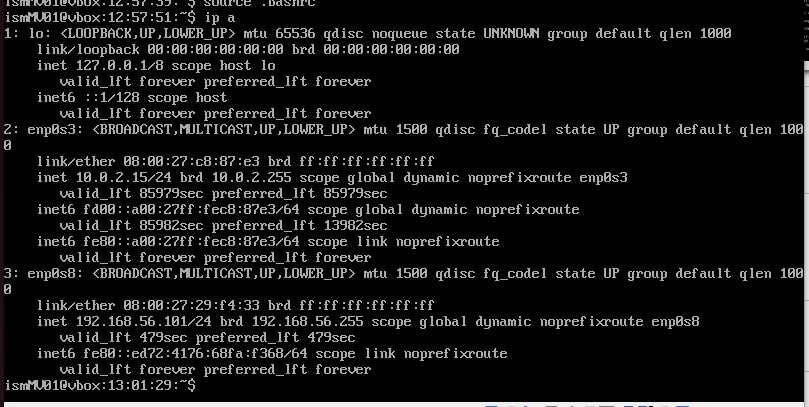
\includegraphics[width=0.8\textwidth]{images/Bloque1/resultado_ipa.png}
    \caption{Resultado de ip a}
\end{figure}

Una vez hayamos cambiado la ip estática, debemos de verificar que efectivamente se ha cambiado y para ello usamos el comando \texttt{ip a} y vemos que efectivamente se ha cambiado la ip a la que hemos asignado. (Ver Figura 7).

\begin{figure}
    \centering
    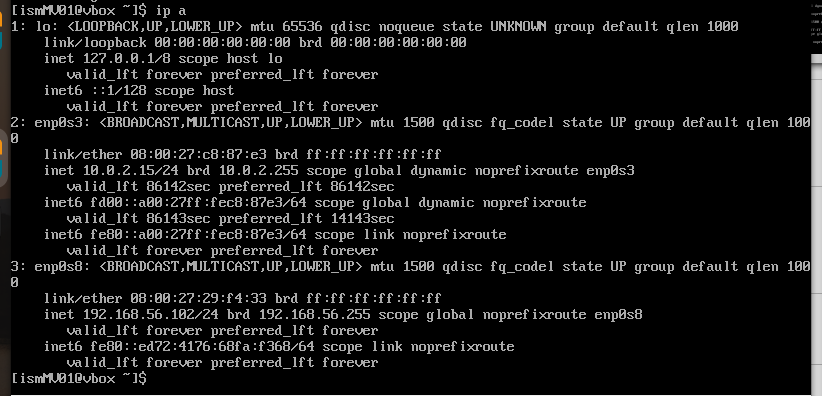
\includegraphics[width=0.8\textwidth]{images/Bloque1/ping2.png}
    \caption{Resultado de ip a para verificar el cambio de ip}
\end{figure}

Llegado a este punto vamos a realizar un ping a la máquina anfitriona y viceversa, para ello usamos el comando \texttt{ping -c <número de pings> ip\_de\_la\_maquina} y vemos que efectivamente hay conexión entre ambas máquinas. (Ver Figura 8, 9 y 10). Además, vemos que gracias al \textit{NAT} podemos hacer ping a cualquier máquina accesible en internet\footnote{Cabe destacar que durante el desarrollo de la actividad, surgían algunas problemas con NetworkManager, polkiy y DBus, pero se solucionaban al reiniciarlos o bien reinstalarlos}. (Ver Figura 11).

\begin{figure}[htbp]
    \centering
    \begin{minipage}[b]{0.45\textwidth}
        \centering
        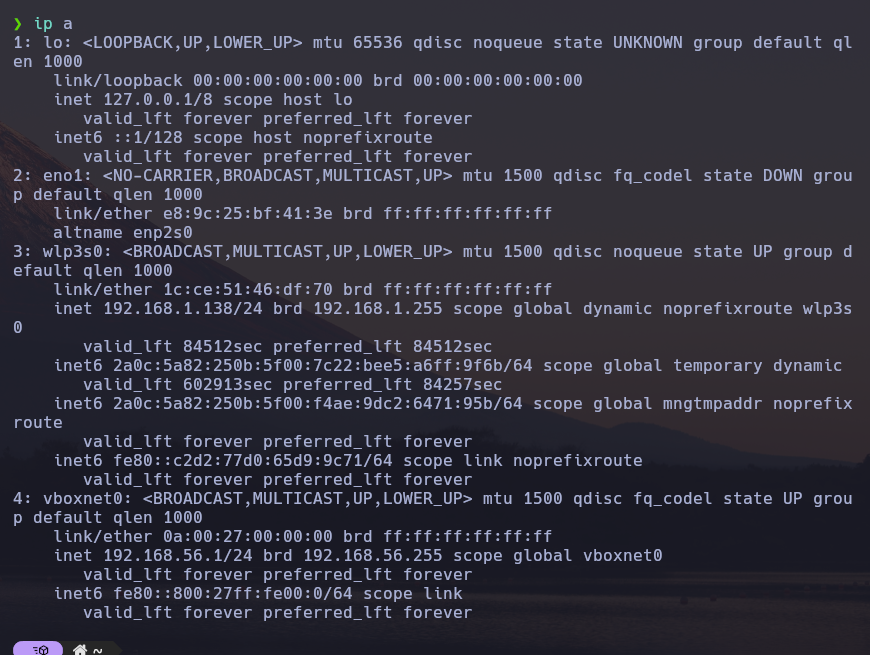
\includegraphics[width=\textwidth]{images/Bloque1/ip_a_host.png}
        \caption{Resultado del comando de \textit{ip a } en la máquina anfitriona para ver la ip}
    \end{minipage}
    \hfill
    \begin{minipage}[b]{0.45\textwidth}
        \centering
        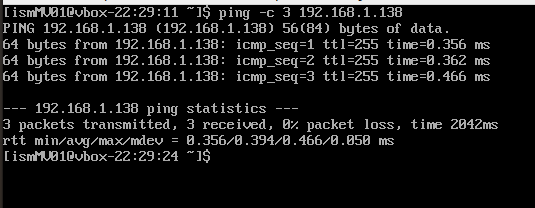
\includegraphics[width=\textwidth]{images/Bloque1/ping_a_anfitriona.png}
        \caption{Ping a la máquina anfitriona}
    \end{minipage}
\end{figure}


\begin{figure}[htbp]
    \centering
    \begin{minipage}[b]{0.45\textwidth}
        \centering
        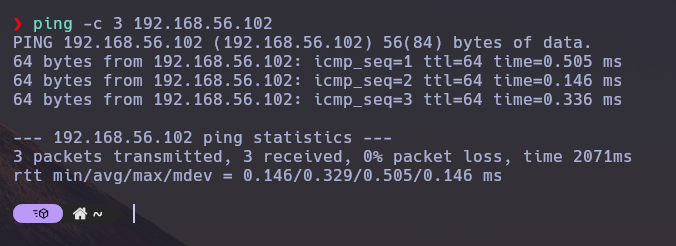
\includegraphics[width=\textwidth]{images/Bloque1/ping_anf_a_mv.png}
        \caption{Ping de la máquina anfitriona a la máquina virtual}
    \end{minipage}
    \hfill
    \begin{minipage}[b]{0.45\textwidth}
        \centering
        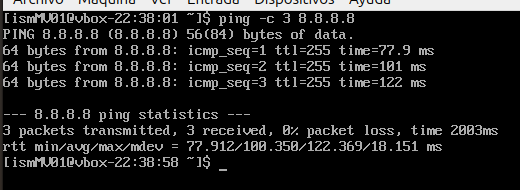
\includegraphics[width=\textwidth]{images/Bloque1/ping_fuera.png}
        \caption{Ping a un servidor público (Google)}
    \end{minipage}
\end{figure}


En cuanto al servicio ssh, debemos de ver el estado del servicio sshd con el comando \texttt{sudo systemctl status sshd} y vemos que esta corriendo. En este punto desde el anfitrión podemos introducirt la línea de comando \texttt{ssh ismMV01@192.168.56.102} y vemos que efectivamente todo funciona correctamente. (Ver Figura 12 y 13).






\begin{figure}[htbp]
    \centering
    \begin{minipage}[b]{0.45\textwidth}
        \centering
        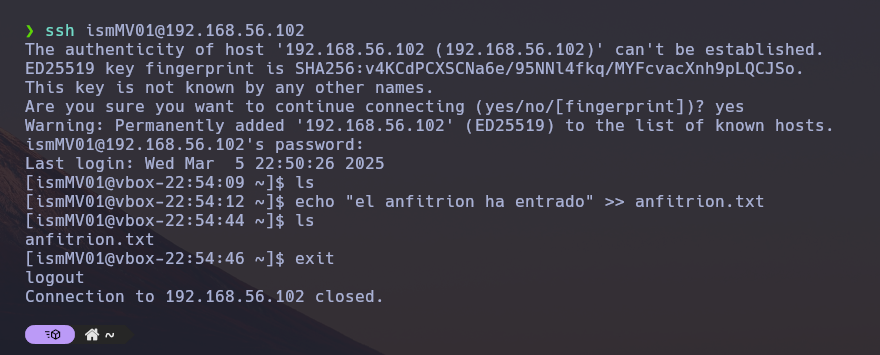
\includegraphics[width=\textwidth]{images/Bloque1/ssh1.png}
        \caption{Ssh en la máquina anfitriona y creación de un archivo en la MV}
    \end{minipage}
    \hfill
    \begin{minipage}[b]{0.45\textwidth}
        \centering
        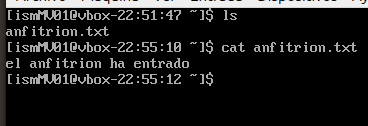
\includegraphics[width=\textwidth]{images/Bloque1/ssh2.png}
        \caption{Ver el contenido del archivo creado en la MV desde el anfitrión}
    \end{minipage}
\end{figure}
\newpage
\section{Servidor con LVM + RAID}

\subsection{Aspectos clave de LVM}

Para gestionar eficazmente el \textit{Logical Volume Manager} (LVM), es fundamental comprender los siguientes componentes y conceptos:

\subsubsection{Componentes de la arquitectura de almacenamiento}

\begin{itemize}
  \item \textbf{Physical Volume (PV)}: Representa los dispositivos de almacenamiento físico, como discos duros o particiones, que se incorporan al sistema LVM.
  \item \textbf{Volume Group (VG)}: Es una agrupación de uno o más PVs que forman un pool de almacenamiento, del cual se pueden asignar espacios para crear volúmenes lógicos.
  \item \textbf{Logical Volume (LV)}: Son volúmenes virtuales creados dentro de un VG. Los LVs se utilizan como si fueran particiones de disco tradicionales, permitiendo la creación de sistemas de archivos o la asignación directa a aplicaciones.
\end{itemize}

\subsubsection{Gestión de almacenamiento con diferentes características físicas}

LVM ofrece flexibilidad para manejar dispositivos de almacenamiento con diversas características físicas:

\begin{itemize}
  \item \textbf{HDD y SSD}: Se pueden combinar en un mismo VG, permitiendo equilibrar rendimiento y capacidad según las necesidades.
  \item \textbf{RAID}: LVM puede trabajar sobre dispositivos RAID, proporcionando una capa adicional de gestión y flexibilidad sobre la configuración RAID existente.
\end{itemize}

\subsubsection{Etiquetado y correspondencia con los archivos de dispositivo}

Cada componente en LVM tiene una nomenclatura específica y se asocia a archivos de dispositivo en el sistema:

\begin{itemize}
  \item \textbf{Physical Volumes}: Corresponden a dispositivos físicos, como \texttt{/dev/sda1}, \texttt{/dev/sdb1}, etc.
  \item \textbf{Volume Groups}: Se nombran según la convención establecida por el administrador, por ejemplo, \texttt{vg\_datos}.
  \item \textbf{Logical Volumes}: Se nombran dentro de su VG correspondiente, como \textit{/dev/vg\_datos/lv\_backup}, donde \textit{lv\_backup} es el nombre del LV.
\end{itemize}

\subsubsection{Comandos de LVM para la gestión de componentes}

LVM proporciona una serie de comandos para administrar sus componentes:

\begin{itemize}
  \item \texttt{pvcreate}: Inicializa un dispositivo físico como PV.
  \item \texttt{vgcreate}: Crea un VG a partir de uno o más PVs.
  \item \texttt{lvcreate}: Crea un LV dentro de un VG.
  \item \texttt{pvs}, \texttt{vgs}, \texttt{lvs}: Muestran información sobre PVs, VGs y LVs respectivamente.
  \item \texttt{pvremove}, \texttt{vgremove}, \texttt{lvremove}: Eliminan PVs, VGs y LVs respectivamente.
\end{itemize}

Estos comandos permiten una gestión eficiente y flexible del almacenamiento en sistemas que utilizan LVM.

\subsection{Niveles de RAID: 0, 1 y 5}

Redundant Array of Independent Disks (RAID) es una tecnología que permite combinar múltiples dispositivos de almacenamiento en una unidad lógica para mejorar el rendimiento, la redundancia o ambos. A continuación, se detallan los niveles de RAID 0, 1 y 5, sus ventajas, desventajas y su administración en sistemas Linux utilizando la herramienta de línea de comandos \texttt{mdadm}.

\subsubsection{RAID 0}

RAID 0, conocido como \textit{striping}, distribuye los datos de manera equitativa entre dos o más discos sin información de paridad ni redundancia.

\begin{itemize}
  \item \textbf{Ventajas}:
    \begin{itemize}
      \item Mayor rendimiento en lectura y escritura debido a la distribución de datos entre los discos.
      \item Uso completo de la capacidad de almacenamiento total, ya que no se reserva espacio para paridad o duplicación.
    \end{itemize}
  \item \textbf{Desventajas}:
    \begin{itemize}
      \item Ausencia de redundancia; la falla de un solo disco resulta en la pérdida total de los datos.
    \end{itemize}
\end{itemize}

\subsubsection{RAID 1}

RAID 1, o \textit{mirroring}, duplica los datos en dos o más discos, creando copias idénticas en cada uno.

\begin{itemize}
  \item \textbf{Ventajas}:
    \begin{itemize}
      \item Alta redundancia; los datos permanecen intactos incluso si uno de los discos falla.
      \item Mejora en la velocidad de lectura, ya que los datos pueden leerse desde cualquiera de los discos.
    \end{itemize}
  \item \textbf{Desventajas}:
    \begin{itemize}
      \item Capacidad de almacenamiento efectiva reducida al 50\% del total, ya que los datos se duplican.
    \end{itemize}
\end{itemize}

\subsubsection{RAID 5}

RAID 5 combina rendimiento y redundancia distribuyendo los datos y la paridad entre tres o más discos.

\begin{itemize}
  \item \textbf{Ventajas}:
    \begin{itemize}
      \item Proporciona tolerancia a fallos; si un disco falla, los datos pueden recuperarse con la información de paridad.
      \item Mejor aprovechamiento del almacenamiento comparado con RAID 1, ya que solo se utiliza una fracción del espacio para la paridad.
    \end{itemize}
  \item \textbf{Desventajas}:
    \begin{itemize}
      \item Rendimiento de escritura inferior al de RAID 0 debido al cálculo de la paridad.
      \item En caso de falla de un disco, la reconstrucción puede ser lenta y afectar el rendimiento.
    \end{itemize}
\end{itemize}

\subsubsection{Administración de RAID en Linux con mdadm}

La herramienta \texttt{mdadm} permite gestionar arreglos RAID en Linux. A continuación, se presentan comandos esenciales:

\begin{itemize}
  \item Crear un RAID 0 con dos discos:
    \begin{lstlisting}[style=mystyle]
    mdadm --create --verbose /dev/md0 --level=0 --raid-devices=2 /dev/sdX /dev/sdY
    \end{lstlisting}
  \item Crear un RAID 1 con dos discos:
    \begin{lstlisting}[style=mystyle]
    mdadm --create --verbose /dev/md0 --level=1 --raid-devices=2 /dev/sdX /dev/sdY
    \end{lstlisting}
  \item Crear un RAID 5 con tres discos:
    \begin{lstlisting}[style=mystyle]
    mdadm --create --verbose /dev/md0 --level=5 --raid-devices=3 /dev/sdX /dev/sdY /dev/sdZ
    \end{lstlisting}
  \item Verificar el estado del RAID:
    \begin{lstlisting}[style=mystyle]
    cat /proc/mdstat
    \end{lstlisting}
  \item Detener un RAID:
    \begin{lstlisting}[style=mystyle]
    mdadm --stop /dev/md0
    \end{lstlisting}
\end{itemize}

\subsection{Aspectos clave para la administración de servidores Linux}

Para implementar eficazmente soluciones en servidores Linux, es esencial comprender y manejar los siguientes aspectos:

\subsubsection{Modos de ejecución y modo de mantenimiento en un servidor Linux}

Los sistemas Linux operan en diferentes niveles de ejecución o \textit{runlevels}, que determinan los servicios y procesos que se ejecutan. Con la adopción de \textit{systemd}, estos niveles se denominan \textit{targets}. El modo de mantenimiento, conocido como \textit{rescue.target} o \textit{emergency.target}, es crucial para tareas de recuperación y administración del sistema. Para cambiar al modo de mantenimiento, se puede utilizar el siguiente comando:

\begin{lstlisting}[style=mystyle]
sudo systemctl isolate rescue.target
\end{lstlisting}

Para volver al modo multiusuario estándar:

\begin{lstlisting}[style=mystyle]
sudo systemctl isolate multi-user.target
\end{lstlisting}

\subsubsection{Estructura estándar del sistema de archivos en Linux}

La estructura de directorios en Linux sigue el estándar de jerarquía de sistemas de archivos (\textit{Filesystem Hierarchy Standard - FHS}). Algunos directorios principales incluyen:

\begin{itemize}
  \item \textbf{/}: Directorio raíz que contiene todos los demás directorios.
  \item \textbf{/bin}: Ejecutables esenciales para todos los usuarios.
  \item \textbf{/etc}: Archivos de configuración del sistema.
  \item \textbf{/home}: Directorios personales de los usuarios.
  \item \textbf{/var}: Datos variables como registros y colas de impresión.
\end{itemize}

\subsubsection{Sistemas de archivos comunes en Linux}

Linux soporta diversos sistemas de archivos. Algunos de los más comunes son:

\begin{itemize}
  \item \textbf{ext4}: Sistema de archivos por defecto en muchas distribuciones, conocido por su estabilidad y rendimiento.
  \item \textbf{XFS}: Adecuado para manejar grandes volúmenes de datos y archivos de gran tamaño.
  \item \textbf{Btrfs}: Ofrece características avanzadas como instantáneas (\textit{snapshots}) y compresión.
\end{itemize}

\subsubsection{Montaje y desmontaje de volúmenes}

El montaje de sistemas de archivos permite acceder a dispositivos de almacenamiento. Para montar un dispositivo:

\begin{lstlisting}[style=mystyle]
sudo mount /dev/sdX1 /mnt/punto_de_montaje
\end{lstlisting}

Para desmontarlo:

\begin{lstlisting}[style=mystyle]
sudo umount /mnt/punto_de_montaje
\end{lstlisting}

Las configuraciones de montaje persistentes se definen en el archivo \texttt{/etc/fstab}.

\subsubsection{Comandos básicos para la gestión de archivos}

La administración de archivos en Linux se realiza mediante comandos de línea. 


% Algunos comandos fundamentales incluyen:

% \begin{itemize}
%   \item \texttt{cp}: Copiar archivos o directorios.
%     \begin{lstlisting}[style=mystyle]
%     cp origen destino
%     \end{lstlisting}
%   \item \texttt{mv}: Mover o renombrar archivos o directorios.
%     \begin{lstlisting}[style=mystyle]
%     mv origen destino
%     \end{lstlisting}
%   \item \texttt{rm}: Eliminar archivos.
%     \begin{lstlisting}[style=mystyle]
%     rm archivo
%     \end{lstlisting}
%   \item \texttt{mkdir}: Crear un nuevo directorio.
%     \begin{lstlisting}[style=mystyle]
%     mkdir nombre_del_directorio
%     \end{lstlisting}
%   \item \texttt{ls}: Listar el contenido de un directorio.
%     \begin{lstlisting}[style=mystyle]
%     ls ruta_del_directorio
%     \end{lstlisting}
%   \item \texttt{cat}: Mostrar el contenido de un archivo.
%     \begin{lstlisting}[style=mystyle]
%     cat archivo
%     \end{lstlisting}
%   \item \texttt{nano} o \texttt{vim}: Editores de texto para modificar archivos desde la terminal.
%     \begin{lstlisting}[style=mystyle]
%     nano archivo
%     \end{lstlisting}
% \end{itemize}

% Estos comandos son esenciales para la gestión diaria de archivos y directorios en un entorno Linux.
Estos se deben de haber estudiado en asignaturas anteriores como Sistemas Operativos.

\subsection{Ejercicio Opcional}

Partiendo de un servidor básico configurado de acuerdo al apartado 2, el alumno/a deberá
afrontar el caso práctico descrito a continuación:

Se desea instalar un servicio de gestión documental en el servidor. Se espera que este servicio
precise de una cantidad espacio de almacenamiento creciente con el tiempo, pudiendo llegar a
ser considerable.

Por otro lado, el contenido será crítico, por lo que se desea proporcionar
algún mecanismo de respaldo ante fallos en el dispositivo de almacenamiento.

El alumno/a debe diseñar los cambios en el sistema de almacenamiento e implementarlo
empleando prácticas adecuadas de administración que garanticen la conservación de la
información en el sistema y procuren la máxima disponibilidad del servicio.

\subsubsection{Solución}

Para la resolución de este ejercicio vamos a seguir lo realizado en clase. (Ver apuntes de clase correspondientes a la sección de LVM+RAID).

En primer lugar creamos los discos, para ello entramos en la configuración de la máquina virtual y añadimos dos discos duros de 1GB cada uno. Una vez añadidos los discos duros, iniciamos la máquina virtual y ejecutamos el comando \texttt{lsblk} para ver los discos duros que tenemos disponibles. (Ver Figura 14).

\begin{figure}[htbp]
  \centering
  \begin{minipage}[b]{0.45\textwidth}
      \centering
      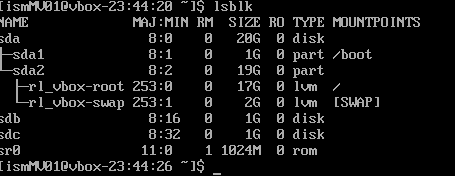
\includegraphics[width=\textwidth]{images/Bloque1/lsblk.png}
      \caption{Resultado del comando lsblk}
  \end{minipage}
  \hfill
  \begin{minipage}[b]{0.45\textwidth}
      \centering
      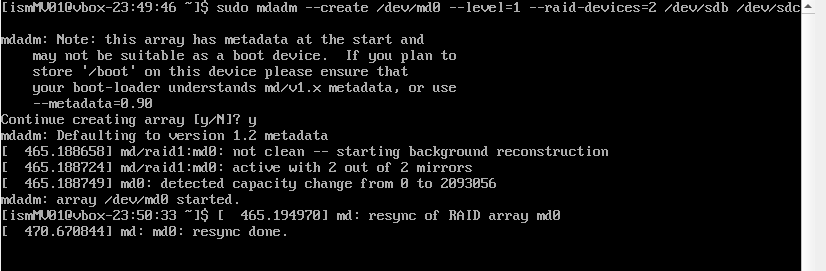
\includegraphics[width=\textwidth]{images/Bloque1/mdadm.png}
      \caption{Comando mdadm}
  \end{minipage}
\end{figure}

A continuación, instalamos \textit{mdadm} con el comando \texttt{sudo dnf install -y mdadm} y creamos un RAID 1 con los dos discos duros que hemos añadido. Para ello ejecutamos el comando \texttt{sudo mdadm --create --verbose /dev/md0 --level=1 --raid-devices=2 /dev/sdb /dev/sdc} y vemos que se ha creado correctamente. (Ver Figura 15).

Acto seguido debemos de crear un PV, VG y LV. Para ello ejecutamos los siguientes comandos (Ver Figura 16):
\begin{itemize}
  \item \texttt{sudo pvcreate /dev/md0}
  \item \texttt{sudo vgcreate vg\_datos /dev/md0}
  \item \texttt{sudo lvcreate -L 900M -n lv\_datos vg\_datos}
\end{itemize}

\begin{figure}[htbp]
  \centering
  \begin{minipage}[b]{0.45\textwidth}
      \centering
      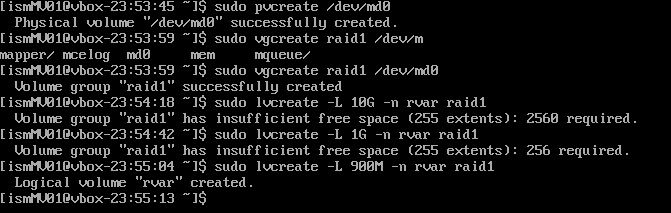
\includegraphics[width=\textwidth]{images/Bloque1/create.png}
      \caption{Resultado de crear los volúmenes}
  \end{minipage}
  \hfill
  \begin{minipage}[b]{0.45\textwidth}
      \centering
      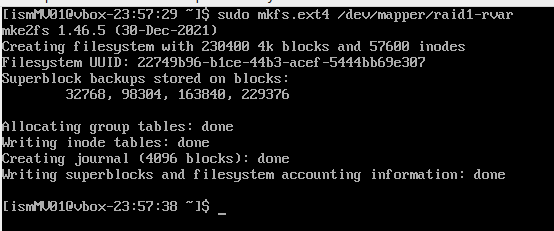
\includegraphics[width=\textwidth]{images/Bloque1/mkfs.png}
      \caption{Comando mkfs}
  \end{minipage}
\end{figure}

Ahora debemos de formatear el volumen lógico en formato ext4. (Ver Figura 17).

A continuación, montamos (Ver Figura 18) y trasladamos la carpeta \textit{var} al nuevo volumen lógico. Para ello ejecutamos los comando que figuran en los apuntes de clase.

\begin{figure}[htbp]
  \centering
  \begin{minipage}[b]{0.45\textwidth}
      \centering
      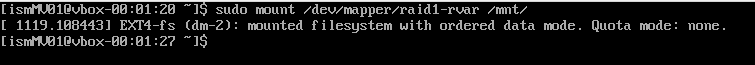
\includegraphics[width=\textwidth]{images/Bloque1/mount.png}
      \caption{Resultado del comando mount}
  \end{minipage}
  \hfill
  \begin{minipage}[b]{0.45\textwidth}
      \centering
      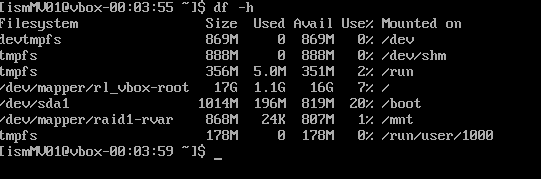
\includegraphics[width=\textwidth]{images/Bloque1/df.png}
      \caption{Comando df -h}
  \end{minipage}
\end{figure}

  Ejecutamos el comando \texttt{df -h} para ver que efectivamente se ha montado correctamente el volumen lógico. (Ver Figura 19).

  Ejecutamos el isolate del systemctl para entrar en modo de mantenimiento y poder trasladar la carpeta \textit{var} al nuevo volumen lógico. (Ver Figura 20).

  \begin{figure}[htbp]
    \centering
    \begin{minipage}[b]{0.45\textwidth}
        \centering
        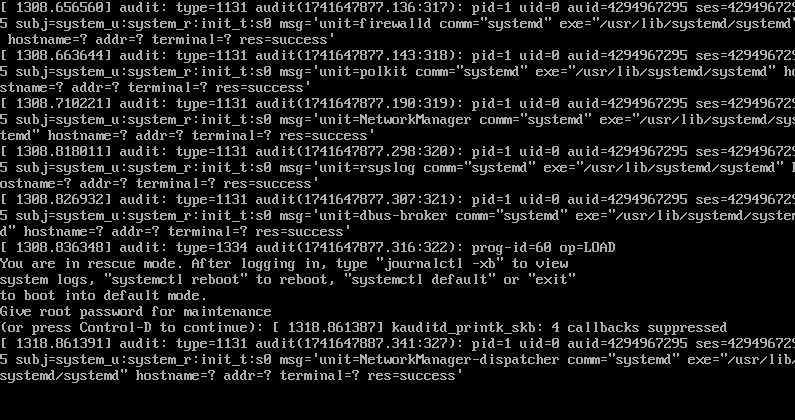
\includegraphics[width=\textwidth]{images/Bloque1/isolate.png}
        \caption{Resultado del comando systemctl isolate}
    \end{minipage}
    \hfill
    \begin{minipage}[b]{0.45\textwidth}
        \centering
        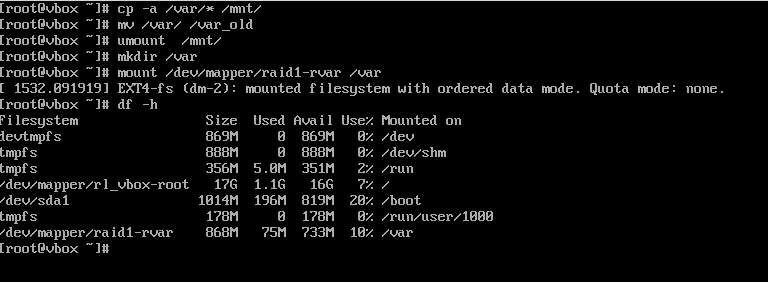
\includegraphics[width=\textwidth]{images/Bloque1/var.png}
        \caption{Serie de operaciones para trasladar la carpeta var}
    \end{minipage}
  \end{figure}

Ahora debemos de trabajar con la serie de comandos que se especifican para poder mover la carpeta y que se haga de forma correcta. (Ver Figura 21).

Una vez trasladad la carpeta, debemos de hacer permanentes los cambios, para ello debemos de editar el fichero \texttt{/etc/fstab} y añadir la siguiente línea (Ver Figura 22):

\begin{lstlisting}[style=mystyle]
  /dev/mapper/raid1-rvar /var ext4 defaults 0 0
\end{lstlisting}

Recargamos la configuraciones con el deamon de systemd y vemos que aparece la parte que estabamos montando (Ver Figura 23).

\begin{figure}[htbp]
  \centering
  \begin{minipage}[b]{0.45\textwidth}
      \centering
      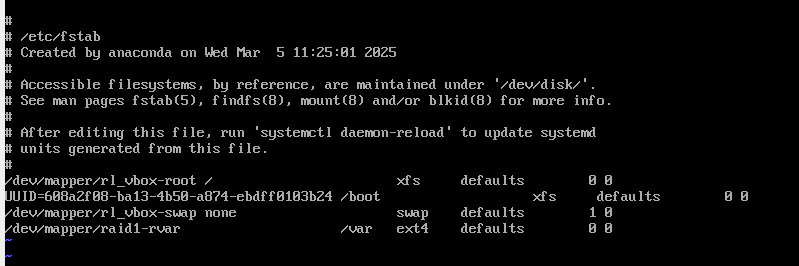
\includegraphics[width=\textwidth]{images/Bloque1/fstab.png}
      \caption{Resultado de editar /etc/fstab como se indica}
  \end{minipage}
  \hfill
  \begin{minipage}[b]{0.45\textwidth}
      \centering
      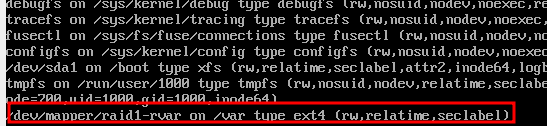
\includegraphics[width=\textwidth]{images/Bloque1/daemon.png}
      \caption{Resultado del comando systemctl daemon-reload y mount}
  \end{minipage}
\end{figure}

Y como podemos comprobar en la Figura 24, hemos conseguido trasladar la carpeta \textit{var} al nuevo volumen lógico y todo funciona correctamente.

\begin{figure}[H]
  \centering
  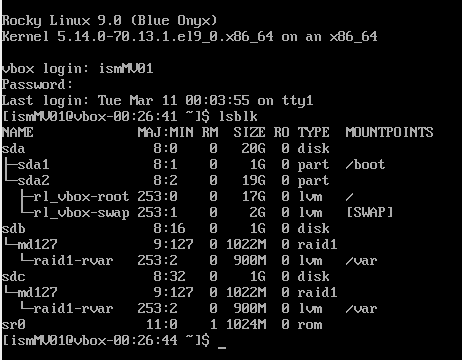
\includegraphics[width=0.6\textwidth]{images/Bloque1/resultadofinal_raid.png}
  \caption{Resultado final}
\end{figure}

\newpage
\section{Acceso seguro al servidor: Firewall + SSHD}

\subsection{Iptables}

\texttt{iptables} es una herramienta de línea de comandos utilizada para configurar el cortafuegos en el núcleo de Linux, implementado dentro del proyecto Netfilter. Aunque \texttt{iptables} es un marco heredado, \texttt{nftables} se presenta como su reemplazo moderno, ofreciendo una capa de compatibilidad. 

\subsubsection{Instalación}

El núcleo estándar de Arch Linux viene compilado con soporte para \texttt{iptables}. Para instalar las utilidades de usuario, se debe instalar el paquete \texttt{iptables}, que es una dependencia indirecta del metapaquete \texttt{base}, por lo que debería estar instalado por defecto en el sistema. 

\subsubsection{Conceptos Básicos}

\begin{itemize}
    \item \textbf{Tablas}: Colecciones de reglas con propósitos específicos.
    \item \textbf{Cadenas}: Listas de reglas dentro de una tabla que se recorren en orden.
    \item \textbf{Reglas}: Definiciones que consisten en un criterio de coincidencia y una acción a ejecutar si se cumple dicho criterio.
\end{itemize}

\subsubsection{Configuración y Uso}

\texttt{iptables} se puede configurar directamente desde la línea de comandos o mediante diversas interfaces frontales, tanto de consola como gráficas. Para mostrar las reglas actuales, se utiliza:

\begin{verbatim}
iptables -L
\end{verbatim}

Para restablecer las reglas:

\begin{verbatim}
iptables -F
\end{verbatim}

\subsubsection{Registro de Actividad}

\texttt{iptables} permite registrar paquetes para monitorear actividad o depurar reglas. Es posible limitar la tasa de registro para evitar la saturación de los registros del sistema. 
\subsubsection{Alternativas y Herramientas Relacionadas}

\begin{itemize}
    \item \textbf{\texttt{nftables}}: Proyecto que busca reemplazar a \texttt{iptables}, proporcionando un nuevo marco de filtrado de paquetes y una utilidad de espacio de usuario llamada \texttt{nft}. 
    \item \textbf{\texttt{ipset}}: Aplicación complementaria que permite crear conjuntos de direcciones IP para ser utilizados en reglas de \texttt{iptables}, facilitando el bloqueo o la aceptación de múltiples direcciones de manera eficiente. 
    \item \textbf{\texttt{ufw} (Uncomplicated Firewall)}: Programa para gestionar el cortafuegos de manera sencilla, proporcionando una interfaz de línea de comandos fácil de usar. 
\end{itemize}

\subsubsection{Recursos Adicionales}

Para configuraciones más avanzadas, como la creación de un cortafuegos con estado o compartir la conexión a Internet, se pueden consultar las siguientes guías:

\begin{itemize}
    \item \textbf{Cortafuegos con Estado Sencillo}: Explica cómo configurar un cortafuegos con estado utilizando \texttt{iptables}, detallando las reglas necesarias y su propósito. 
    \item \textbf{Compartir Conexión a Internet}: Describe cómo compartir la conexión a Internet desde una máquina a otras, incluyendo los requisitos y pasos necesarios.
\end{itemize}


\subsection{firewalld y firewall-cmd en Rocky Linux}

\texttt{firewalld} es un servicio de cortafuegos dinámico que permite gestionar reglas de firewall sin necesidad de reiniciar el servicio. Su herramienta de línea de comandos, \texttt{firewall-cmd}, proporciona una interfaz para la administración del firewall en sistemas como Rocky Linux.

\subsubsection{Gestión del Firewall con firewall-cmd}

\texttt{firewall-cmd} permite configurar reglas de firewall de manera flexible y en tiempo real. Algunas de las operaciones más comunes incluyen:

\begin{itemize}
    \item \textbf{Verificar el estado del firewall}:
    \begin{verbatim}
    firewall-cmd --state
    \end{verbatim}

    \item \textbf{Listar las reglas activas}:
    \begin{verbatim}
    firewall-cmd --list-all
    \end{verbatim}

    \item \textbf{Abrir un puerto específico} (ejemplo: puerto 80 TCP):
    \begin{verbatim}
    firewall-cmd --add-port=80/tcp --permanent
    \end{verbatim}
    
    \item \textbf{Cerrar un puerto específico}:
    \begin{verbatim}
    firewall-cmd --remove-port=80/tcp --permanent
    \end{verbatim}

    \item \textbf{Recargar la configuración del firewall} para aplicar cambios:
    \begin{verbatim}
    firewall-cmd --reload
    \end{verbatim}
\end{itemize}

\subsubsection{Administración del Servicio firewalld con systemctl}

\texttt{systemctl} es una herramienta utilizada para gestionar servicios en sistemas basados en \texttt{systemd}, como Rocky Linux. Se puede utilizar para controlar el servicio \texttt{firewalld} de la siguiente manera:

\begin{itemize}
    \item \textbf{Verificar si el servicio está activo}:
    \begin{verbatim}
    systemctl status firewalld
    \end{verbatim}

    \item \textbf{Iniciar el servicio} si está detenido:
    \begin{verbatim}
    systemctl start firewalld
    \end{verbatim}

    \item \textbf{Detener el servicio} si se necesita desactivarlo temporalmente:
    \begin{verbatim}
    systemctl stop firewalld
    \end{verbatim}

    \item \textbf{Habilitar el servicio para que se inicie automáticamente} al arrancar el sistema:
    \begin{verbatim}
    systemctl enable firewalld
    \end{verbatim}

    \item \textbf{Deshabilitar el servicio para evitar su inicio automático}:
    \begin{verbatim}
    systemctl disable firewalld
    \end{verbatim}
\end{itemize}

\subsubsection{Verificación de Configuración con nmap}

\texttt{nmap} es una herramienta de escaneo de redes que permite verificar los puertos abiertos y configuraciones de firewall. Se puede usar para comprobar la efectividad de las reglas de firewall aplicadas. Algunos ejemplos de uso incluyen:

\begin{itemize}
    \item \textbf{Escanear los puertos abiertos de una dirección IP específica}:
    \begin{verbatim}
    nmap <direccion_ip>
    \end{verbatim}

    \item \textbf{Escanear puertos específicos} (ejemplo: puertos 22 y 80):
    \begin{verbatim}
    nmap -p 22,80 <direccion_ip>
    \end{verbatim}

    \item \textbf{Detectar el sistema operativo del host analizado}:
    \begin{verbatim}
    nmap -O <direccion_ip>
    \end{verbatim}
\end{itemize}

Estas herramientas permiten una administración avanzada del firewall en Rocky Linux, garantizando la seguridad de la red y el control del tráfico de red en el sistema.

\subsection{Ejercicio Opcional}

Como caso práctico, partiendo de una MV con la configuración base descrita en el apartado 2, el
alumno/a deberá ser capaz de instalar un servidor de HTTP, Apache o Nginx,
y habilitar/deshabilitar su acceso por Firewall.

Para ello, instalará el servidor web de su elección y modificará la home page para mostrar un
mensaje:'Bienvenidos a la web de <Nombre y Apellidos del alumno/a> en Prácticas ISE'.

El servicio web debe estar accesible en la servidor (MV) en el puerto por defecto (80) usando un
navegador web convencional corriendo en el anfitrión (Host).

Un escaneo de puertos sobre el servidor solo debe mostrar como accesibles los puerto web y ssh.

\subsection*{Solución}

Para la resolución de este ejercicio vamos a seguir los siguientes pasos:

\begin{enumerate}
\item Instalamos el servidor web Apache con el comando \micode{sudo dnf install -y httpd}. También tenemos la opción de instalar Nginx con el comando \micode{sudo dnf install nginx- y}. \textit{Tenemos libre elección de servidor web, en mi caso será Apache}.
\item Debemos de activar este servicio con el comando:
  \begin{itemize}
    \item Apache: \micode{sudo systemctl enable httpd --now}
    \item Nginx: \micode{sudo systemctl enable nginx --now}
    \item Debemos de verificar que el servicio esta activo con los comandos:
    \begin{itemize}
      \item \micode{sudo systemctl status httpd # Para Apache}
      \item \micode{sudo systemctl status nginx # Para Nginx}
    \end{itemize}
  \end{itemize}
  \item Modificación de la página principal.\\
  Debemos de personalizar la página de inicio de nuestra web para que muestre el mensaje que se nos pide en el enunciado.
  \begin{itemize}
    \item Apache: \micode{echo "Bienvenidos a la web de <Nombre y Apellidos> en Prácticas ISE" | sudo tee /var/www/html/index.html}
    \item Nginx: \micode{echo "Bienvenidos a la web de <Nombre y Apellidos> en Prácticas ISE" | sudo tee /usr/share/nginx/html/index.html}
  \end{itemize}
  \item Configuración del Firewall.\\
  Para permitir el acceso a la web, es necesario abrir el puerto 80 en el firewall. Para ello, ejecutamos los siguientes comandos:
  \begin{itemize}
    \item \micode{sudo firewall-cmd --add-service=http --permanent}
    \item \micode{sudo firewall-cmd --reload}
    \item Para verificar que el puerto esta abierto: \micode{sudo firewall-cmd --list-all}
  \end{itemize}
  \item Acceder desde el Navegador.\\
  Si todo está configurado correctamente, se visualizará el mensaje personalizado\footnote{Para saber a que ip acceder, podemos usar el comando \textit{ip a} y coger la correspondiente a \textit{enp0s8.}}(Ver Figura \ref{web}).
  \begin{figure}[H]
    \centering
      
\includegraphics[width=0.7\textwidth]{images/Bloque1/web.png}
      \caption{Acceso a la web desde el navegador}
      \label{web}
  \end{figure}
  \item Restricción de puertos con Firewall.\\
  Para asegurar que solo los puertos web (80) y SSH (22) estén accesibles, se deben eliminar
otras reglas de firewall:
\begin{itemize}
  \item \micode{sudo firewall-cmd --list-services --permanent}\footnote{Con este comando podemos ver los servicios que están activos en el firewall, desactivamos todos, a excepción de http y ssh.}
  \item \micode{sudo firewall-cmd --remove-service=<nombre> --permanent}
  \item \micode{sudo firewall-cmd --reload}
  \item Extra.\\
  Como extra podemos ver los puertos que están abiertos con el comando \micode{sudo firewall-cmd --list-ports --permanent} y cerramos el puerto con \micode{sudo firewall-cmd --remove-port=xxxx/tcp --permanent}, donde xxxx es el puerto que queremos cerrar. Otra forma de solo tener dos puertos abiertos es con los comandos:
  \begin{itemize}
    \item \micode{sudo firewall-cmd --add-service=http --permanent}
    \item \micode{sudosudo firewall-cmd --add-service=ssh --permanent}
    \item Y de nuevo recargamos y listamos todos los puertos.
  \end{itemize}
\end{itemize}
\end{enumerate}

\newpage
\section{SSH}

\subsection{Administración remota con SSH y criptografía asimétrica}

La administración remota es una tarea fundamental en la gestión de servidores. Una de las herramientas más utilizadas para este propósito es \texttt{SSH} (Secure Shell), que permite acceder y administrar un sistema de manera segura a través de una red. Es importante destacar que \texttt{SSH} puede referirse tanto a un cliente como a un servicio.

\subsubsection{Instalación y configuración de SSH}
Para instalar y habilitar el servicio SSH en un sistema basado en Rocky Linux, se utilizan los siguientes comandos:

\begin{lstlisting}[style=mystyle]
sudo dnf install -y openssh-server
sudo systemctl enable --now sshd
\end{lstlisting}

El servicio \texttt{sshd} es el demonio que permite las conexiones SSH entrantes. Su configuración se encuentra en el archivo:

\begin{lstlisting}[style=mystyle]
/etc/ssh/sshd_config
\end{lstlisting}

Al editar este archivo, es posible modificar diversas opciones de seguridad, como:

\begin{itemize}
    \item \textbf{Deshabilitar el acceso como root por contraseña:} Para mejorar la seguridad, se recomienda restringir el acceso directo de root:
    \begin{lstlisting}[style=mystyle]
    PermitRootLogin no
    \end{lstlisting}
    
    \item \textbf{Cambio de puerto predeterminado:} SSH por defecto usa el puerto 22, pero puede cambiarse para reducir ataques automatizados:
    \begin{lstlisting}[style=mystyle]
    Port 2222
    \end{lstlisting}
\end{itemize}

Después de modificar la configuración, es necesario reiniciar el servicio:

\begin{lstlisting}[style=mystyle]
sudo systemctl restart sshd
\end{lstlisting}

\subsubsection{Configuración del firewall para SSH}
Si se cambia el puerto de \texttt{SSH}, es necesario actualizar la configuración del firewall:

\begin{lstlisting}[style=mystyle]
sudo firewall-cmd --add-port=2222/tcp --permanent
sudo firewall-cmd --reload
\end{lstlisting}

\subsubsection{Criptografía simétrica y asimétrica en SSH}
\textbf{Criptografía simétrica} es un método en el que la misma clave se usa tanto para cifrar como para descifrar los datos. Es rápida pero menos segura para la comunicación remota, ya que ambas partes deben compartir la clave de forma segura.

\textbf{Criptografía asimétrica}, utilizada en SSH, emplea un par de claves: una clave pública y una clave privada. El cliente genera un par de claves y comparte la clave pública con el servidor, lo que permite autenticarse sin necesidad de enviar una contraseña.

Para generar un par de claves en SSH, se usa:

\begin{lstlisting}[style=mystyle]
ssh-keygen -t rsa -b 4096
\end{lstlisting}

Y para copiar la clave pública al servidor:

\begin{lstlisting}[style=mystyle]
ssh-copy-id usuario@servidor
\end{lstlisting}

Esto permite autenticarse sin necesidad de contraseña, mejorando la seguridad y facilitando la automatización de tareas en servidores remotos.

\subsection{Ejercicio Opcional}

Partiendo de un servidor base configurado siguiendo las indicaciones del apartado 2, el
alumno/a modificará servicio SSHD para que, en lugar del puerto por defecto (22), se ejecute en
un puerto alternativo de un valor mayor a 1024. Se recomienda que consulte la lista de puertos
reconocidos por el sistema en /etc/ports para evitar emplear un puerto que ya tenga una
aplicación predefinida.

Se concederá acceso remoto por llave pública a un usuario de su elección.
El ejercicio se validará ejecutando un comando de forma remota sobre el servidor SSH con la
nueva configuración. El comando presentará el contenido completo (incluido ficheros y
directorios ocultos) con del directorio home del usuario remoto empleado en la conexión. Para
ello, desde el ordenador anfitrión (o una MV distinta a la que se va a acceder) se empleará ssh
sin terminal remoto y sin contraseña, pasando como único como parámetro el comando a
ejecutar.

\subsection*{Solución}

\subsection*{Modificación del servicio SSHD y acceso remoto por llave pública}

En este ejercicio, se modificará la configuración del servicio SSH para que utilice un puerto alternativo y se habilitará el acceso remoto mediante autenticación con clave pública.

\subsubsection*{Paso 1: Verificar puertos disponibles}

Antes de modificar la configuración de SSH, es recomendable consultar la lista de puertos reconocidos por el sistema para evitar conflictos con otros servicios. Para ello, se puede inspeccionar el archivo:

\begin{lstlisting}[style=mystyle]
cat /etc/services | less
\end{lstlisting}

Se debe elegir un puerto mayor a 1024 que no esté en uso.

\subsubsection*{Paso 2: Modificar la configuración de SSH}

Editar el archivo de configuración de SSH con un editor de texto como `vim` o `nano`:

\begin{lstlisting}[style=mystyle]
sudo nano /etc/ssh/sshd_config
\end{lstlisting}

Buscar la línea que especifica el puerto (`\#Port 22`), descomentarla y cambiarla por el número de puerto elegido, por ejemplo:

\begin{lstlisting}[style=mystyle]
Port 2222
\end{lstlisting}

Guardar los cambios y salir del editor.

\subsubsection{Solución al error al cambiar el puerto de SSH}

Si al cambiar el puerto en la configuración de SSH y reiniciar el servicio se obtiene un error, se deben seguir los siguientes pasos para solucionar el problema:

\begin{enumerate}
    \item \textbf{Verificar errores en la configuración de SSH}  
    Ejecutar el siguiente comando para comprobar si hay errores en el archivo de configuración:

    \begin{lstlisting}[style=mystyle]
    sudo sshd -t
    \end{lstlisting}

    Si se detectan errores de sintaxis o configuración en el archivo \textit{/etc/ssh/sshd\_config}, se deben corregir antes de continuar.

    \item \textbf{Confirmar que el puerto está permitido en SELinux (si aplica)}  
    Si el sistema usa SELinux, es necesario permitir el nuevo puerto:

    \begin{lstlisting}[style=mystyle]
    sudo semanage port -a -t ssh_port_t -p tcp 2222
    \end{lstlisting}

    Si el comando \texttt{semanage} no está disponible, se puede instalar con:

    \begin{lstlisting}[style=mystyle]
    sudo dnf install policycoreutils-python-utils
    \end{lstlisting}

    Luego, verificar que el puerto se agregó correctamente con:

    \begin{lstlisting}[style=mystyle]
    sudo semanage port -l | grep ssh
    \end{lstlisting}

    \item \textbf{Permitir el nuevo puerto en \texttt{firewalld}}  
    Si el sistema usa \texttt{firewalld}, se debe agregar el puerto y recargar la configuración:

    \begin{lstlisting}[style=mystyle]
    sudo firewall-cmd --permanent --add-port=2222/tcp
    sudo firewall-cmd --reload
    \end{lstlisting}

    \item \textbf{Reiniciar el servicio SSH y comprobar su estado}  
    Una vez realizados los cambios, reiniciar el servicio SSH:

    \begin{lstlisting}[style=mystyle]
    sudo systemctl restart sshd
    \end{lstlisting}

    Si el servicio sigue fallando, revisar los logs para obtener más detalles sobre el error:

    \begin{lstlisting}[style=mystyle]
    sudo journalctl -xeu sshd
    \end{lstlisting}
\end{enumerate}

Siguiendo estos pasos, se podrá cambiar el puerto de SSH sin problemas y reiniciar el servicio correctamente.


\subsubsection*{Paso 3: Ajustar firewalld para permitir conexiones en el nuevo puerto}

Si `firewalld` está en uso, es necesario agregar el nuevo puerto al firewall y eliminar el acceso al puerto 22 si no se desea que permanezca abierto:

\begin{lstlisting}[style=mystyle]
sudo firewall-cmd --permanent --add-port=2222/tcp
sudo firewall-cmd --permanent --remove-service=ssh
sudo firewall-cmd --reload
\end{lstlisting}

\subsubsection*{Paso 4: Reiniciar el servicio SSH}

Aplicar los cambios reiniciando el servicio SSH:

\begin{lstlisting}[style=mystyle]
sudo systemctl restart sshd
\end{lstlisting}

\subsubsection*{Paso 5: Configurar autenticación por clave pública}

Desde el cliente, generar un par de claves SSH si no se tienen:

\begin{lstlisting}[style=mystyle]
ssh-keygen -t rsa -b 4096
\end{lstlisting}

Copiar la clave pública al servidor(Ver Figura \ref{copiaLlave}):

\begin{lstlisting}[style=mystyle]
ssh-copy-id -p 2222 usuario@IP_del_Servidor
\end{lstlisting}

\begin{figure}[H]
  \centering
  \begin{minipage}[b]{0.45\textwidth}
    \centering
    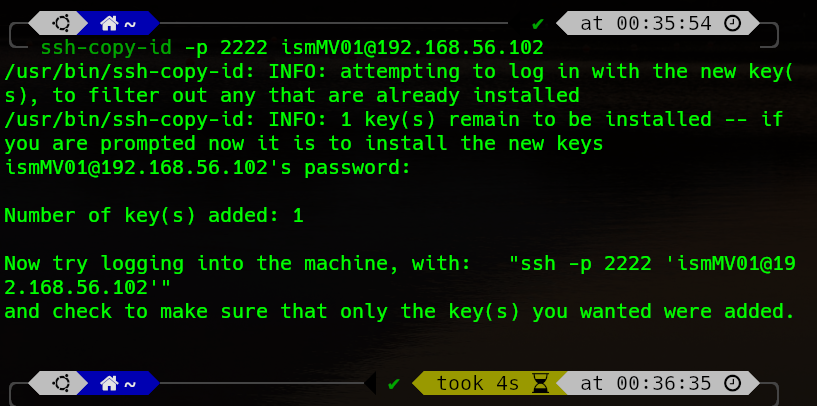
\includegraphics[width=\textwidth]{images/copiaLlave.png}
    \caption{SSH en mi máquina}
    \label{copiaLlave}
  \end{minipage}
  \hfill
  \begin{minipage}[b]{0.45\textwidth}
    \centering
    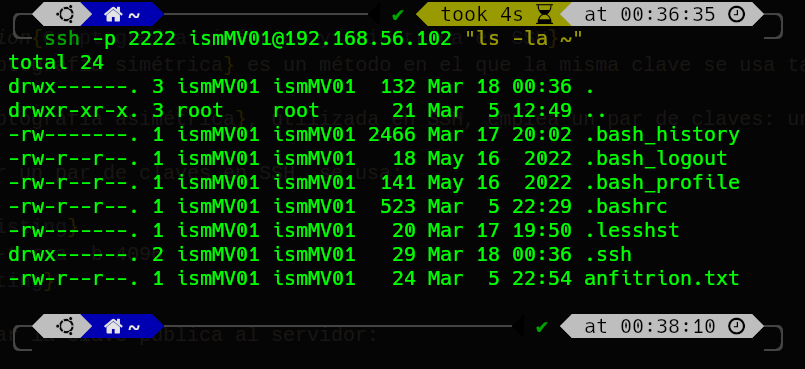
\includegraphics[width=\textwidth]{images/finalSSH.png}
    \caption{SSH final}
    \label{finalSSH}
  \end{minipage}
\end{figure}

\subsubsection*{Paso 6: Validar la conexión sin contraseña}

Para comprobar que el acceso es correcto, se ejecutará un comando remoto en la máquina virtual desde otro equipo o una máquina anfitriona. Se listará el contenido completo del directorio home del usuario remoto, incluidos los archivos ocultos (Ver Figura \ref{finalSSH}):

\begin{lstlisting}[style=mystyle]
ssh -p 2222 usuario@IP_del_Servidor "ls -la ~"
\end{lstlisting}

Si todo está configurado correctamente, el comando mostrará los archivos del directorio home sin requerir contraseña.

\newpage
\section{Automatización de la configuración con Ansible}

\subsection{Introducción a Ansible}

Ansible es una herramienta de automatización que permite gestionar configuraciones y despliegues en múltiples sistemas de manera sencilla y eficiente. Su funcionamiento se basa en la ejecución de comandos remotos a través de SSH y utiliza Python como lenguaje de scripting, lo que facilita su integración en la mayoría de las distribuciones Linux.

\subsubsection{Comandos Ad-Hoc en Ansible}

Los comandos ad-hoc en Ansible permiten ejecutar tareas únicas y rápidas en uno o varios nodos gestionados sin necesidad de crear un playbook. Se utilizan a través de la herramienta de línea de comandos \texttt{ansible} y son ideales para operaciones puntuales, como reiniciar servicios, copiar archivos o instalar paquetes. Aunque son fáciles de usar, no son reutilizables ni idempotentes, por lo que para tareas repetitivas o complejas se recomienda el uso de playbooks. \cite{turn0search0}

\subsubsection{Módulos de Ansible}

Ansible cuenta con una amplia variedad de módulos que encapsulan tareas específicas, como gestionar usuarios, instalar paquetes o manejar servicios. Estos módulos permiten abstraer la complejidad de las operaciones subyacentes y proporcionan una interfaz consistente para interactuar con diferentes sistemas y servicios. La documentación oficial de Ansible ofrece un índice completo de todos los módulos disponibles, organizados por categorías, facilitando la búsqueda y selección del módulo adecuado para cada tarea. \cite{turn0search4}

\subsubsection{Playbooks en Ansible}

Los playbooks son el núcleo de Ansible y permiten definir configuraciones, despliegues y orquestaciones de manera declarativa y reproducible. Están escritos en formato YAML y constan de una o más 'plays', cada una de las cuales especifica un conjunto de tareas a ejecutar en un grupo de hosts. Los playbooks pueden:

\begin{itemize}
    \item Declarar configuraciones de sistemas.
    \item Orquestar procesos manuales en múltiples máquinas en un orden definido.
    \item Ejecutar tareas de forma síncrona o asíncrona.
\end{itemize}

Al escribir playbooks, es esencial comprender su sintaxis y estructura para garantizar su correcta ejecución y mantenimiento. \cite{turn0search2}

\subsubsection{Buenas Prácticas de Seguridad}

Es una práctica recomendada en Ansible evitar el uso del usuario 'root' para acceder a los nodos gestionados. En su lugar, se aconseja crear un usuario con privilegios adecuados que se conecte mediante SSH utilizando autenticación con clave pública y que pueda ejecutar comandos privilegiados sin necesidad de ingresar una contraseña adicional. Para ello, es necesario configurar correctamente el comando \texttt{sudo} en el servidor, permitiendo que el usuario tenga los permisos necesarios para las operaciones requeridas.

\subsubsection{Administración del Inventario}

El inventario en Ansible es un archivo que define los hosts y grupos de hosts sobre los cuales se ejecutarán las tareas. Es fundamental para organizar y gestionar los nodos de manera eficiente. Ansible permite utilizar inventarios estáticos, definidos en archivos de texto, o dinámicos, generados por scripts que consultan fuentes externas. Una correcta administración del inventario facilita la segmentación de los hosts y la aplicación de configuraciones específicas a diferentes grupos de servidores.

\subsubsection{Ejecución de Comandos Ad-Hoc por CLI}

Además de los playbooks, Ansible permite la ejecución de comandos ad-hoc directamente desde la línea de comandos. Esta funcionalidad es útil para tareas rápidas y únicas, como verificar el estado de un servicio o copiar un archivo a múltiples servidores. Aunque los comandos ad-hoc son prácticos, para tareas más complejas o repetitivas se recomienda encapsular las operaciones en playbooks para asegurar la reproducibilidad y el mantenimiento del código.

\subsubsection{Configuración de Servidores con Playbooks}

Los playbooks permiten automatizar la configuración de servidores de manera declarativa. Al definir el estado deseado de los sistemas, Ansible se encarga de aplicar las tareas necesarias para alcanzar ese estado. Esto incluye la instalación y configuración de paquetes, la gestión de archivos y servicios, y la implementación de políticas de seguridad. La utilización de playbooks facilita la gestión coherente y reproducible de las configuraciones en múltiples servidores, reduciendo errores y mejorando la eficiencia operativa.


\subsection{Ejercicio Obligatorio}

El ejercicio versa sobre la configuración de servidores empleando Ansible playbooks. Se valorará la estructuración y claridad del código, el uso de parámetros para facilitar la reutilización de los playbooks, el uso de comentarios, el uso de variables, la organización de los artefactos, el uso de convenciones de nombrado de Ansible y de Yaml y, aunque escapa al objetivo de este ejercicio, el posible uso de recursos para reutilización de artefactos, como los Ansible Roles.

Partiendo de dos servidores, configurados de acuerdo a los requerimientos del apartado 2, debe modificarlos para que sea posible el acceso remoto del usuario root empleando contraseña (el acceso con contraseña está desactivado por defecto en la instalación de Rocky).

A continuación, realizará la siguiente configuración en los dos servidores empleando un playbook:
\begin{enumerate}
  \item Crear un nuevo usuario llamado “admin” que pueda ejecutar comandos privilegiados sin contraseña.
  \item Dar acceso por SSH al usuario “admin” con llave pública.
  \item Crear el grupo “wheel” (si no existe) y permitir a sus miembros ejecutar sudo.
  \item Añadir una lista variable de usuarios (se proporcionará un ejemplo con al menos dos), añadiéndolos al grupo “wheel” y concediéndoles acceso por SSH con llave pública.
  \item Deshabilitar el acceso por contraseña sobre SSH para el usuario root.
\end{enumerate}

Los servidores anteriormente configurados son ahora administrables mediante Ansible empleando el usuario “admin”. Ponga a prueba esta configuración con los siguientes cambios/playbooks:
\begin{enumerate}
  \item Modifique convenientemente el inventario para el uso del nuevo usuario “admin”.
  \item Uno de los servidores se empleará para correr Apache Httpd y el otro Nginx. Modifique el inventario de forma conveniente para realizar correctamente su administración.
  \item Desarrolle un playbook para implementar los requerimientos del ejercicio 4.1.1 en los dos servidores, instalando en cada caso Apache Httpd o Nginx según la configuración del inventario.
\end{enumerate}

Todos los archivos necesarios para la ejecución de los Playbooks (playbooks, inventario, variables, scripts, …) deben estar localizados en un directorio (con posibles subdirectorios). Junto a los archivos propios de Ansible, debe proporcionar dos scripts (por ejemplo, \texttt{iniciarNodosManejados.sh} y \texttt{configurarWebServers.sh}) para la ejecución de los playbooks con todos los parámetros necesarios.

% \begin{verbatim}
% # Estructura del directorio para los playbooks y scripts
% project_directory/
% |-- inventory.ini
% |-- group_vars/
% |   |-- all.yml
% |   |-- apache.yml
% |   `-- nginx.yml
% |-- playbooks/
% |   |-- initial_setup.yml
% |   `-- webserver_setup.yml
% |-- scripts/
% |   |-- iniciarNodosManejados.sh
% |   `-- configurarWebServers.sh
% `-- files/
%     |-- admin_ssh_key.pub
%     `-- users_ssh_keys/
%         |-- user1.pub
%         `-- user2.pub
% \end{verbatim}

% Example usage
\begin{directorylisting}[Estructura del directorio para los playbooks y scripts]
  project_directory/
  |-- inventory.ini
  |-- group_vars/
  |   |-- all.yml
  |   |-- apache.yml
  |   `-- nginx.yml
  |-- playbooks/
  |   |-- initial_setup.yml
  |   `-- webserver_setup.yml
  |-- scripts/
  |   |-- iniciarNodosManejados.sh
  |   `-- configurarWebServers.sh
  `-- files/
      |-- admin_ssh_key.pub
      `-- users_ssh_keys/
          |-- user1.pub
          `-- user2.pub
  \end{directorylisting}


\textit{Para ver la resolución detallada de este ejercicio y del resto, se aconseja revisar la parte del blog destinada a los ejercicios de Ansible, donde se explican los pasos y se proporciona el código necesario para completar cada tarea. 
}
% \begin{lstlisting}[style=yamlstyle, caption={Solución al ejercicio de Ansible}]
% # inventory.ini
% [all]
% server1 ansible_host=192.168.1.10
% server2 ansible_host=192.168.1.11

% [apache]
% server1

% [nginx]
% server2

% # group_vars/all.yml
% admin_user: admin
% admin_ssh_key: files/admin_ssh_key.pub
% wheel_group: wheel
% users:
%   - username: user1
%     ssh_key: files/users_ssh_keys/user1.pub
%   - username: user2
%     ssh_key: files/users_ssh_keys/user2.pub

% # group_vars/apache.yml
% webserver_package: httpd
% webserver_service: httpd

% # group_vars/nginx.yml
% webserver_package: nginx
% webserver_service: nginx

% # playbooks/initial_setup.yml
% ---
% - name: Configuración inicial de servidores
%   hosts: all
%   become: yes
%   tasks:
%     - name: Permitir acceso SSH con contraseña para root
%       lineinfile:
%         path: /etc/ssh/sshd_config
%         regexp: '^#?PermitRootLogin'
%         line: 'PermitRootLogin yes'
%       notify: Restart SSH

%     - name: Crear grupo wheel si no existe
%       group:
%         name: "{{ wheel_group }}"
%         state: present

%     - name: Crear usuario admin con privilegios de sudo sin contraseña
%       user:
%         name: "{{ admin_user }}"
%         groups: "{{ wheel_group }}"
%         append: yes
%         create_home: yes
%         shell: /bin/bash

%     - name: Permitir a miembros de wheel usar sudo sin contraseña
%       lineinfile:
%         path: /etc/sudoers
%         regexp: '^%{{ wheel_group }}'
%         line: '%{{ wheel_group }} ALL=(ALL) NOPASSWD: ALL'
%         validate: 'visudo -cf %s'

%     - name: Añadir clave SSH pública para admin
%       authorized_key:
%         user: "{{ admin_user }}"
%         state: present
%         key: "{{ lookup('file', admin_ssh_key) }}"

%     - name: Crear usuarios adicionales y configurar acceso SSH
%       loop: "{{ users }}"
%       user:
%         name: "{{ item.username }}"
%         groups: "{{ wheel_group }}"
%         append: yes
%         create_home: yes
%         shell: /bin/bash
%       authorized_key:
%         user: "{{ item.username }}"
%         state: present
%         key: "{{ lookup('file', item.ssh_key) }}"

%     - name: Deshabilitar acceso SSH con contraseña para root
%       lineinfile:
%         path: /etc/ssh/sshd_config
%         regexp: '^#?PermitRootLogin'
%         line: 'PermitRootLogin prohibit-password'
%       notify: Restart SSH

%   handlers:
%     - name: Restart SSH
%       service:
%         name: sshd
%         state: restarted

% # playbooks/webserver_setup.yml
% ---
% - name: Configuración de servidores web
%   hosts: all
%   become: yes
%   tasks:
%     - name: Instalar paquete del servidor web
%       package:
%         name: "{{ webserver_package }}"
%         state: present

%     - name: Iniciar y habilitar servicio del servidor web
%       service:
%         name: "{{ webserver_service }}"
%         state: started
%         enabled: yes

% # scripts/iniciarNodosManejados.sh
% #!/bin/bash
% ansible-playbook -i inventory.ini playbooks/initial_setup.yml

% # scripts/configurarWebServers.sh
% #!/bin/bash
% ansible-playbook -i inventory.ini playbooks/webserver_setup.yml

% \end{lstlisting}

Para una información más detallada se debe de consultar el directorio de FicheroEjercicio y los correspondientes al Bloque1.






\chapter{Bloque 2}

\section{Prerequisitos}

\subsection{¿Qué es un contenedor?}

Un contenedor es una unidad estandarizada de software que empaqueta código y todas sus dependencias para que una aplicación se ejecute de forma rápida, confiable y consistente en diferentes entornos. Es una forma ligera, portátil y aislada de ejecutar procesos o aplicaciones.

\subsubsection{Componentes clave de un contenedor}
\begin{itemize}
    \item \textbf{Aplicación principal}: El binario o script que se quiere ejecutar.
    \item \textbf{Dependencias}: Librerías, módulos, herramientas del sistema necesarias.
    \item \textbf{Sistema de archivos aislado}: Un entorno controlado, consistente y separado del sistema operativo anfitrión.
    \item \textbf{Red y procesos aislados}: Gracias a tecnologías como \textit{cgroups} y \textit{namespaces} del kernel de Linux.
    \item \textbf{Capacidad de ser portado}: Se comporta igual en desarrollo, pruebas o producción.
\end{itemize}

\subsubsection{Creación y gestión de contenedores}
Para crear y gestionar contenedores, se utilizan herramientas como:

\paragraph{Docker:}
\begin{itemize}
    \item Permite construir imágenes (plantillas de contenedor) y lanzar contenedores a partir de ellas.
    \item Una \textit{imagen Docker} es como una instantánea de un sistema preconfigurado.
    \item Un \textit{contenedor Docker} es una instancia en ejecución de esa imagen.
\end{itemize}

\paragraph{Podman:}
\begin{itemize}
    \item Alternativa moderna a Docker, compatible con sus comandos, pero no necesita un \textit{daemon} (demonio) en segundo plano.
    \item Cada contenedor se ejecuta como un proceso del usuario, lo cual es más seguro en entornos multiusuario.
    \item Soporta \textit{rootless containers} (contenedores sin privilegios de administrador).
\end{itemize}

\subsubsection{¿Qué es Docker Compose?}
Docker Compose es una herramienta que permite definir y ejecutar múltiples contenedores Docker mediante un archivo YAML (\texttt{docker-compose.yml}). Es ideal para sistemas distribuidos o aplicaciones que requieren múltiples servicios, como una aplicación web con base de datos y servidor de caché.

\textbf{Ejemplo básico:}
\begin{lstlisting}[style=customstyle]
version: '3'
services:
  web:
    image: nginx
    ports:
      - "80:80"
  db:
    image: postgres
    environment:
      POSTGRES_PASSWORD: example
\end{lstlisting}

Este archivo lanza dos contenedores: uno con Nginx y otro con PostgreSQL, conectados en una red compartida automáticamente gestionada por Docker Compose.

\subsubsection{Diferencias entre Docker, Docker Compose y Podman}
\begin{table}[h!]
\centering
\begin{tabular}{|p{3cm}|p{3cm}|p{3cm}|p{3cm}|}
\hline
\textbf{Característica} & \textbf{Docker} & \textbf{Docker Compose} & \textbf{Podman} \\ \hline
Motor de contenedores & Sí & Usa Docker & Sí \\ \hline
Ejecuta múltiples contenedores & No directamente & Sí, orquestación básica & Sí, con \texttt{podman-compose} \\ \hline
Requiere daemon & Sí & Sí (usa Docker) & No \\ \hline
Rootless & Limitado & No & Sí, por diseño \\ \hline
Compatible con Dockerfiles & Sí & Sí & Sí \\ \hline
\end{tabular}
\end{table}

\subsubsection{Resumen conceptual}
Un contenedor no es una máquina virtual. No tiene su propio kernel ni simula hardware. Comparte el kernel del sistema anfitrión, lo que lo hace mucho más ligero y rápido, ideal para microservicios, DevOps y CI/CD.

Docker Compose y Podman son formas de gestionar contenedores: la primera, muy útil para múltiples servicios coordinados; la segunda, más flexible, más segura y sin necesidad de \textit{daemon}, orientada a usuarios avanzados y producción segura.

\subsection{Ejemplos}
\begin{itemize}
    \item Crear un contenedor con Docker: \texttt{docker run -d -p 80:80 nginx}
    \item Crear un contenedor con Podman: \texttt{podman run -d -p 80:80 nginx}
    \item Usar Docker Compose para lanzar múltiples servicios: \texttt{docker-compose up}
\end{itemize}

\subsubsection{Comparativa con una MV}

\subsubsection{Contenedor vs Máquina Virtual}

Tanto los contenedores como las máquinas virtuales aíslan aplicaciones del sistema anfitrión, pero lo hacen de formas muy diferentes.

\paragraph{Similitudes:}
Ambos permiten ejecutar aplicaciones en entornos separados, evitando que interfieran con el sistema principal.

\paragraph{Diferencias principales:}
\begin{table}[h!]
\centering
\begin{tabular}{|p{5cm}|p{5cm}|p{5cm}|}
\hline
\textbf{Característica}         & \textbf{Máquina Virtual}                     & \textbf{Contenedor}                     \\ \hline
Sistema Operativo               & Incluye su propio sistema operativo          & Comparte el kernel del anfitrión         \\ \hline
Peso                            & Pesado: varios GBs                           & Ligero: pocos MBs                        \\ \hline
Arranque                        & Lento (minutos)                              & Rápido (segundos o menos)                \\ \hline
Consumo de recursos             & Alto: CPU, RAM, disco                        & Bajo y eficiente                         \\ \hline
Virtualización                  & A nivel de hardware (hipervisor)             & A nivel de sistema operativo (namespaces) \\ \hline
Portabilidad                    & Limitada (por sistema operativo)             & Muy alta (misma imagen funciona en múltiples sistemas) \\ \hline
Ideal para                      & Emular sistemas completos, testing de OS     & Desarrollar y desplegar aplicaciones     \\ \hline
\end{tabular}
\end{table}

\paragraph{Analogía:}
Imagina un edificio:
\begin{itemize}
    \item Una máquina virtual es como un departamento completo: tiene su propio baño, cocina y sistema eléctrico. Es independiente, pero consume más recursos.
    \item Un contenedor es como una habitación en un mismo piso: tiene sus propios muebles y decoración (aplicación y dependencias), pero comparte el sistema de agua, luz y estructura (el kernel del sistema operativo).
\end{itemize}

\paragraph{Conclusión:}
Un contenedor es similar a una máquina virtual, pero más ligero y rápido porque no incluye un sistema operativo completo. Esto lo hace ideal para desarrollo, pruebas, despliegue continuo y microservicios.

\subsection{Instalación de Docker y Docker Compose}

A continuación, se presenta una guía detallada para instalar Docker y Docker Compose en Ubuntu 24.04, sin utilizar Docker Desktop, lo que resulta en una instalación más ligera y estable.

\subsubsection{1. Preparar el sistema}

Abra una terminal y actualice el sistema:

\begin{lstlisting}[style=customstyle]
sudo apt update && sudo apt upgrade -y
\end{lstlisting}

Instale las herramientas necesarias:

\begin{lstlisting}[style=customstyle]
sudo apt install ca-certificates curl gnupg lsb-release -y
\end{lstlisting}

\subsubsection{2. Agregar la clave GPG oficial de Docker}

Cree el directorio para almacenar la clave:

\begin{lstlisting}[style=customstyle]
sudo mkdir -p /etc/apt/keyrings
\end{lstlisting}

Descargue y almacene la clave GPG oficial de Docker:

\begin{lstlisting}[style=customstyle]
curl -fsSL https://download.docker.com/linux/ubuntu/gpg | sudo gpg --dearmor -o /etc/apt/keyrings/docker.gpg
\end{lstlisting}

\subsubsection{3. Agregar el repositorio oficial de Docker}

Agregue el repositorio de Docker a la lista de fuentes de APT:

\begin{lstlisting}[style=customstyle]
echo \
    "deb [arch=$(dpkg --print-architecture) signed-by=/etc/apt/keyrings/docker.gpg] \

    https://download.docker.com/linux/ubuntu \
    $(lsb_release -cs) stable" | \
    sudo tee /etc/apt/sources.list.d/docker.list > /dev/null
\end{lstlisting}

\subsubsection{4. Instalar Docker Engine y Docker Compose}

\textbf{Nota: Es para nuestra máquina (ubuntu).}

Actualice los paquetes e instale Docker y Docker Compose:

\begin{lstlisting}[style=customstyle]
sudo apt update
sudo apt install docker-ce docker-ce-cli containerd.io docker-buildx-plugin docker-compose-plugin -y
\end{lstlisting}

\subsubsection{5. Verificar que Docker está funcionando}

Ejecute los siguientes comandos para verificar la instalación:

\begin{lstlisting}[style=customstyle]
sudo docker version
sudo docker info
\end{lstlisting}

Si se muestra información sobre Docker, la instalación fue exitosa.

\subsubsection{6. (Opcional) Ejecutar Docker sin \texttt{sudo}}

Para permitir que Docker se ejecute sin necesidad de usar \texttt{sudo}, ejecute:

\begin{lstlisting}[style=customstyle]
sudo usermod -aG docker $USER
\end{lstlisting}


Acto seguido, cierre la sesión y vuelva a iniciarla para que los cambios surtan efecto.
\begin{lstlisting}[style=customstyle]
sudo systemctl restart docker
\end{lstlisting}

\textbf{Nota:} Cierre la sesión y vuelva a iniciarla (o reinicie el sistema) para que los cambios surtan efecto.

\subsection{Guía rápida de prueba}

\subsubsection{1. Probar Docker}

Ejecute el siguiente comando para probar Docker:

\begin{lstlisting}[style=customstyle]
docker run hello-world
\end{lstlisting}

Debería aparecer un mensaje indicando que Docker está instalado correctamente.

\subsubsection{2. Probar Docker Compose}

Cree una carpeta de prueba y acceda a ella:

\begin{lstlisting}[style=customstyle]
mkdir docker-prueba && cd docker-prueba
\end{lstlisting}

Cree un archivo \texttt{docker-compose.yml}:

\begin{lstlisting}[style=customstyle]
nano docker-compose.yml
\end{lstlisting}

Pegue el siguiente contenido en el archivo:

\begin{lstlisting}[style=customstyle]
version: "3.8"
services:
    web:
        image: nginx
        ports:
            - "8080:80"
\end{lstlisting}

Guarde y cierre el archivo. Luego, ejecute el servicio:

\begin{lstlisting}[style=customstyle]
docker compose up -d
\end{lstlisting}

Abra un navegador y acceda a \texttt{http://localhost:8080}. Debería visualizar la página de bienvenida de NGINX.

Para detener el servicio, ejecute:

\begin{lstlisting}[style=customstyle]
docker compose down
\end{lstlisting}

Con estos pasos, Docker y Docker Compose estarán instalados y funcionando correctamente.

\subsection{Instalación de Docker Engine en Rocky Linux 9 (o CentOS Stream 9)}

Esta guía es ideal para máquinas virtuales (MV) sin entorno gráfico.

\subsubsection{Paso 1: Preparar el sistema}

Actualice el sistema con los siguientes comandos:

\begin{lstlisting}[style=customstyle]
sudo dnf update -y
sudo dnf upgrade -y
\end{lstlisting}

Instale los paquetes necesarios:

\begin{lstlisting}[style=customstyle]
sudo dnf install -y dnf-utils device-mapper-persistent-data lvm2
\end{lstlisting}

\subsubsection{Paso 2: Agregar el repositorio oficial de Docker}

Agregue el repositorio oficial de Docker con el siguiente comando:

\begin{lstlisting}[style=customstyle]
sudo dnf config-manager --add-repo https://download.docker.com/linux/centos/docker-ce.repo
\end{lstlisting}

\textbf{Nota:} Docker no ofrece repositorios específicos para Rocky Linux, pero el de CentOS funciona perfectamente.

\subsubsection{Paso 3: Instalar Docker Engine}

Instale Docker Engine y sus componentes:

\begin{lstlisting}[style=customstyle]
sudo dnf install -y docker-ce docker-ce-cli containerd.io docker-buildx-plugin docker-compose-plugin
\end{lstlisting}

\subsubsection{Paso 4: Habilitar y arrancar el servicio Docker}

Habilite y arranque el servicio Docker con los siguientes comandos:

\begin{lstlisting}[style=customstyle]
sudo systemctl enable docker
sudo systemctl start docker
\end{lstlisting}

\subsubsection{Paso 5: Verificar la instalación}

Verifique que Docker se instaló correctamente ejecutando:

\begin{lstlisting}[style=customstyle]
docker --version
\end{lstlisting}

Debería mostrar una salida similar a:

\texttt{Docker version 24.x.x, build xxxxxxx}

\subsubsection{Paso 6: Permitir el uso de Docker a usuarios no root}

Para permitir que Docker se ejecute sin necesidad de usar \texttt{sudo}, siga estos pasos:

\begin{enumerate}
    \item Cree el grupo \texttt{docker} (si no existe):
    \begin{lstlisting}[style=customstyle]
sudo groupadd docker
    \end{lstlisting}
    \item Añada su usuario al grupo:
    \begin{lstlisting}[style=customstyle]
sudo usermod -aG docker $USER
    \end{lstlisting}
    \item Cierre la sesión y vuelva a iniciarla para aplicar los cambios.
\end{enumerate}

Pruebe que Docker se ejecuta sin \texttt{sudo} ejecutando:

\begin{lstlisting}[style=customstyle]
docker run hello-world
\end{lstlisting}


\section{Microservicios}

La arquitectura de microservicios es un enfoque de desarrollo de software en el que una aplicación se descompone en un conjunto de pequeños servicios independientes que se comunican entre sí mediante APIs o sistemas de mensajería como RabbitMQ, Kafka o Qpid. Cada microservicio está diseñado para encargarse de una funcionalidad específica del sistema y puede desarrollarse, desplegarse y escalarse de manera autónoma.

Este modelo ha ganado popularidad con el auge de los contenedores, ya que facilita el despliegue y la gestión de estos servicios de forma independiente. Entre sus principales ventajas destacan:

\begin{itemize}
    \item \textbf{Flexibilidad:} Cada servicio puede utilizar su propio stack tecnológico, adaptándose mejor a sus necesidades específicas.
    \item \textbf{Escalabilidad:} Permite escalar verticalmente (mejorando los recursos de un servicio) u horizontalmente (añadiendo instancias del servicio según la demanda).
\end{itemize}

Para más información sobre esta arquitectura, se recomienda consultar el artículo de Martin Fowler: \href{https://martinfowler.com/articles/microservices.html}{Microservices}.

\section{Ejercicio Evaluable. Ejecutar “Hello World”}

Instale Docker en su ordenador anfitrión o en una MV y ejecute el contenedor
``Hello World'' disponible en: \href{https://hub.docker.com/_/hello-world}.

Para ello debemos de ejecutar los siguientes comandos:

\begin{enumerate}[label=\textbf{\arabic*:}]
    \item \micode{sudo docker version}: para ver si docker está instalado correctamente.
    \item \micode{sudo docker run hello-world}: para ejecutar el contenedor. (Ver figura \ref{fig:hello-world})
\end{enumerate}

\begin{figure}[H]
    \centering
    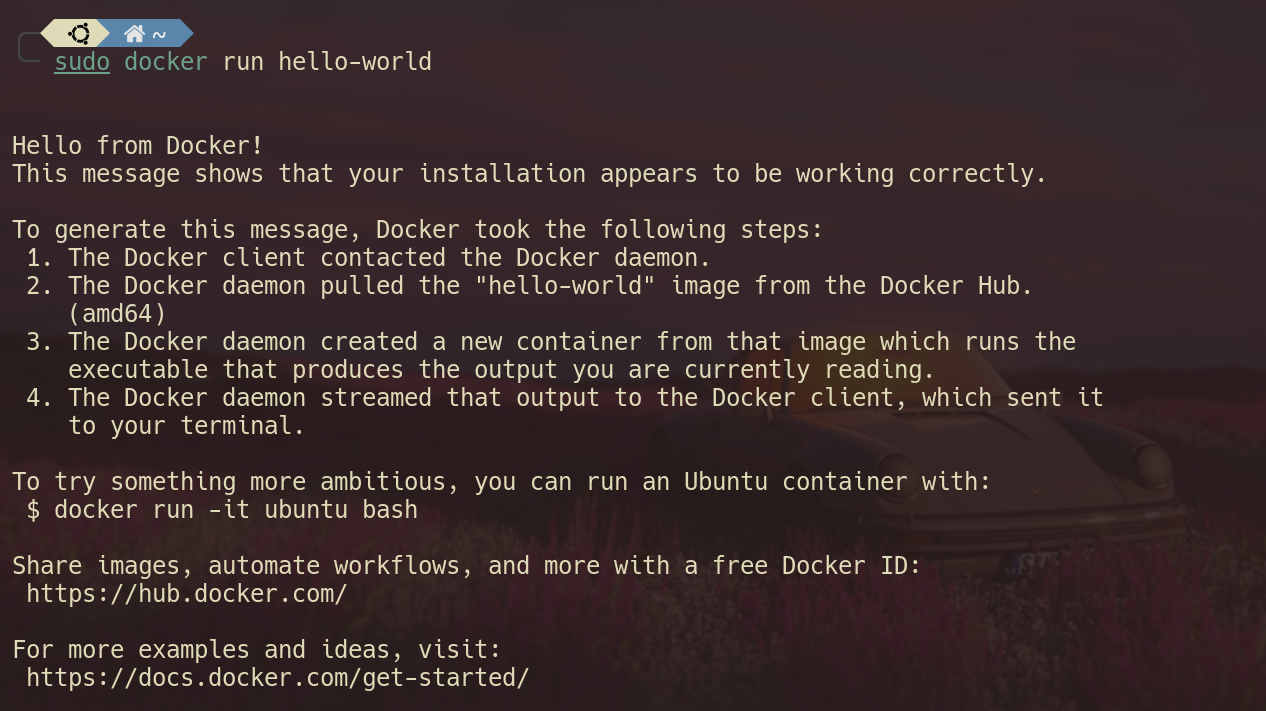
\includegraphics[width=0.6\textwidth]{images/Bloque2/hello-world.png}
    \caption{Contenedor Hello World}
    \label{fig:hello-world}
\end{figure}

\section{BenchMarks}

\subsection{¿Qué es un Benchmark?}

Un \textit{benchmark} es una prueba diseñada para medir el rendimiento de un sistema, componente o servicio informático. Estas pruebas pueden evaluar diversos aspectos, como velocidad, eficiencia, capacidad de respuesta o consumo de recursos. Existen múltiples tipos de \textit{benchmarks}, cada uno enfocado en un área específica del sistema.

Por ejemplo, para evaluar el rendimiento de un servidor DNS (que traduce nombres de dominio a direcciones IP), se pueden utilizar herramientas como \texttt{NameBench} o \texttt{GRC’s DNS Benchmark}, las cuales están diseñadas con pruebas estándar para este tipo de servicio.

\subsection{¿Por qué crear un Benchmark propio?}

Aunque existen herramientas predefinidas para realizar \textit{benchmarks}, en ocasiones es necesario programar uno propio para analizar parámetros específicos que no estén cubiertos por las herramientas existentes. Para ello, es importante considerar los siguientes elementos:

\begin{itemize}
    \item \textbf{Objetivo del Benchmark:} Definir claramente qué se desea medir, como latencia, \textit{throughput}, uso de CPU, etc.
    \item \textbf{Métricas:} Establecer las medidas que se utilizarán para evaluar el rendimiento. Esto incluye:
    \begin{itemize}
        \item Las unidades de medida (por ejemplo, milisegundos, MB/s).
        \item Las variables a observar (por ejemplo, tiempo de respuesta, carga del sistema).
        \item El método para calcular los resultados finales.
    \end{itemize}
    \item \textbf{Instrucciones de uso:} Especificar cómo ejecutar el \textit{benchmark}, el entorno requerido y los parámetros necesarios.
    \item \textbf{Ejemplo de uso y análisis de resultados:} Incluir una prueba real, interpretar los datos obtenidos y extraer conclusiones relevantes.
\end{itemize}

\subsection{OpenBenchmarking y Phoronix Test Suite (PTS)}

\subsubsection{OpenBenchmarking}

\textit{OpenBenchmarking} es un repositorio de \textit{benchmarks} de código abierto que permite a los usuarios utilizar, modificar o crear nuevas pruebas basadas en las existentes. Es una excelente fuente de inspiración para desarrollar \textit{benchmarks} personalizados.

\subsubsection{Phoronix Test Suite (PTS)}

\textit{Phoronix Test Suite (PTS)} es una plataforma asociada a \textit{OpenBenchmarking} que facilita la ejecución de \textit{benchmarks}. Es una herramienta versátil y popular para realizar pruebas de rendimiento en sistemas Linux, Windows o incluso en máquinas virtuales (MVs). Entre sus características destacan:

\begin{itemize}
    \item Amplia variedad de pruebas disponibles que se pueden ejecutar directamente desde su entorno.
    \item Integración con \textit{OpenBenchmarking}, lo que permite comparar resultados con otras máquinas.
    \item Compatibilidad con múltiples entornos, incluyendo contenedores Docker.
\end{itemize}

\subsubsection{Instalación de Phoronix Test Suite (PTS)}

La instalación de \textit{PTS} varía según el entorno utilizado:

\begin{itemize}
    \item En sistemas Debian/Ubuntu, se pueden usar paquetes precompilados.
    \item En máquinas virtuales con Rocky Linux, se recomienda el instalador universal para Linux.
    \item En Windows, también se ofrece soporte de instalación.
    \item Para las prácticas, la opción más recomendada es utilizar contenedores Docker.
\end{itemize}

\subsubsection{Enlaces útiles}

A continuación, se presentan enlaces relevantes para explorar más sobre \textit{benchmarks} y herramientas asociadas:

\begin{itemize}
    \item Software relacionado con \textit{benchmarks} en Linux: \\
    \href{https://sourceforge.net/directory/linux/?q=benchmark}{sourceforge.net/directory/linux/?q=benchmark}
    \item Repositorio de OpenBenchmarking: \href{https://openbenchmarking.org/}{openbenchmarking.org}
    \item Sitio web de Phoronix Test Suite: \href{https://www.phoronix-test-suite.com/}{phoronix-test-suite.com}
    \item Página de descargas de PTS: \href{https://www.phoronix-test-suite.com/?k=downloads}{phoronix-test-suite.com/?k=downloads}
    \item Imagen Docker recomendada para las prácticas: \href{https://hub.docker.com/r/phoronix/pts/}{hub.docker.com/r/phoronix/pts/}
\end{itemize}

\subsection{Ejercicio Opcional. Ejecutar un Benchmark}

El alumno/a debe ser capaz de utilizar \textit{Phoronix Test Suite} para:

\begin{itemize}
    \item Descargar, instalar y ejecutar un \textit{benchmark} de su elección.
    \item Almacenar y recuperar los resultados de múltiples ejecuciones del \textit{benchmark}.
    \item Explicar el objetivo del \textit{benchmark} y de los resultados obtenidos.
\end{itemize}

\subsubsection*{Solución con un benchmark distinto}

En mi caso en el propio enlace que nos ofrece la guía\footnote{\url{https://sourceforge.net/directory/linux/?q=benchmark}} he optado por instalar el que benchmarck que tiene como nombre benchmark\footnote{\url{https://sourceforge.net/projects/benchmark.mirror/}} y estoy siguiendo los pasos que aparecen en el fichero \textit{Readme.md}\footnote{Lo estoy instalando en mi máquina anfitrión.}.

Los pasos que he seguido se puede ver en la figura \ref{fig:benchmark}.

\begin{figure}[H]
    \centering
    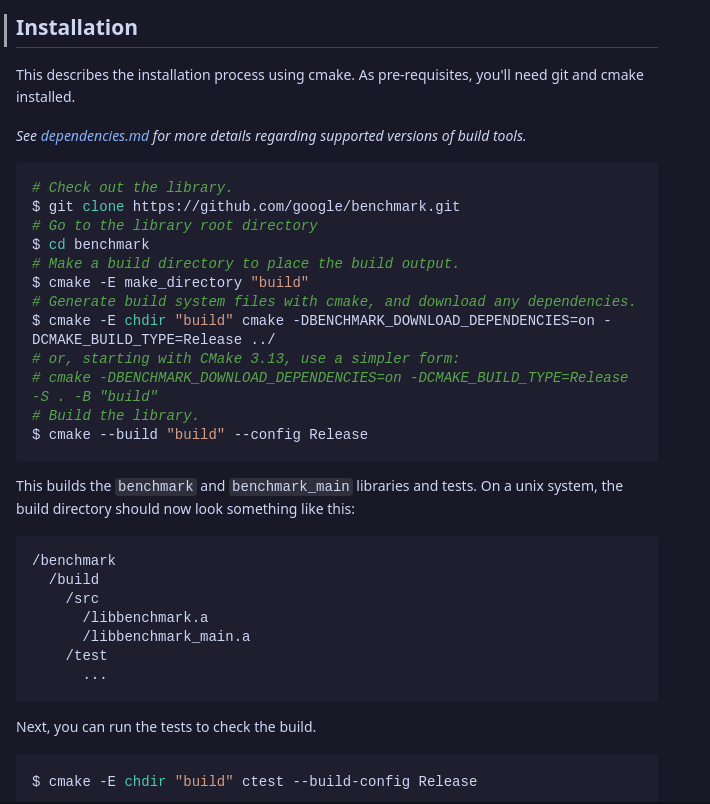
\includegraphics[width=0.6\textwidth]{images/Bloque2/installationBench.png}
    \caption{Instalación de benchmark}
    \label{fig:benchmark}
\end{figure}

Y el resultado del comando de ejecución de los tests lo puede ver en la figura \ref{fig:benchmarkResult}.

\begin{figure}[H]
    \centering
    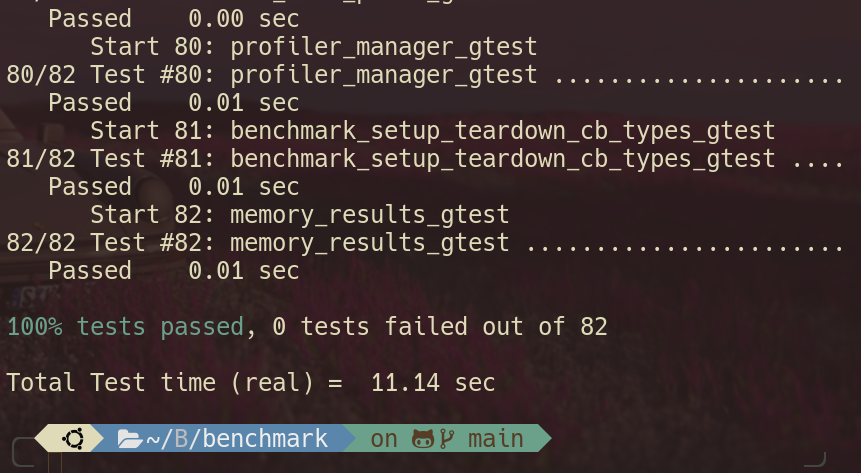
\includegraphics[width=0.6\textwidth]{images/Bloque2/resultsBench.png}
    \caption{Resultado de la ejecución del benchmark}
    \label{fig:benchmarkResult}
\end{figure}

A continuación, instalamos las librerias globales y probamos con el fichero básico que nos proporcioan, compilando y demás, nos da la salida que podemos ver en la figura \ref{fig:benchmarkResult2}.

\begin{figure}[H]
    \centering
    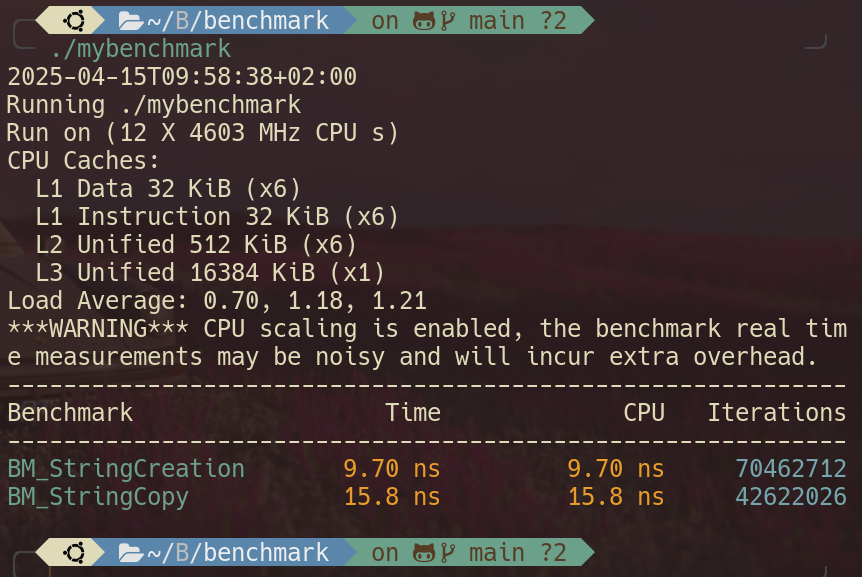
\includegraphics[width=0.6\textwidth]{images/Bloque2/resultsMYBENCHMARK.png}
    \caption{Resultado de la ejecución del benchmark}
    \label{fig:benchmarkResult2}
\end{figure}

\subsection*{Solución usando el benchmark que se especifica}

Para ello me he descargado el zip de la web y como estoy en Linux he ejecutado el comando \micode{sudo ./install.sh} y me ha instalado el programa en la ruta \micode{/usr/bin/phoronix-test-suite}.
\begin{figure}[H]
    \centering
    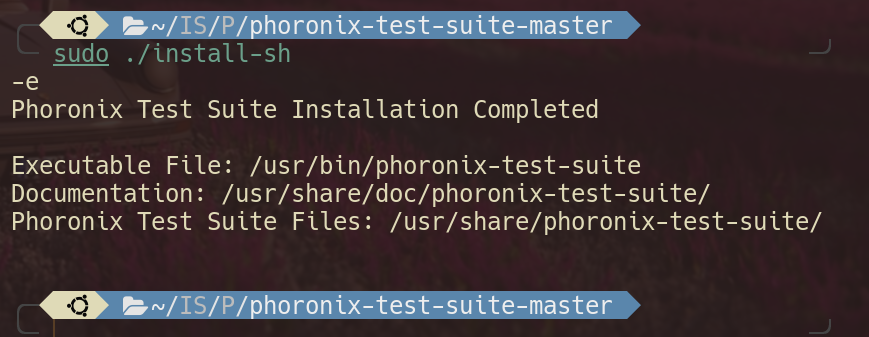
\includegraphics[width=0.6\textwidth]{images/Bloque2/installPhoro.png}
    \caption{Instalación de Phoronix Test Suite}
    \label{fig:PTS}
\end{figure}

Debemos de leer el Readme para una prueba.

En base a \textit{``phoronix-test-suite benchmark smallpt to run a simple CPU test
profile''} introducimos el comando para un primer testeo. 

% \includepdf[nup=2x2, pages=1-3, frame=true]{"../../Ficheros_Ejercicios/Ejercicios_Bloque2/resultsfirststatement.pdf"}

Donde el resultado que nos da:

\begin{lstlisting}
    resultsFirstAttempt
results


results: 

	Processor: AMD Ryzen 5 7535HS @ 4.60GHz (6 Cores / 12 Threads), Motherboard: ASUS TUF Gaming A15 FA506NC_FA506NC FA506NC v1.0 (FA506NC.308 BIOS), Chipset: AMD 17h-19h PCIe Root Complex, Memory: 2 x 8GB DDR5-4800MT/s Samsung M425R1GB4PB0-CWMOL, Disk: 512GB SAMSUNG MZVL8512HELU-00BTW + 1000GB KINGSTON SNV3S1000G, Graphics: ASUS NVIDIA GeForce RTX 3050 Mobile, Audio: NVIDIA Device 2291, Network: Realtek RTL8111/8168/8211/8411 + Realtek RTL8852BE PCIe 802.11ax

	OS: Ubuntu 24.04, Kernel: 6.11.0-21-generic (x86_64), Display Server: X Server, Compiler: GCC 13.3.0, File-System: ext4, Screen Resolution: 1920x1080


Smallpt 1.0
Global Illumination Renderer; 128 Samples
Seconds < Lower Is Better
results . 15.48 |==============================================================

\end{lstlisting}

% Otro de los benchmarks que podemos ejecutar es ``unigine-heaven''. Para ello debemos de ejecutar los comandos \micode{./phoronix-test-suite install unigine-heaven; ./phoronix-test-suite run unigine-heaven}


\subsection{Resumen: Phoronix Test Suite en Máquina Local vs Docker}

El \textit{Phoronix Test Suite} puede presentar problemas de rendimiento o fallos en una máquina local debido a dependencias faltantes, configuraciones incorrectas o conflictos en el entorno del sistema operativo. En contraste, al ejecutarlo en un contenedor Docker, se utiliza un entorno limpio y preconfigurado, optimizado por los desarrolladores para funcionar de manera eficiente.

\subsubsection{Comparativa entre Máquina Local y Docker}

\begin{table}[h!]
\centering
\begin{tabular}{|p{4cm}|p{5cm}|p{5cm}|}
\hline
\textbf{Aspecto} & \textbf{Máquina Local} & \textbf{Contenedor Docker} \\ \hline
PHP y extensiones & Puede faltar GD, bzip2, sqlite3, etc. & Todo preinstalado y configurado \\ \hline
Permisos y acceso a GPU & Problemas con \texttt{/dev/dri} u otros permisos & Aislado, puede no usar GPU directamente \\ \hline
Entorno gráfico & Falta de X11 puede romper tests gráficos & Usa \textit{fallback} o modo \textit{headless} \\ \hline
Dependencias del sistema & Conflictos o paquetes rotos & Imagen oficial limpia y probada \\ \hline
Compatibilidad de librerías & Incompatibilidades posibles & Versiones probadas y compatibles \\ \hline
\end{tabular}
\caption{Comparativa entre ejecución local y en Docker}
\end{table}

\subsubsection{Caso Específico: Benchmark \texttt{smallpt}}

El \texttt{smallpt} es un \textit{benchmark} dependiente de la CPU. Problemas como \textit{throttling}, gestión térmica deficiente o extensiones PHP faltantes pueden ralentizar su ejecución en una máquina local. En Docker, estos problemas se mitigan gracias al entorno controlado.

\subsubsection{Ventajas de Docker}

\begin{itemize}
    \item Entorno aislado y preconfigurado.
    \item Independencia de configuraciones locales.
    \item Fácil reinicio y limpieza del entorno.
    \item Uso de versiones probadas por los desarrolladores.
\end{itemize}

En resumen, ejecutar \textit{Phoronix Test Suite} en Docker garantiza mayor estabilidad y rendimiento, eliminando problemas derivados del entorno local.



Realizando diversas pruevas vemos que el comando tarda demasiado y con htop vemos que no se queda colgado pero tarda demasiado tiempo, por ende, he decidido ejecutarlo en contenedores que es como se recomienda en prácticas. 


Para ello ejecutamos los siguientes comandos:

\begin{enumerate}
    \item \micode{docker pull phoronix/pts}: para descargar la imagen de Phoronix Test Suite\footnote{El comando es de la \url{https://www.phoronix-test-suite.com/?k=downloads}.}.
    \item \micode{docker run -it --rm phoronix/pts}: para ejecutar el contenedor interactivo.
    \item \micode{phoronix-test-suite benchmark smallpt}: para ejecutar el benchmark.
\end{enumerate}

De manera que una vez que estamos dentro de la shell interactiva del docker podemos ejecutar los comandos del docker.

Los pasos a seguir para los tests son (dentro del docker de phoronix con la shell interactiva):
\begin{enumerate}
    \item Listamos los disponibles usando el comando \micode{list-avilable-test}
    \item install <test>
    \item run <test>
\end{enumerate}

En mi caso con he instalado el test \micode{php}. El resultado podemos verlo en la terminal (Ver figura \ref{fig:dockerPhoronix}). Además tenemos la opción de subirlo y poder consultarlo de manera online, en mi caso es \url{https://openbenchmarking.org/result/2504152-NE-RESULTSPH66}.

\begin{figure}[H]
    \centering
    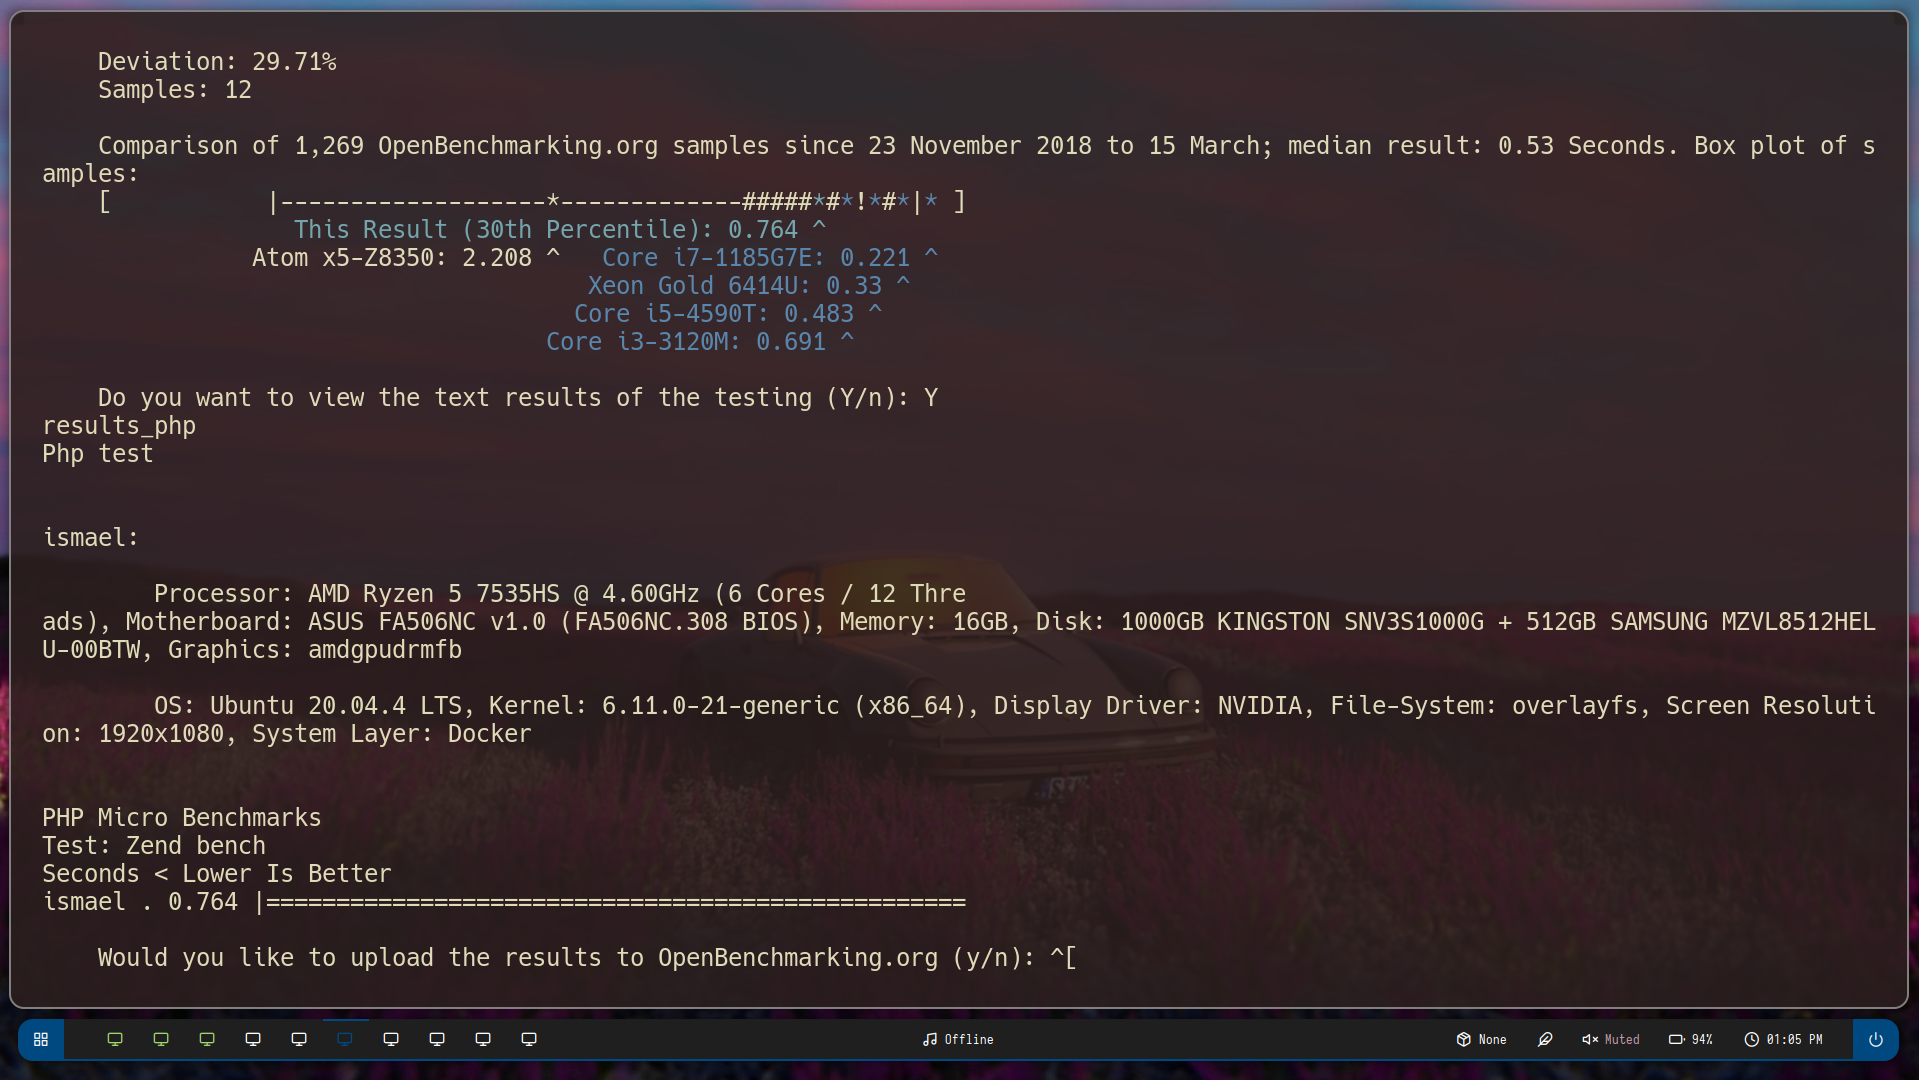
\includegraphics[width=1\textwidth]{images/Bloque2/dockerPhoronix.png}
    \caption{Resultado de la ejecución del benchmark en Docker}
    \label{fig:dockerPhoronix}
\end{figure}

\subsection*{Objetivo del Benchmark y Resultados Obtenidos}

El objetivo del benchmark realizado con \textbf{Phoronix Test Suite} fue evaluar el rendimiento del sistema, específicamente en la ejecución de pruebas micro de \textbf{PHP Zend}, bajo condiciones estándar. Este tipo de pruebas mide la eficiencia y tiempos de ejecución de componentes clave, como el procesador y la memoria, proporcionando una comparación con otros sistemas.

\subsubsection{Resultados Obtenidos}

\begin{itemize}
    \item \textbf{Tiempo promedio de ejecución}: 0.764 segundos.
    \item \textbf{Desviación estándar}: SE +/- 0.066, lo que indica una alta consistencia en los resultados.
    \item \textbf{Percentil alcanzado}: No especificado, pero los resultados muestran un rendimiento competitivo en comparación con sistemas similares.
\end{itemize}

\subsubsection{Interpretación de los Resultados}

El sistema probado, con un procesador AMD Ryzen 5 7535HS, mostró un rendimiento destacado en las pruebas de PHP Zend, con tiempos de ejecución significativamente bajos. Esto lo posiciona como una opción eficiente para entornos que requieren alta velocidad y confiabilidad en la ejecución de aplicaciones web o API basadas en PHP.

\subsubsection{Conclusión}

El benchmark confirma que el sistema es altamente eficiente en tareas relacionadas con PHP, siendo una opción ideal para desarrolladores y administradores de sistemas que buscan optimizar el rendimiento de sus servidores o aplicaciones en entornos de producción.


\subsection{Ejercicio Opcional. Comparar benchmark en contenedor y en VM}

El alumno/a ejecutará el mismo benchmark sobre: su ordenador personal, Docker en su ordenador personal y máquina virtual. Comente y justifique las posibles diferencias en los resultados obtenidos.

\subsubsection{Solución}

\begin{itemize}
    \item En cuanto a ejecutarlo en el Docker de nuestro ordenador personal, el resultado es el que hemos visto en el anterior ejercicio. Podemos ver la figura \ref{fig:dockerPhoronix}.
    \item En cuanto a la parte de ejecutarlo en nuestra máquina, vemos que anteriormente lo habíamos hecho pero tras el intento de mejorar el rendimiento instalando los drivers recomendados para ubuntu de nvidia no funcionaba, por lo que \textcolor{red}{debemos de destacar que se deben de usar los drivers de nouveau (código abierto)}, ya que si no en caso contrario se daban problemas de priorización de programas, kernel, se cuelga la detección del hardware y demás. Generando el comando básico nos quedan los resultados de nuestra máquina en la web: \url{https://openbenchmarking.org/result/2504153-NE-RESULTS0676}. De esta manera ejecutamos los comandos: 
    \begin{enumerate}
        \item \micode{phoronix-test-suite install pts/git}
        \item \micode{phoronix-test-suite run pts/git}
    \end{enumerate}

    \begin{figure}[H]
        \centering
        \begin{minipage}{0.45\textwidth}
            \centering
            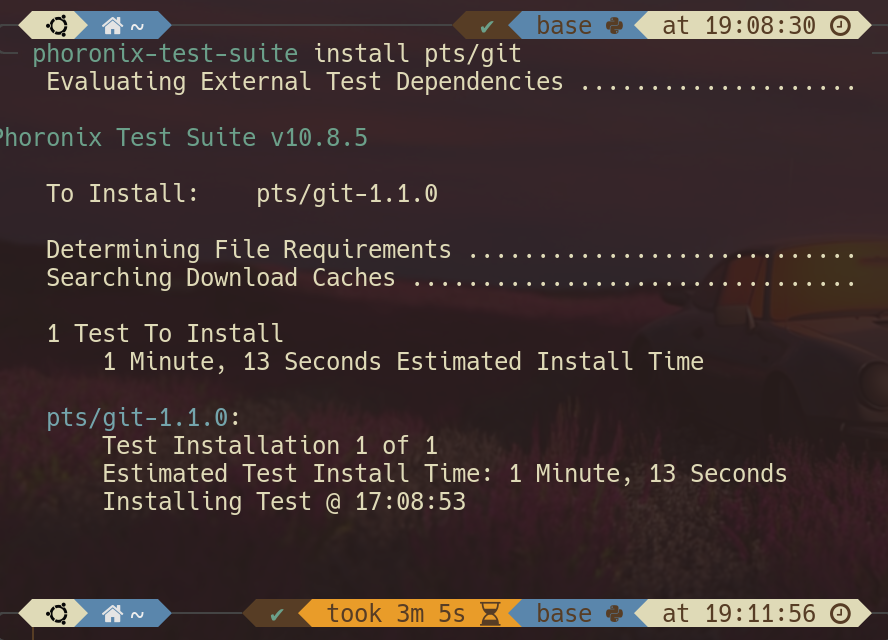
\includegraphics[width=\textwidth]{images/Bloque2/personal-phoronix-1.png}
            \caption{Instalación del test git}
            \label{fig:image1}
        \end{minipage}
        \hfill
        \begin{minipage}{0.45\textwidth}
            \centering
            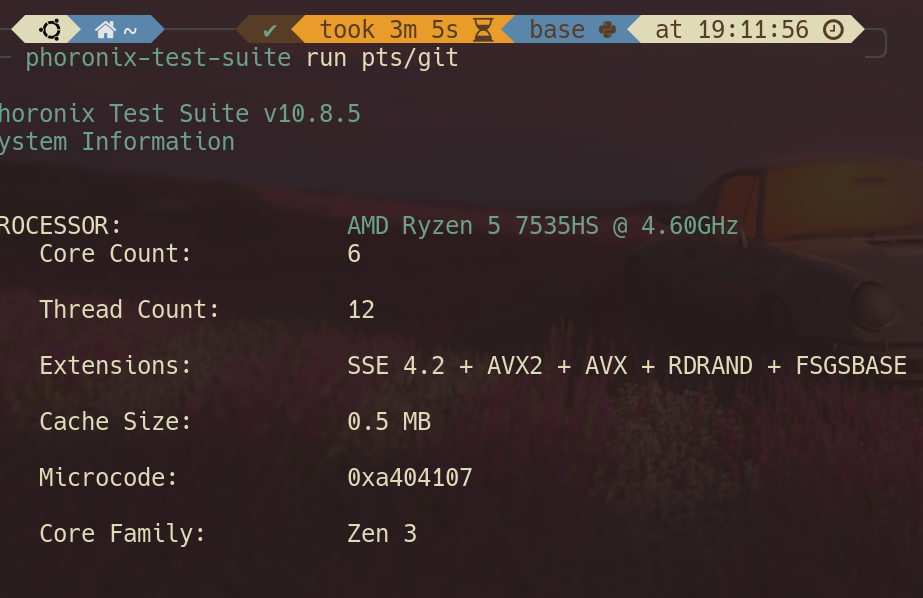
\includegraphics[width=\textwidth]{images/Bloque2/personal-phoronix-2.png}
            \caption{Run del test}
            \label{fig:image2}
        \end{minipage}
    \end{figure}
    \begin{figure}[H]
        \centering
        \begin{minipage}{0.45\textwidth}
            \centering
            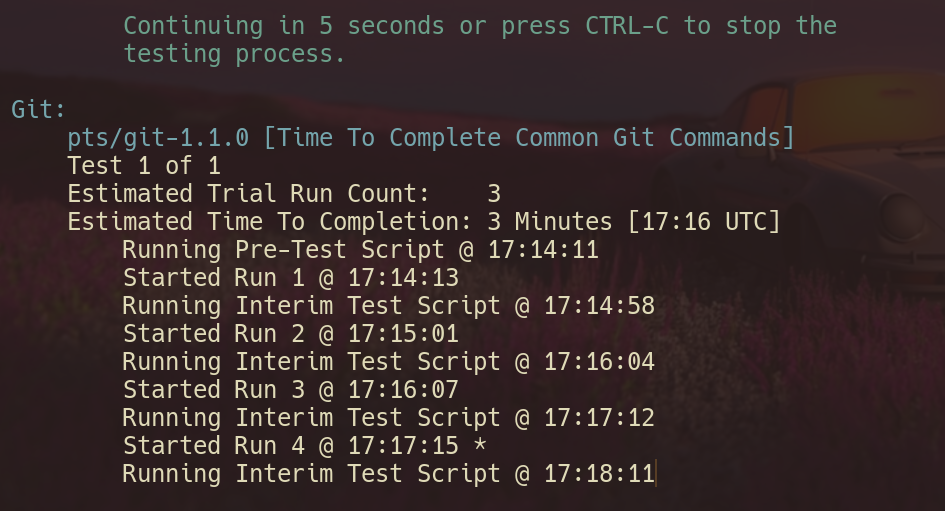
\includegraphics[width=\textwidth]{images/Bloque2/per-pho-3.png}
            \caption{Run del test en ejecución}
            \label{fig:image5}
        \end{minipage}
        \hfill
        \begin{minipage}{0.45\textwidth}
            \centering
            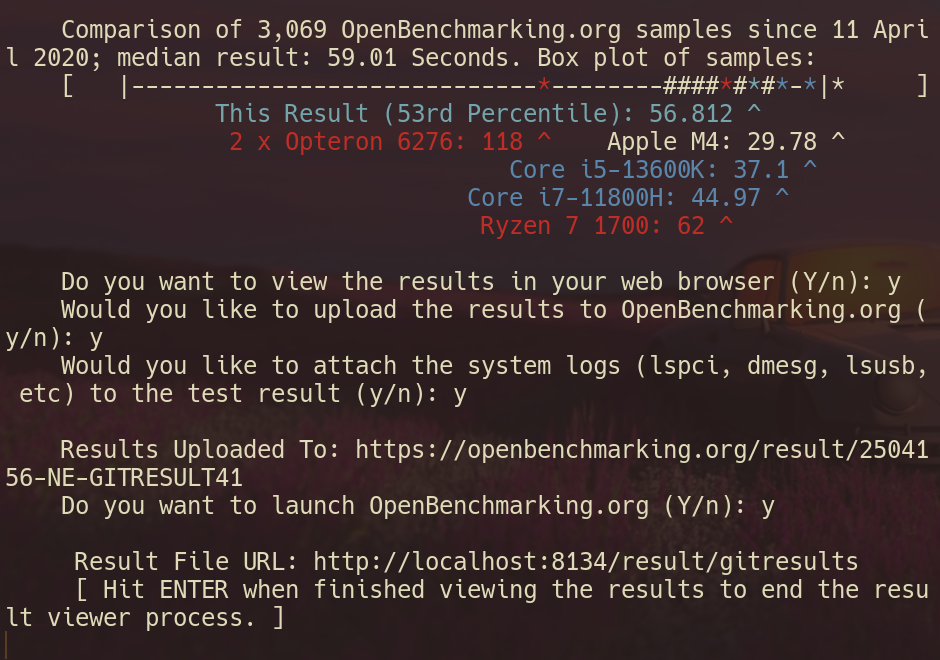
\includegraphics[width=\textwidth]{images/Bloque2/fin-git-pho.png}
            \caption{Run del test}
            \label{fig:image6}
        \end{minipage}
    \end{figure}
    Para acceder a los resultados podemos acceder al enlace: \url{https://openbenchmarking.org/result/2504156-NE-GITRESULT41}.
    \item En el caso de la máquina virtual, en mi caso he clonado la última y he cambiado de nuevo la ip. Para la descarga de phoronix podemos usar curl, wget pero yo he usado scp desde mi máquina local: \micode{scp -r Descargas/phoronix-test-suite-master ismMV01@192.168.56.106:~} (Debemos pasarlo unzipeado debido a que no tenemos la herramienta unzip).
    \begin{figure}[H]
        \centering
        \begin{minipage}{0.45\textwidth}
            \centering
            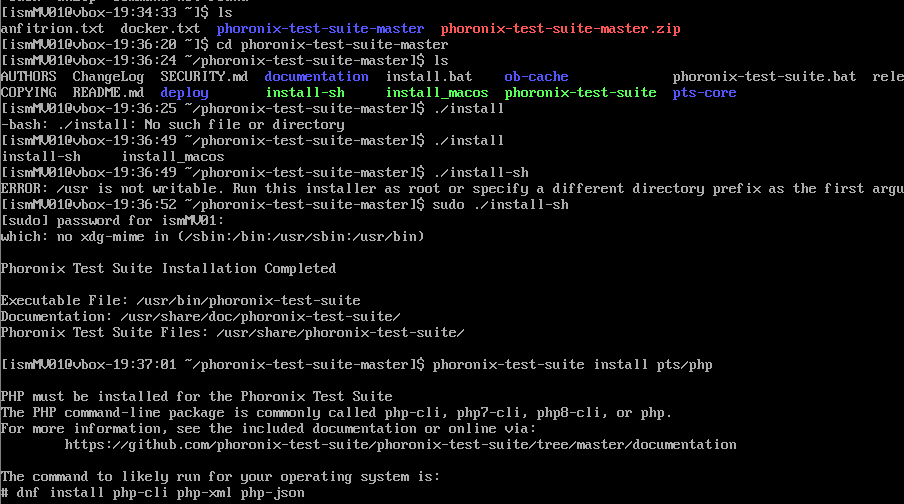
\includegraphics[width=\textwidth]{images/Bloque2/mv-pho-1.png}
            \caption{Instalaciónd de phoronix en MV Rocky, a continuación instalamos lo que nos dice, ya que instalamos pts/php}
            \label{fig:image7}
        \end{minipage}
        \hfill
        \begin{minipage}{0.45\textwidth}
            \centering
            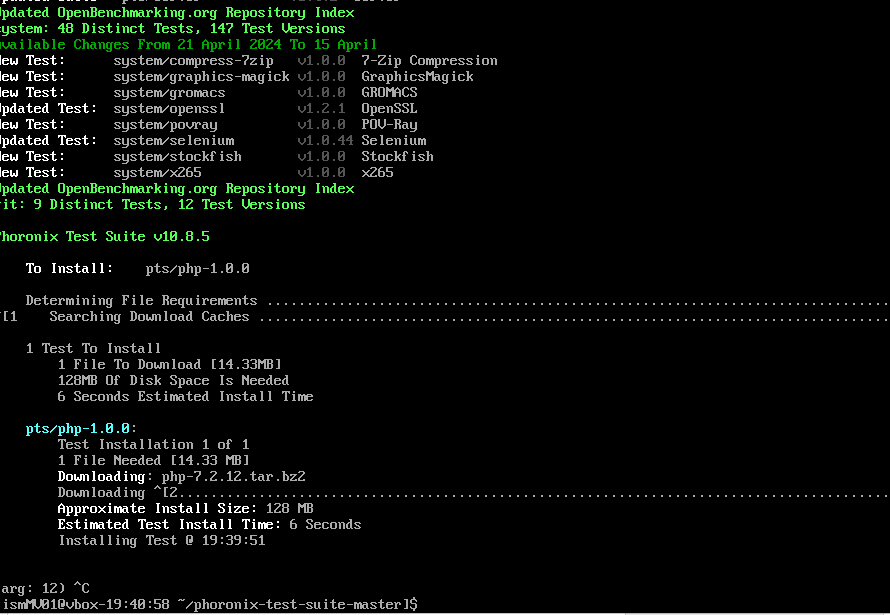
\includegraphics[width=\textwidth]{images/Bloque2/mv-pho-2.png}
            \caption{Install de pts/php}
            \label{fig:image8}
        \end{minipage}
    \end{figure}
    \begin{figure}[H]
        \centering
        \begin{minipage}{0.45\textwidth}
            \centering
            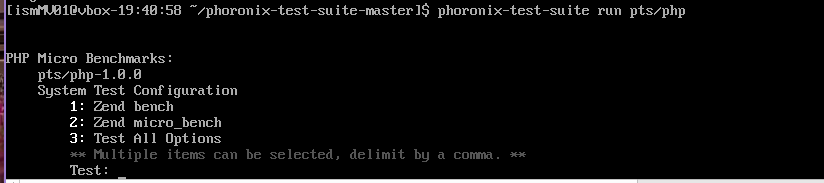
\includegraphics[width=\textwidth]{images/Bloque2/mv-pho-4.png}
            \caption{Ejecutamos el test}
            \label{fig:image9}
        \end{minipage}
        \hfill
        \begin{minipage}{0.45\textwidth}
            \centering
            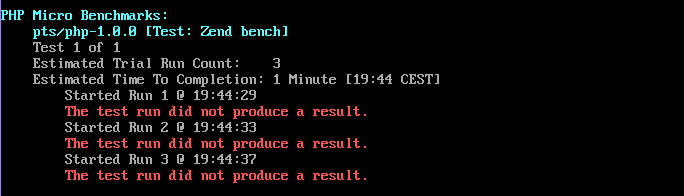
\includegraphics[width=\textwidth]{images/Bloque2/mv-pho-5.png}
            \caption{Resultado final (Vemos que no se generan resultados)}
            \label{fig:image10}
        \end{minipage}
    \end{figure}
    
\end{itemize}



\subsection{Apache Benchmarck}


\texttt{Apache Benchmark (ab)} es una herramienta de línea de comandos incluida en el servidor web Apache, diseñada para medir el rendimiento de servidores HTTP. Es especialmente útil para realizar pruebas de carga y evaluar la capacidad de respuesta de un servidor bajo diferentes niveles de tráfico.

\subsubsection{Instalación}

En la mayoría de las distribuciones Linux, \texttt{ab} se incluye como parte del paquete \texttt{apache2-utils}. Para instalarlo, ejecute:

\begin{lstlisting}[style=customstyle]
sudo apt install apache2-utils -y
\end{lstlisting}

\subsubsection{Uso Básico}

El comando básico para ejecutar \texttt{ab} es:

\begin{lstlisting}[style=customstyle]
ab -n <número_de_peticiones> -c <concurrencia> <URL>
\end{lstlisting}

\begin{itemize}
    \item \texttt{-n}: Número total de peticiones a realizar.
    \item \texttt{-c}: Número de peticiones concurrentes.
    \item \texttt{<URL>}: \\
    Dirección completa del recurso a probar (por ejemplo, \texttt{http://localhost/index.html}).
\end{itemize}

\subsubsection{Ejemplo de Uso}

Para realizar 100 peticiones con una concurrencia de 10 al servidor local, ejecute:

\begin{lstlisting}[style=customstyle]
ab -n 100 -c 10 http://localhost/
\end{lstlisting}

\subsubsection{Resultados}

El comando genera un informe detallado con métricas clave, como:

\begin{itemize}
    \item \textbf{Tiempo total de prueba:} Duración total de la prueba en segundos.
    \item \textbf{Peticiones por segundo:} Número promedio de peticiones procesadas por segundo.
    \item \textbf{Tiempo de respuesta promedio:} Tiempo promedio que tarda el servidor en responder a una petición.
    \item \textbf{Transferencia por segundo:} Cantidad de datos transferidos por segundo.
\end{itemize}

\subsubsection{Consideraciones}

\begin{itemize}
    \item \texttt{ab} no soporta HTTPS de forma nativa en algunas versiones. Para pruebas HTTPS, considere herramientas alternativas como \texttt{wrk} o \texttt{siege}.
    \item Asegúrese de que el servidor pueda manejar la carga generada por \texttt{ab} para evitar resultados poco representativos.
\end{itemize}

\subsubsection{Resumen}

\texttt{Apache Benchmark} es una herramienta sencilla pero poderosa para realizar pruebas de rendimiento en servidores HTTP. Su facilidad de uso y disponibilidad la convierten en una opción ideal para desarrolladores y administradores de sistemas que buscan evaluar la capacidad de sus servidores.

\subsection{Ejercicio Opcional. Carga Http con AB}

Ejecute el benchmark sobre los servidores Http empleados en las prácticas del Bloque 1 (Apache y Nginx). Se deja a la decisión del alumno/a la definición de los parámetros del benchmark, pero se valorará que sea capaz de definir un entorno de ejecución que eleve significativamente la carga de los servidores. El alumno/a debe ser capaz de describir en detalle los resultados obtenidos así como razonar las posibles diferencias entre los servidores.


\subsubsection{Solución}

Para hacerlo más fácil he decidido hacerlo desde un contenedor de docker en mi máquina local, los pasos son:

\begin{enumerate}
    \item Creamos el directorio donde vamos a crear el fihero docker-compose.yml y donde vamos a trabajar.
    \item Editamos el fichero \micode{docker-compose.yml} y le añadimos el siguiente contenido:
    \begin{lstlisting}[style=customstyle]
    version: '3'  # Versión del archivo docker-compose

    services:
        apache:  # Servicio para el servidor Apache
            image: httpd:2.4  # Imagen de Docker para Apache HTTP Server versión 2.4
            container_name: apache-server  # Nombre del contenedor para Apache
            ports:
                - "8080:80"  # Mapea el puerto 80 del contenedor al puerto 8080 del host

        nginx:  # Servicio para el servidor Nginx
            image: nginx:alpine  # Imagen de Docker para Nginx basada en Alpine Linux
            container_name: nginx-server  # Nombre del contenedor para Nginx
            ports:
                - "8081:80"  # Mapea el puerto 80 del contenedor al puerto 8081 del host

        ab:  # Servicio para Apache Benchmark (ab)
            image: jordi/ab  # Imagen de Docker que contiene Apache Benchmark
            container_name: ab-client  # Nombre del contenedor para Apache Benchmark
            entrypoint: tail -f /dev/null  # Mantiene el contenedor en ejecución para usarlo con `docker exec`
        \end{lstlisting}
        \item Guardamos el fichero y ejecutamos el siguiente comando para levantar los contenedores: \micode{docker-compose up -d}.
        \item Vemos que efectivamente están corriendo: \micode{docker ps}.
        \item Accedemos al contenedor de ab: \micode{docker exec -it ab-client sh}.
        \item Dentro de la shell interactiva ejecutamos los comandos:
        \begin{enumerate}
            \item \micode{ab -n 1000 -c 50 http://apache-server/ > apache.txt}: para ejecutar el benchmark en el servidor Apache y guardar los resultados en un archivo llamado \texttt{apache.txt}.
            \item \micode{ab -n 1000 -c 50 http://nginx-server/ > nginx.txt}: para ejecutar el benchmark en el servidor Nginx y guardar los resultados en un archivo llamado \texttt{nginx.txt}.
        \end{enumerate}
        \item Copiamos el contenido del contedor (este comando se ejecuta desde nuestra máquina local, no dentro del contenedor): \micode{docker cp ab-client:/apache.txt ./apache.txt ; 
        docker cp ab-client:/nginx.txt ./nginx.txt}
\end{enumerate}

En cuanto a interpretar los resultados, solo vamos a hacer el fichero \micode{apache.txt}: 

\subsubsection*{Análisis en profundidad de los resultados}

El objetivo principal del benchmark realizado con \textbf{ApacheBench (ab)} es medir el rendimiento del servidor HTTP Apache bajo condiciones de carga. Esto incluye evaluar:

\begin{itemize}
    \item \textbf{Capacidad de manejo de peticiones:} Cuántas solicitudes por segundo puede procesar el servidor.
    \item \textbf{Latencia:} Tiempo promedio de respuesta por petición.
    \item \textbf{Estabilidad:} Cómo se comporta el servidor con múltiples clientes concurrentes.
\end{itemize}

\paragraph{Información Básica del Servidor}

\begin{table}[H]
\centering
\begin{tabular}{|p{5cm}|p{5cm}|p{5cm}|}
\hline
\textbf{Campo} & \textbf{Valor} & \textbf{Explicación} \\ \hline
\textbf{Server Software} & Apache/2.4.63 & Versión del servidor Apache \\ \hline
\textbf{Hostname} & apache-server & Nombre del servidor bajo prueba \\ \hline
\textbf{Port} & 80 & Puerto HTTP estándar \\ \hline
\textbf{Document Path} & / & Página que se está solicitando (raíz) \\ \hline
\textbf{Document Length} & 45 bytes & Tamaño del contenido HTML que responde el servidor \\ \hline
\end{tabular}
\caption{Información básica del servidor}
\end{table}

\paragraph{Parámetros de Prueba}

\begin{table}[H]
\centering
\begin{tabular}{|p{5cm}|p{5cm}|p{5cm}|}
\hline
\textbf{Campo} & \textbf{Valor} & \textbf{Explicación} \\ \hline
\textbf{Concurrency Level} & 50 & Simulación de 50 clientes simultáneos \\ \hline
\textbf{Complete Requests} & 1000 & Total de peticiones realizadas al servidor \\ \hline
\textbf{Failed Requests} & 0 & Todas las solicitudes fueron exitosas \\ \hline
\end{tabular}
\caption{Parámetros de prueba}
\end{table}

\paragraph{Rendimiento del Servidor}

\begin{table}[H]
\centering
\begin{tabular}{|p{5cm}|p{5cm}|p{5cm}|}
\hline
\textbf{Campo} & \textbf{Valor} & \textbf{Explicación} \\ \hline
\textbf{Time taken for tests} & 0.165 s & Tiempo total de la prueba \\ \hline
\textbf{Requests per second} & 6057.60 req/s & Rendimiento: peticiones procesadas por segundo \\ \hline
\textbf{Time per request (mean)} & 8.254 ms & Tiempo promedio por petición individual \\ \hline
\textbf{Time per request (concurrent)} & 0.165 ms & Tiempo promedio por petición con concurrencia \\ \hline
\textbf{Transfer rate} & 1709.61 KB/s & Velocidad de transferencia promedio \\ \hline
\end{tabular}
\caption{Rendimiento del servidor}
\end{table}

\paragraph{Tiempos de Conexión y Procesamiento}

\begin{table}[H]
\centering
\begin{tabular}{|p{2cm}|p{2cm}|p{2cm}|p{2cm}|p{2cm}|p{2cm}|}
\hline
\textbf{Tipo} & \textbf{min} & \textbf{mean} & \textbf{sd} & \textbf{med} & \textbf{max} \\ \hline
\textbf{Connect} & 0 ms & 4 ms & ±1.2 & 3 ms & 8 ms \\ \hline
\textbf{Processing} & 1 ms & 4 ms & ±1.3 & 4 ms & 10 ms \\ \hline
\textbf{Waiting} & 0 ms & 3 ms & ±1.2 & 3 ms & 8 ms \\ \hline
\textbf{Total} & 4 ms & 8 ms & ±1.7 & 8 ms & 13 ms \\ \hline
\end{tabular}
\caption{Tiempos de conexión y procesamiento}
\end{table}

\paragraph{Distribución de Latencias}

\begin{table}[H]
\centering
\begin{tabular}{|l|l|}
\hline
\textbf{Percentil} & \textbf{Tiempo} \\ \hline
50\% (mediana) & 8 ms \\ \hline
66\% & 9 ms \\ \hline
75\% & 9 ms \\ \hline
90\% & 11 ms \\ \hline
100\% (máxima) & 13 ms \\ \hline
\end{tabular}
\caption{Distribución de latencias}
\end{table}


\begin{itemize}
    \item El servidor Apache demostró un rendimiento excelente, procesando más de \textbf{6000 peticiones por segundo} sin errores.
    \item La \textbf{latencia es baja y estable}, con tiempos de respuesta promedio de 8 ms y una variabilidad mínima.
    \item La distribución de latencias muestra que el \textbf{99\% de las peticiones} se completaron en 12 ms o menos, lo que indica un comportamiento altamente eficiente.
\end{itemize}

\section{Simulación de Carga con Jmeter}

\subsection{Comparativa de herramientas de pruebas de carga y rendimiento}

Existen diversas herramientas para realizar pruebas de carga y rendimiento, cada una con características específicas que las hacen más adecuadas para ciertos escenarios. A continuación, se presenta una comparación de las herramientas más populares:

\subsubsection{Apache JMeter}

Apache JMeter es una herramienta de código abierto desarrollada en Java por la Apache Software Foundation. Es ampliamente utilizada para pruebas de carga y rendimiento en aplicaciones web, bases de datos, servicios web, entre otros.

\textbf{Características principales:}
\begin{itemize}
    \item Soporte para múltiples protocolos: HTTP, FTP, JDBC, LDAP, JMS, entre otros.
    \item Permite ejecutar pruebas en modo gráfico o desde la línea de comandos, facilitando la integración en pipelines de CI/CD.
    \item Capacidad de distribuir la carga entre múltiples máquinas para simular un gran número de usuarios concurrentes.
    \item Integración con Selenium para pruebas funcionales.
\end{itemize}

\subsubsection{Flood.io (Tricentis Flood)}

Flood.io es una plataforma SaaS que permite ejecutar pruebas de carga distribuidas globalmente utilizando herramientas de código abierto como JMeter, Gatling y Selenium.

\textbf{Características principales:}
\begin{itemize}
    \item Ejecución de pruebas desde múltiples ubicaciones geográficas sin necesidad de configurar infraestructura adicional.
    \item Soporte para scripts escritos en Ruby JMeter y Flood Element (basado en TypeScript).
    \item Integración con servicios en la nube como AWS y Azure.
    \item Generación de informes detallados y monitoreo en tiempo real.
\end{itemize}

\subsubsection{Gatling}

Gatling es una herramienta de pruebas de carga y rendimiento escrita en Scala, Akka y Netty. Está diseñada para ser eficiente en el uso de recursos y permite simular un gran número de usuarios desde una sola máquina.

\textbf{Características principales:}
\begin{itemize}
    \item Uso de un lenguaje específico de dominio (DSL) para definir escenarios de prueba de manera legible y mantenible.
    \item Generación automática de informes HTML con métricas detalladas.
    \item Soporte para protocolos como HTTP, WebSockets, JMS, entre otros.
    \item Integración con herramientas de CI/CD y entornos de desarrollo.
\end{itemize}

\subsubsection{Locust}

Locust es una herramienta de pruebas de carga escrita en Python que permite definir escenarios de usuario utilizando scripts en este lenguaje.

\textbf{Características principales:}
\begin{itemize}
    \item Facilidad para escribir y mantener scripts de prueba gracias al uso de Python.
    \item Interfaz web para monitorear y controlar las pruebas en tiempo real.
    \item Capacidad de distribuir la carga entre múltiples máquinas o procesos.
    \item Soporte para protocolos como HTTP, gRPC, WebSockets, entre otros, mediante plugins.
\end{itemize}

\subsubsection{K6}

K6 es una herramienta de pruebas de carga de código abierto desarrollada por Grafana Labs. Está escrita en Go y utiliza JavaScript para definir los scripts de prueba.

\textbf{Características principales:}
\begin{itemize}
    \item Facilidad de uso para desarrolladores gracias al uso de JavaScript.
    \item Integración con pipelines de CI/CD para pruebas automatizadas.
    \item Soporte para diferentes tipos de pruebas: estrés, carga, duración, entre otras.
    \item Posibilidad de visualizar métricas en tiempo real utilizando Grafana.
\end{itemize}

\subsubsection{Artillery}

Artillery es una herramienta de pruebas de carga y rendimiento escrita en Node.js. Permite definir escenarios de prueba utilizando archivos YAML o scripts en JavaScript.

\textbf{Características principales:}
\begin{itemize}
    \item Facilidad para definir escenarios complejos de usuario.
    \item Soporte para pruebas de APIs y aplicaciones web en tiempo real.
    \item Integración con herramientas de CI/CD.
    \item Generación de informes detallados con métricas clave.
\end{itemize}

\subsubsection{Comparativa rápida}

\begin{table}[H]
\centering
\begin{tabular}{|p{3cm}|p{3cm}|p{3cm}|p{3cm}|p{3cm}|}
\hline
\textbf{Herramienta} & \textbf{Lenguaje de scripting} & \textbf{Interfaz gráfica} & \textbf{Distribución de carga} & \textbf{Protocolos soportados} \\ \hline
JMeter & Java & Sí & Sí & HTTP, FTP, JDBC, etc. \\ \hline
Flood.io & Ruby, TypeScript & Sí & Sí (en la nube) & HTTP, Selenium \\ \hline
Gatling & Scala, Java, JS & Parcial & Sí & HTTP, WebSockets \\ \hline
Locust & Python & Sí & Sí & HTTP, gRPC, etc. \\ \hline
K6 & JavaScript & No & Sí & HTTP, WebSockets \\ \hline
Artillery & JavaScript, YAML & No & Sí & HTTP, WebSockets \\ \hline
\end{tabular}
\caption{Comparativa de herramientas de pruebas de carga y rendimiento}
\end{table}

\subsection{Instalación de Jmeter}

\textit{Nota:} en cuanto a la instalación de Jmeter, lo haremos en nuestra máquina local.

Para la instalación debemos de clonar el repositorio \url{https://github.com/davidPalomar-ugr/iseP4JMeter.git} y acto seguido entramos y lanzamos el docker (podemos usar -d para que sea en segundo plano) con el comando: \micode{docker compose up -d}.

\subsection{Detalles sobre el Dockerfile y Docker-Compose}

El \texttt{Dockerfile} es el archivo donde se especifican todos los comandos necesarios para crear una imagen de Docker y las acciones que debe realizar sobre esta, como copiar archivos, instalar paquetes o modificar configuraciones. Desde un punto de vista abstracto, podríamos considerarlo como un \textit{playbook} que Docker aplica al levantar el contenedor.

En este caso, dos elementos clave en el \texttt{Dockerfile} son la configuración del contenedor en lo que respecta a red y almacenamiento. A continuación, se describen los \texttt{Dockerfiles} utilizados en los contenedores de la aplicación y la base de datos:

\subsubsection{Dockerfile de la aplicación (Node.js)}


\begin{lstlisting}[language=Dockerfile]
FROM node:16.13.0-stretch
RUN mkdir -p /usr/src/app
COPY . /usr/src/app
EXPOSE 3000
WORKDIR /usr/src/app
RUN ["npm", "install"]
ENV NODE_ENV=production
CMD ["npm","start"]
\end{lstlisting}

En este archivo:
\begin{itemize}
    \item Se utiliza la imagen base \texttt{node:16.13.0-stretch}, que incluye Node.js versión 16.13.0 y Debian Stretch como sistema operativo.
    \item Se crea un directorio para la aplicación y se copian los archivos del repositorio al contenedor.
    \item Se expone el puerto \texttt{3000}, que será mapeado al puerto del anfitrión.
    \item Se configura la variable de entorno \texttt{NODE\_ENV} como \texttt{production}.
    \item Finalmente, se ejecuta el comando \texttt{npm start} para iniciar la aplicación.
\end{itemize}

\subsubsection{Dockerfile de la base de datos (MongoDB)}

\begin{lstlisting}[language=Dockerfile]
FROM mongo:6
COPY ./scripts/* /tmp/
RUN chmod 755 /tmp/initializeMongoDB.sh
WORKDIR /tmp
CMD ./initializeMongoDB.sh
\end{lstlisting}

En este archivo:
\begin{itemize}
    \item Se utiliza la imagen base \texttt{mongo:6}.
    \item Se copian los scripts necesarios al contenedor y se ajustan los permisos.
    \item Se establece el directorio de trabajo en \texttt{/tmp}.
    \item Finalmente, se ejecuta un script para inicializar y rellenar la base de datos.
\end{itemize}

\subsubsection{Archivo \texttt{docker-compose.yml}}

La herramienta \texttt{docker-compose} permite configurar varios contenedores para que trabajen juntos como un único servicio. El archivo \texttt{docker-compose.yml} especifica los siguientes elementos:



\begin{lstlisting}[language=yaml]
version: '2.0'
services:
  # MongoDB based in the original Mongo Image
  mongodb:
    image: mongo:6
    ports:
      - "27017:27017"
  # Initialize mongodb with data
  mongodbinit:
    build: ./mongodb
    links:
      - mongodb
  # Nodejs App
  nodejs:
    build: ./nodejs
    ports:
      - "3000:3000"
    links:
      - mongodb
\end{lstlisting}

En este archivo:
\begin{itemize}
    \item Se define un servicio para MongoDB, exponiendo el puerto \texttt{27017}.
    \item Se configura un servicio para inicializar MongoDB con datos, que depende del contenedor \texttt{mongodb}.
    \item Se define un servicio para la aplicación Node.js, exponiendo el puerto \texttt{3000} y enlazándolo con el contenedor \texttt{mongodb}.
\end{itemize}

\begin{figure}[H]
    \centering
    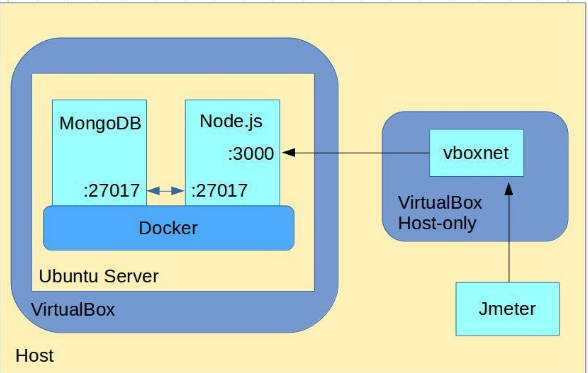
\includegraphics[width=0.6\textwidth]{images/Bloque2/abs-jmeter.png}
    \caption{Descripción de los niveles de abstracción y los distintos elementos en ejecución.}
    \label{fig:docker-compose}
\end{figure}

Esta configuración permite que los contenedores trabajen en conjunto, utilizando la red \texttt{bridge} de Docker para comunicarse entre ellos. Para más detalles, consulte la documentación oficial de Docker y Docker Compose.

\subsection{Ejercicio Obligatorio. Simulación de Carga Http con JMeter}

El repositorio \url{https://github.com/davidPalomar-ugr/iseP4JMeter.git} contiene la aplicación objeto de la prueba de carga y una descripción de los requerimientos sobre la carga a simular. Siga las instrucciones y elabore la prueba de carga con JMeter.

El alumno/a deberá realizar todo el ejercicio en un directorio que contendrá todos los artefactos necesarios para la ejecución de la prueba de carga con JMeter. Dentro de la prueba de carga, los paths a los archivos se definirán de forma relativa para que la ejecución sea independiente de la localización del directorio. Como validación final, el alumno/a debe ser capaz de ejecutar la prueba de carga por línea de comandos (sin interfaz gráfica) desde cualquier directorio de su equipo.

\subsubsection*{Solución}

Para ejecutarlo mediante la línea de comandos sin interfaz gráfica:
\begin{lstlisting}[style=customstyle]
    ./jmeter -n -t /ruta/completa/a/tu/archivo.jmx -l /ruta/completa/a/tu/archivo_resultados.jtl
\end{lstlisting}

\begin{enumerate}
    \item Primero he instalado lo que se conoce como Apache Jmeter, que es una herramienta de pruebas de carga y rendimiento. Para ello he usado el siguiente comando:
    \begin{enumerate}
        \item \micode{wget https://dlcdn.apache.org//jmeter/binaries/apache-jmeter-5.6.3.tgz}
        \item \micode{tar -xvzf apache-jmeter-5.6.3.tgz}
        \item \micode{mv apache-jmeter-5.6.3 ~/jmeter}
    \end{enumerate}
    Y para ejecutarlo:
    \begin{itemize}
        \item Interfaz gráfica: \micode{cd ~/jmeter/bin ; ./jmeter}
        \item Para la línea de comandos: \micode{./jmeter -n -t ruta/al/archivo.jmx -l resultados.jtl -j log.log}
    \end{itemize}
    Para poder lanzar \textit{Jmeter} desde cualquier directorio vamos a añadirlo al path:
    \begin{enumerate}
        \item Abre tu archivo de configuración del shell (por ejemplo \texttt{~/.bashrc} o \texttt{~/.zshrc}):
        \begin{lstlisting}[style=customstyle]
    nano ~/.bashrc
        \end{lstlisting}
        \item Agrega al final:
        \begin{lstlisting}[style=customstyle]
    export PATH="$PATH:$HOME/jmeter/bin"
        \end{lstlisting}
        \item Aplica los cambios:
        \begin{lstlisting}[style=customstyle]
    source ~/.bashrc
        \end{lstlisting}
    \end{enumerate}

    Ahora puedes lanzar \texttt{jmeter} desde cualquier directorio.

    \item Tras clonar el respositorio y demás, creamos un directorio para entregar, para ello ejecutamos el comando: \texttt{mkdir -p jmeter\_test/\{scripts,data,results,logs\}}  
    \item A continuación debemos de ir añadiendo lo necesario para crear el fichero \texttt{.jmx} que queda de la siguiente manera:
    \begin{enumerate}
            \item \textbf{Parametrización de HOST y PUERTO.} \\
            Definimos las variables \texttt{HOST} y \texttt{PORT} para facilitar la configuración del test. Esto se realiza en el Plan de Pruebas: \texttt{Editar $\rightarrow$ Añadir $\rightarrow$ Configuración $\rightarrow$ Variables de Usuario}.

            \item \textbf{Creación del grupo de hebras para los alumnos.} \\
            Creamos un grupo de hebras con 3 usuarios para simular las peticiones de los alumnos. Para ello, en el Plan de Pruebas: \texttt{Editar $\rightarrow$ Añadir $\rightarrow$ Hilos (Usuarios) $\rightarrow$ Grupo de Hilos}.

            \item \textbf{Añadir la petición de acceso al servidor.} \\
            Configuramos los valores por defecto para las peticiones HTTP, haciendo referencia a las variables \texttt{HOST} y \texttt{PORT}. En el Plan de Pruebas: \texttt{Editar $\rightarrow$ Añadir $\rightarrow$ Configuración $\rightarrow$ Valores por Defecto para Petición HTTP}.

            \item \textbf{Definir la autorización básica a la API.} \\
            Configuramos la autorización básica con los datos proporcionados: \texttt{URL Base: http://\$\{HOST\}:\$\{PORT\}/api/v1/auth/login}, \texttt{Usuario: etsiiApi}, \texttt{Contraseña: laApiDeLaETSIIDaLache}. En el Plan de Pruebas: \texttt{Editar $\rightarrow$ Añadir $\rightarrow$ Configuración $\rightarrow$ Gestor de Autorización HTTP}.

            \item \textbf{Definir las credenciales para los alumnos.} \\
            Indicamos que las credenciales de los alumnos se encuentran en el archivo \texttt{alumnos.csv}, cuyos campos son \texttt{usuario} y \texttt{contraseña}. En el grupo \texttt{Alumnos}: \texttt{Editar $\rightarrow$ Añadir $\rightarrow$ Configuración $\rightarrow$ Configuración del CSV Data Set}.

            \item \textbf{Crear una petición POST para los alumnos.} \\
            Añadimos una petición HTTP para realizar el login de los alumnos. En el grupo \texttt{Alumnos}: \texttt{Editar $\rightarrow$ Añadir $\rightarrow$ Muestreador $\rightarrow$ Petición HTTP}.

            \item \textbf{Recuperar el token de autenticación.} \\
            Configuramos un extractor de expresiones regulares para capturar el token devuelto por el servidor tras una autenticación válida. En \texttt{Login Alumnos}: \texttt{Editar $\rightarrow$ Añadir $\rightarrow$ Post Procesadores $\rightarrow$ Extractor de Expresiones Regulares}.

            \item \textbf{Añadir un temporizador aleatorio.} \\
            Para simular accesos más realistas, añadimos un temporizador que siga una distribución Gaussiana. En el grupo \texttt{Alumnos}: \texttt{Editar $\rightarrow$ Añadir $\rightarrow$ Temporizador $\rightarrow$ Temporizador Aleatorio Gaussiano}.

            \item \textbf{Recuperar los datos de los alumnos.} \\
            Creamos una petición GET para obtener los datos de los alumnos. En el grupo \texttt{Alumnos}: \texttt{Editar $\rightarrow$ Añadir $\rightarrow$ Muestreador $\rightarrow$ Petición HTTP}.

            \item \textbf{Resolver problemas de token inválido.} \\
            Configuramos un gestor de cabecera HTTP para manejar problemas relacionados con la validez del token. En el grupo \texttt{Alumnos}: \texttt{Editar $\rightarrow$ Añadir $\rightarrow$ Configuración $\rightarrow$ Gestor de Cabecera HTTP}.

            \item \textbf{Crear el grupo de hebras para los administradores.} \\
            Creamos un grupo de hebras con 2 usuarios para simular las peticiones de los administradores. En el Plan de Pruebas: \texttt{Editar $\rightarrow$ Añadir $\rightarrow$ Hilos (Usuarios) $\rightarrow$ Grupo de Hilos}.

            \item \textbf{Definir las credenciales para los administradores.} \\
            Indicamos que las credenciales de los administradores se encuentran en el archivo \texttt{administradores.csv}, cuyos campos son \texttt{usuario} y \texttt{contraseña}. En el grupo \texttt{Administradores}: \texttt{Editar $\rightarrow$ Añadir $\rightarrow$ Configuración $\rightarrow$ Configuración del CSV Data Set}.

            \item \textbf{Crear una petición POST para los administradores.} \\
            Añadimos una petición HTTP para realizar el login de los administradores. En el grupo \texttt{Administradores}: \texttt{Editar $\rightarrow$ Añadir $\rightarrow$ Muestreador $\rightarrow$ Petición HTTP}.

            \item \textbf{Recuperar el token de los administradores.} \\
            Configuramos un extractor de expresiones regulares para capturar el token devuelto por el servidor tras una autenticación válida. En \texttt{Login Administradores}: \texttt{Editar $\rightarrow$ Añadir $\rightarrow$ Post Procesadores $\rightarrow$ Extractor de Expresiones Regulares}.

            \item \textbf{Añadir un muestreador de acceso a log.} \\
            Configuramos un muestreador para registrar los accesos al sistema. En el grupo \texttt{Administradores}: \texttt{Editar $\rightarrow$ Añadir $\rightarrow$ Muestreador $\rightarrow$ Muestreador de Acceso a Log}.

            \item \textbf{Añadir un temporizador aleatorio.} \\
            Añadimos un temporizador que siga una distribución Gaussiana. En el grupo \texttt{Administradores}: \texttt{Editar $\rightarrow$ Añadir $\rightarrow$ Temporizador $\rightarrow$ Temporizador Aleatorio Gaussiano}.

            \item \textbf{Añadir elementos de generación de informe.} \\
            Configuramos receptores para visualizar los resultados: \texttt{Ver Árbol de Resultados}, \texttt{Reporte Resumen} e \texttt{Informe Agregado}. En el grupo \texttt{Administradores}: \texttt{Editar $\rightarrow$ Añadir $\rightarrow$ Receptor}.
    \end{enumerate}

    El fichero \texttt{.jmx} resultante se encuentra en el directorio \texttt{scripts} del repositorio.

\end{enumerate}

\section{Monitoring}

La monitorización es un componente fundamental en la operación de servicios IT y constituye la base de metodologías modernas de administración como \textit{DevOps} o \textit{Site Reliability Engineering} (SRE). Su objetivo es proporcionar visibilidad sobre el estado, rendimiento y utilización de los recursos de los sistemas informáticos, facilitando así la toma de decisiones, la detección de anomalías y la optimización continua.

\subsection{Top}

\texttt{top} es una herramienta clásica y ampliamente utilizada para obtener métricas en tiempo real sobre los procesos del sistema y el uso de los recursos computacionales del servidor. Su interfaz de texto, compatible con entornos sin interfaz gráfica, junto con su disponibilidad en prácticamente todas las plataformas Unix-like, la convierten en una utilidad esencial para administradores de sistemas.

\texttt{htop} es una versión mejorada de \texttt{top} que ofrece capacidades de visualización extendidas, como una interfaz interactiva más amigable, posibilidad de ordenar columnas dinámicamente, y representación gráfica del uso de CPU, memoria y procesos activos.

La herramienta \texttt{top} muestra una lista de métricas que han trascendido el ámbito de Linux y que todo administrador/a debe conocer. Es fundamental familiarizarse con estos indicadores, ser capaz de explicar su significado y justificar su valor en función de la carga actual del sistema.

Internamente, \texttt{top} no genera datos nuevos, sino que recopila y presenta información que ya está disponible a través del sistema operativo. Otras herramientas como \texttt{uptime}, \texttt{free} o \texttt{vmstat} ofrecen vistas alternativas de estas mismas fuentes, devolviendo datos por \texttt{stdout}, lo que las hace útiles para su integración en scripts de automatización.

Una fuente crítica para todas estas herramientas es el sistema de archivos \texttt{/proc}, un sistema de archivos virtual que contiene información dinámica sobre el estado del sistema. Dentro de este directorio se encuentran ficheros como:

\begin{itemize}
  \item \texttt{/proc/loadavg}: carga media del sistema.
  \item \texttt{/proc/meminfo}: información sobre la memoria.
  \item \texttt{/proc/uptime}: tiempo que el sistema lleva encendido.
  \item \texttt{/proc/stat}: estadísticas globales del sistema, incluyendo CPU.
  \item \texttt{/proc/cpuinfo}: detalles del procesador.
\end{itemize}

Asimismo, el directorio \texttt{/proc/<pid>} (donde \texttt{<pid>} es el identificador de un proceso) contiene información detallada sobre cada proceso en ejecución, como su estado, consumo de memoria, uso de CPU y archivos abiertos.

En resumen, \texttt{top} y sus utilidades relacionadas permiten a los administradores comprender el comportamiento del sistema y tomar decisiones fundamentadas para su gestión y optimización.


\subsection{4.1.1.- Ejercicio Opcional. Stress + Top}

Simule una carga de trabajo en su equipo anfitrión o en un MV empleando el programa \texttt{stress}. 

Monitorice con \texttt{Top} (o \texttt{Htop}) la evolución de la carga y justifique razonadamente los valores obtenidos.

\subsubsection*{Solución}

En mi caso he decidido hacerlo en mi máquina local, pero también se puede hacer en la MV.

\begin{enumerate}
    \item Para ello antes de nada debemos de instalar el programa \texttt{stress} y los que sea necesarios en nuestra máquina local, para ello ejecutamos el siguiente comando:

    \begin{lstlisting}[style=customstyle]
    sudo apt update
    sudo apt install stress htop
    \end{lstlisting}

    \item Antes de lanzar el comando \texttt{stress}, vemos cuantos núcleos tiene mi máquina local, para ello ejecutamos el siguiente comando:
    \begin{lstlisting}[style=customstyle]
    nproc
    \end{lstlisting}

    \item Ejecutamos el comando \texttt{stress --cpu 4 --timeout 60} para generar carga en 4 núcleos durante 60 segundos.
    
    \item Como podemos ver en la la figura \ref{fig:stress-top}, el uso de CPU ha aumentado considerablemente, aproximándose al 100\% y que los recursos que consume aumentan.
    \begin{figure}[H]
        \centering
        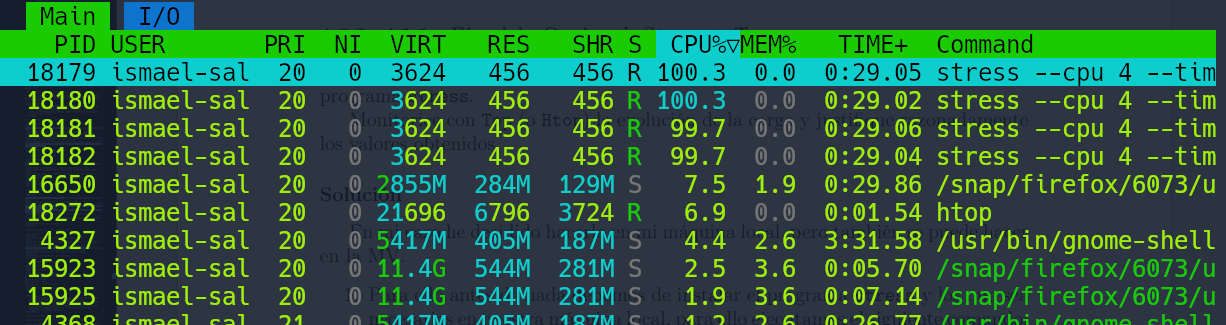
\includegraphics[width=0.6\textwidth]{images/Bloque2/htop.png}
        \caption{Ejecución del comando stress y monitorización con top}
        \label{fig:stress-top}
    \end{figure}

    \subsubsection*{Justificación razonada de los resultados}

    \paragraph{Carga del sistema (load average):}
    El valor de \textit{load average} refleja el número de procesos que están esperando utilizar la CPU. Al ejecutar el comando \texttt{stress --cpu 4}, el \textit{load average} aumentó hasta aproximadamente 4.00 en el intervalo de 1 minuto. Este valor es consistente con el número de núcleos disponibles en el sistema (4). Si el \textit{load average} hubiera superado el número de núcleos, habría indicado una sobrecarga del sistema.

    \paragraph{Uso de CPU:}
    Cada hilo generado por \texttt{stress} consumió un núcleo al 100\%. Esto se verificó mediante la herramienta \texttt{htop}, que mostró 4 procesos \texttt{stress} activos, cada uno utilizando entre el 99\% y el 100\% de la CPU. Este comportamiento confirma que los núcleos estaban completamente ocupados procesando las tareas generadas por \texttt{stress}.

    \paragraph{Uso de RAM:}
    En esta prueba no se utilizó la opción \texttt{--vm}, por lo que no se observó un uso significativo de memoria RAM. Si se hubiera incluido esta opción, la memoria libre habría disminuido proporcionalmente a la cantidad solicitada por cada hilo, lo que podría haber afectado al rendimiento general del sistema.

    \paragraph{Comportamiento general:}
    El sistema no mostró síntomas de ralentización significativa durante la prueba, lo que indica que la carga generada por \texttt{stress} fue manejada adecuadamente por los recursos disponibles. Esto demuestra que el sistema respondió de manera eficiente a las tareas intensivas generadas artificialmente, manteniendo un comportamiento estable bajo la carga simulada.



\end{enumerate}

\section{Programación de tareas periódicas con cron}

\subsection*{Tareas Periódicas en Administración de Servidores}

En la administración de servidores, es habitual automatizar tareas de mantenimiento que se repiten con cierta frecuencia. Estas tareas incluyen la verificación del estado del sistema, la rotación de archivos de registro y la limpieza de recursos. De igual forma, en procesos de monitorización, se suelen programar ejecuciones periódicas para recolectar información del sistema.

Aunque existen herramientas modernas que permiten una gestión más avanzada de estas tareas, muchas administraciones siguen utilizando herramientas tradicionales debido a su simplicidad, compatibilidad y extensa adopción en distintos entornos.

\subsection{Ejercicio Opcional. Tarea periódica con cron}

Empleando \texttt{cron} y la utilidad \texttt{logger}, programe una tarea periódica en su espacio de usuario que genere un mensaje de log con la etiqueta \texttt{ISE} y cuyo texto tenga la forma:

\begin{center}
\texttt{<SusIniciales>: <Fecha y hora actual> – <Carga actual del Sistema>}
\end{center}

\subsection*{Solución}

Es simple, tan solo debemos de:
\begin{enumerate}
    \item Crear un script con el código que se encuentra en el fichero del repositorio.
    \item Dar permisos de ejecución al script.
    \item Ejecutar el comando \texttt{crontab -e} para editar el archivo de configuración de cron.
    \item Añadir la siguiente línea al final del archivo:
    \begin{lstlisting}[style=customstyle]   
* * * * * /ruta/al/script.sh
    \end{lstlisting}
    \item Guardar y salir del editor.
    \item Verficamos usando el comando \texttt{journalctl -t ISE} que se han generado los logs.
    \item Comprobar los logs generados en el archivo de log especificado en el script.
\end{enumerate}

\section{Logs del sistema}

Una forma básica de monitorización consiste en analizar los registros (\textit{logs}) generados por el sistema operativo y los servicios instalados. En sistemas Linux, estos logs se almacenan en el directorio \texttt{/var/log}, el cual contiene tanto registros del propio sistema (como \texttt{messages}, \texttt{secure}, \texttt{lastlog}, \texttt{btmp}, entre otros) como de servicios adicionales, por ejemplo servidores web.

Muchos de estos archivos están en formato de texto plano, lo que permite su visualización mediante comandos comunes como \texttt{cat}, \texttt{grep}, \texttt{less}, \texttt{more} o \texttt{tail}. Es común encontrar múltiples versiones de un mismo log, como \texttt{cron}, \texttt{cron-20240222}, \texttt{cron-20240225}, etc. Estas versiones corresponden a rotaciones del archivo original, las cuales permiten mantener el tamaño de los logs en niveles razonables para facilitar su lectura y gestión.

La herramienta responsable de esta rotación es \texttt{logrotate}, que normalmente se ejecuta como una tarea periódica definida en \texttt{cron}. Entre sus funcionalidades se incluyen la rotación basada en tamaño o antigüedad, la compresión de logs rotados y la ejecución de acciones tras la rotación, como notificar a un servicio.

La configuración general de \texttt{logrotate} se encuentra en \texttt{/etc/logrotate.conf}, mientras que las configuraciones específicas por servicio están en \texttt{/etc/logrotate.d/}. Además, algunos servicios como Apache incluyen utilidades propias para la rotación, como \texttt{rotatelogs}, la cual permite la gestión de logs sin necesidad de reiniciar el servicio y es fácil de integrar con aplicaciones que escriben en la salida estándar.

Cabe mencionar que ciertos logs están en formato binario y requieren comandos específicos para su consulta, como \texttt{last} o \texttt{who} para los archivos \texttt{btmp} y \texttt{wtmp}.

Finalmente, el sistema \texttt{systemd} centraliza la gestión de logs mediante el servicio \texttt{systemd-journald}. Por defecto, este servicio almacena los logs de manera volátil, pero es posible habilitar su persistencia creando el directorio \texttt{/var/log/journal}. Para visualizar estos registros, se utiliza el comando \texttt{journalctl}.

\subsection{Ejercicio Opcional. Logs de arranque del sistema}

Consulte los logs del último arranque de una MV Rocky empleando \texttt{journalctl}. Concretamente, presente mensajes de niveles \texttt{warning} o más importantes.

\section*{Consulta de Logs de Arranque con \texttt{journalctl}}

El objetivo de este ejercicio es consultar los registros del sistema generados durante el último arranque de una máquina virtual Rocky Linux, utilizando la herramienta \texttt{journalctl}, y filtrar únicamente aquellos mensajes cuyo nivel de prioridad sea \texttt{warning} o superior.

\subsection*{Paso 1: Acceder al sistema}

Abra una terminal en la máquina virtual Rocky Linux, ya sea de forma local o mediante acceso remoto (por ejemplo, SSH).

\subsection*{Paso 2: Verificar el servicio \texttt{systemd-journald}}

Antes de consultar los registros, asegúrese de que el servicio de registro del sistema se encuentra en ejecución. Para ello, ejecute el siguiente comando:

\begin{verbatim}
systemctl status systemd-journald
\end{verbatim}

El resultado debe indicar que el servicio está activo y en ejecución (\texttt{active (running)}).

\subsection*{Paso 3: Consultar los logs del último arranque}

Para obtener únicamente los mensajes correspondientes al último arranque del sistema y cuyo nivel de prioridad sea \texttt{warning} o más grave, utilice el siguiente comando:

\begin{verbatim}
journalctl -b -p warning
\end{verbatim}

Este comando muestra los mensajes generados desde el último arranque con prioridad \texttt{warning}, \texttt{err}, \texttt{crit}, \texttt{alert} o \texttt{emerg}.

\subsection*{Paso 4: Visualización y exportación de los logs (opcional)}

Si desea navegar por los mensajes de manera más cómoda, puede usar un paginador como \texttt{less}:

\begin{verbatim}
journalctl -b -p warning | less
\end{verbatim}

Para guardar los registros en un archivo de texto, use la redirección de salida:

\begin{verbatim}
journalctl -b -p warning > logs_arranque.txt
\end{verbatim}

\subsection*{Paso 5: Consultar arranques anteriores (opcional)}

En caso de querer revisar los logs de un arranque anterior al actual, utilice la opción \texttt{-b -1}, como se muestra a continuación:

\begin{verbatim}
journalctl -b -1 -p warning
\end{verbatim}

\subsection*{Resultado esperado}

La salida del comando debe contener mensajes con advertencias, errores o alertas que hayan ocurrido durante el arranque del sistema, lo cual permite al administrador identificar posibles incidencias o configuraciones incorrectas.

\newpage
\section{Grafana + Prometheus}

Grafana es una herramienta de código abierto orientada a la observabilidad y monitorización de sistemas. Su arquitectura se basa en componentes como los \textit{dashboards}, los paneles y las alertas, permitiendo construir una pila de observabilidad personalizada para distintos entornos. Esta herramienta ofrece opciones tanto de despliegue autogestionado como de servicio en la nube, adaptándose así a diferentes presupuestos y necesidades organizativas.

Grafana proporciona funcionalidades avanzadas de visualización y definición de alertas sobre datos de telemetría. Sin embargo, no se encarga directamente de la recolección ni del almacenamiento de estos datos. Para ello, se emplea Prometheus, una solución específicamente diseñada para extraer, almacenar y gestionar información de monitorización de manera eficiente.

Prometheus destaca por su capacidad para manejar series temporales, su modelo de datos abierto y flexible, y por soportar métricas estandarizadas. Aunque incluye funciones básicas de visualización y gestión de alertas, estas son limitadas, por lo que suele combinarse con Grafana para conformar una solución más completa. Esta combinación es ampliamente utilizada en infraestructuras tecnológicas modernas.

Ambos servicios pueden instalarse localmente en una máquina virtual Rocky Linux o en el sistema anfitrión, siempre que sea compatible. Sin embargo, para entornos de práctica o desarrollo, se recomienda su ejecución mediante contenedores Docker utilizando \texttt{docker-compose}.

\subsection*{Despliegue con Docker Compose}

Para iniciar los servicios de Prometheus y Grafana en contenedores Docker, se requiere crear un directorio (por ejemplo, \texttt{progra}) y dentro de él, definir los siguientes archivos:

\subsubsection*{Archivo \texttt{docker-compose.yml}}

\begin{verbatim}
version: "3"
services:
  prometheus:
    image: prom/prometheus:v2.50.0
    ports:
      - 9090:9090
    volumes:
      - ./prometheus_data:/prometheus
      - ./prometheus.yml:/etc/prometheus/prometheus.yml
    command:
      - "--config.file=/etc/prometheus/prometheus.yml"

  grafana:
    image: grafana/grafana:9.1.0
    ports:
      - 4000:3000
    volumes:
      - ./grafana_data:/var/lib/grafana
    depends_on:
      - prometheus
\end{verbatim}

\subsubsection*{Archivo \texttt{prometheus.yml}}

\begin{verbatim}
global:
  scrape_interval: 5s

scrape_configs:
  - job_name: "prometheus_service"
    static_configs:
      - targets: ["prometheus:9090"]
\end{verbatim}

\subsection*{Acceso a las interfaces web}

Una vez iniciados los servicios, se puede acceder a las interfaces web mediante un navegador en el equipo donde se ejecuta Docker. Prometheus estará disponible en el puerto \texttt{9090} y Grafana en el \texttt{4000}, por ejemplo: \texttt{http://localhost:9090} y \texttt{http://localhost:4000}.

\subsection*{Integración entre Grafana y Prometheus}

Para completar la integración, es necesario definir Prometheus como fuente de datos (\textit{Datasource}) en Grafana. En entornos gestionados con Docker Compose, los servicios pueden comunicarse empleando el nombre del contenedor como dominio. Por tanto, en Grafana se debe configurar la URL del datasource como \texttt{http://prometheus:9090}.

\subsection{Ejercicio Obligatorio. Monitorización con Grafana + Prometheus}

\textbf{Monitorización de Servidor Linux}

Emplear la plataforma Prometheus + Grafana instalada para monitorizar las prestaciones de un servidor Rocky corriendo en una VM. El alumno/a puede elegir los componentes de Prometheus y Grafana que prefiera o crear nuevos componentes por sí mismo/a. No obstante, se sugiere emplear como base el exporter de Linux para Prometheus\footnote{\url{https://prometheus.io/docs/guides/node-exporter/}}, configurado como un servicio\footnote{\url{https://prometheus.io/docs/prometheus/latest/getting_started/}} y emplear como base algún dashboard predefinido para Grafana\footnote{\url{https://grafana.com/grafana/dashboards}}. Siga las instrucciones de cada dashboard para posibles ajustes en Prometheus. En Grafana vaya a \texttt{Dashboards → Import} y proporcione el Id del dashboard.

El dashboard debe recibir como identificador, el nombre y apellidos del alumno/a en CamelCase junto con el sufijo “Linux”. Por ejemplo, \texttt{mariaGarciaPerezLinux}. Todos los paneles creados se presentarán con un título que contenga las iniciales del alumno/a. Siguiendo con el ejemplo anterior: \%CPU (MGP).

El alumno/a debe extender el dashboard anterior para incorporar indicadores sobre el nivel de activación (“Activo”/”Inactivo”, 1/0) de los servicios: \texttt{SSHD} y \texttt{Apache Httpd} en el equipo Linux monitorizado.

Además, deberá agregar un nuevo panel sobre el nivel de uso total de la CPU en tanto por ciento (\%). A este panel se le asociará una alarma para que se dispare cuando la media del uso de CPU supere el 75\% de CPU durante 5 minutos. Ponga de manifiesto el funcionamiento de la alarma empleando alguna herramienta de carga de las vistas en clase (por ejemplo, \texttt{stress}).

Para poner de manifiesto el funcionamiento de la monitorización, se adjuntará una memoria en la que se presenten:
\begin{itemize}
    \item Descripción de la secuencia de pasos realizada para ejecutar el exporter de Linux. Con capturas de pantalla de los pasos seguidos para su ejecución y/o configuración.
    \item Capturas de pantalla de los monitores de \texttt{Sshd} y \texttt{Httpd} poniendo de manifiesto su comportamiento cuando los servicios están activos e inactivos.
    \item Captura de pantalla del monitor de uso de CPU antes y después de lanzar la carga de CPU.
    \item Captura de pantalla del comando empleado para disparar la carga de CPU.
    \item Captura de pantalla que ponga de manifiesto el disparo de la alarma asociada al monitor de CPU.
\end{itemize}

\textbf{Monitorización de API WEB}

La aplicación empleada en el apartado anterior para la prueba de carga, expone en el path \texttt{/metrics} los indicadores de NodeJS para Prometheus. Para más información, el exporter de Prometheus de la API Web se ha generado empleando los componentes estándar: \texttt{prom-client}\footnote{\url{https://github.com/siimon/prom-client}} y \texttt{express-prom-bundle}\footnote{\url{https://github.com/jochen-schweizer/express-prom-bundle}}.

Cree un nuevo Dashboard con algunas de las métricas expuestas. Para el dashboard emplee como nombre su nombre y apellidos en CamelCase seguido del sufijo API. Por ejemplo, \texttt{anaTorrentRamonetAPI}. Todos los paneles creados se presentarán con un título que contenga las iniciales del alumno/a. Siguiendo con el ejemplo anterior: \%Memoria (ATR).

Cree monitores para las siguientes métricas:
\begin{itemize}
    \item Tiempos de respuesta de los endpoints de la API (\texttt{http\_request\_duration\_seconds\_bucket}).
    \item Memoria disponible (\texttt{nodejs\_heap\_size\_total\_bytes}) vs la usada actualmente (\texttt{nodejs\_heap\_size\_used\_bytes}).
    \item Uso de CPU (\texttt{process\_cpu\_seconds\_total}).
\end{itemize}

Realice una memoria de prácticas en la que se ponga de manifiesto la ejecución de la prueba de carga diseñada para JMeter y se aprecie el efecto de la misma en los monitores anteriormente descritos.

\textbf{Entregables para este ejercicio:}
\begin{itemize}
    \item Memoria en formato PDF con las capturas solicitadas en la monitorización del servidor Linux.
    \item Memoria en formato PDF con las capturas solicitadas en la monitorización de la API web.
    \item Configuración de scraping de Prometheus (vista en \texttt{prometheus.yaml}).
    \item Definición de los dos dashboards de Grafana. Para esto último, debe emplear la opción de \texttt{Share Dashboard or Panel} y exportar el Dashboard con la opción \texttt{Export for sharing externally}.
\end{itemize}

\begin{figure}[H]
    \centering
    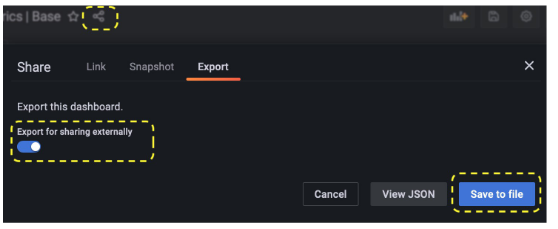
\includegraphics[width=0.6\textwidth]{images/Bloque2/enunciado_grafana.png}
    \label{fig:grafana}
\end{figure}

\subsection*{Solución}

\begin{enumerate}
    \item Primer paso:
    \begin{figure}[H]
        \centering
        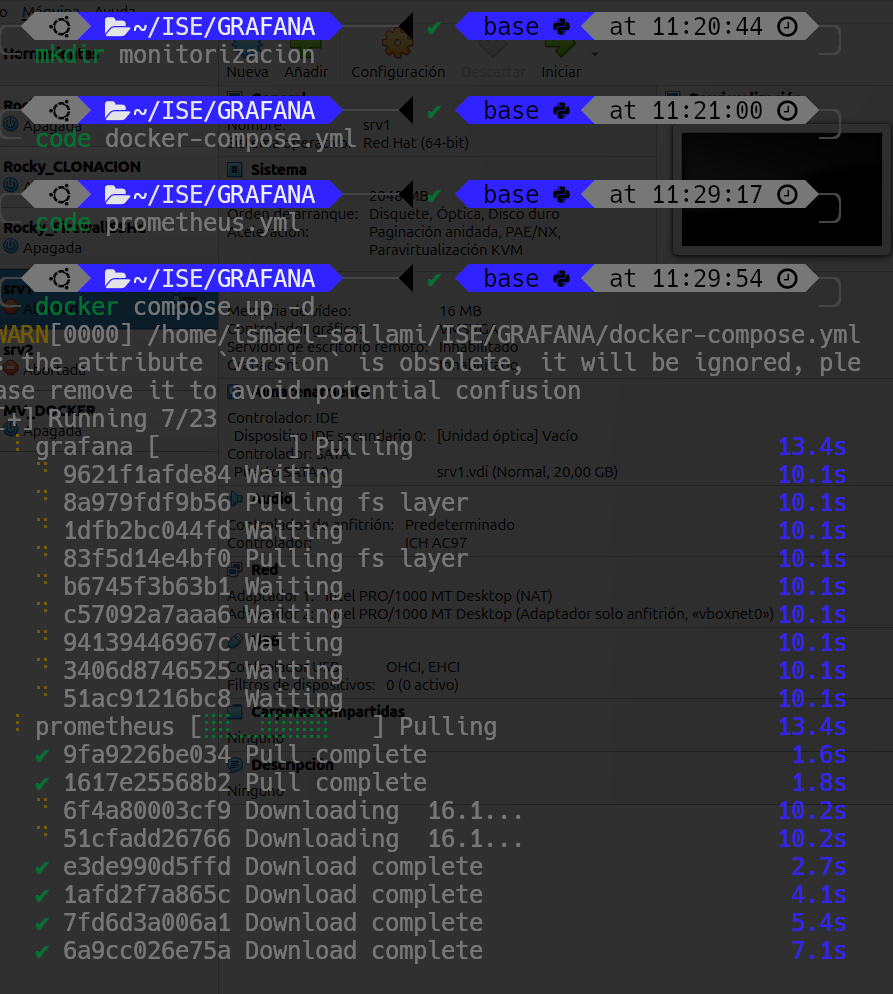
\includegraphics[width=0.6\textwidth]{images/Bloque2/graf1.png}
        \caption{Creación del directorio y descarga de los archivos necesarios}
        \label{fig:instalacion}
    \end{figure}
    \item Clonamos una máquina virtual Rocky Linux. En mi caso le he cambiado la IP y a continuación voy a hacer ssh para hacerlo desde mi máquina local y que me sea más cómodo.
    \item Dentro de la MV Rocky Linux:
    \begin{enumerate}
        \item Primer paso nos bajamos el node-exporter de Prometheus:
        \begin{figure}[H]
            \centering
            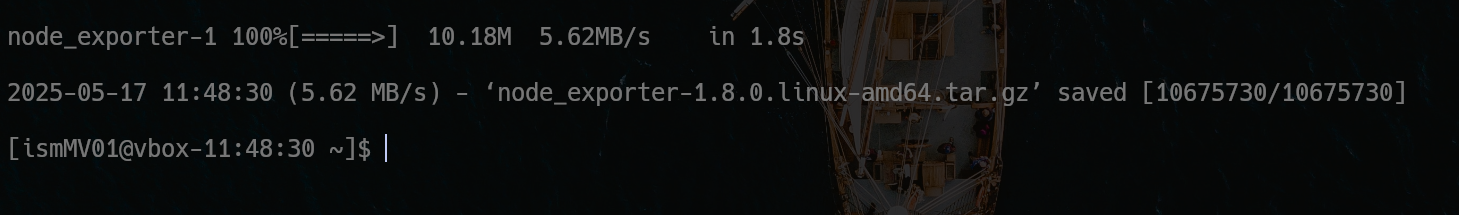
\includegraphics[width=0.6\textwidth]{images/Bloque2/graf2.png}
            \caption{Descarga del node-exporter}
            \label{fig:node-exporter}
        \end{figure}
        \item Descomprimimos el archivo\footnote{He tenido que instalar los comandos tar y wget.}:
        \begin{figure}[H]
            \centering
            \includegraphics[width=0.6\textwidth]{images/Bloque2/graf3.png}
            \caption{Descompresión del node-exporter}
            \label{fig:descompresion}
        \end{figure}
        \item Movemos el binario al directorio del sistema:
        \begin{figure}[H]
            \centering
            \includegraphics[width=0.6\textwidth]{images/Bloque2/graf4.png}
            \caption{Movimiento del binario al directorio del sistema}
            \label{fig:movimiento}
        \end{figure}
        \item Verificamos que funciona:
        \begin{figure}[H]
            \centering
            \includegraphics[width=0.6\textwidth]{images/Bloque2/graf5.png}
            \caption{Verificación del funcionamiento del node-exporter}
            \label{fig:verificacion}
        \end{figure}
        \item Creamos el usuario:
        \begin{figure}[H]
            \centering
            \includegraphics[width=0.6\textwidth]{images/Bloque2/graf6.png}
            \caption{Creación del usuario}
            \label{fig:usuario}
        \end{figure}
        \item Creamos el servicio:
        \begin{figure}[H]
            \centering
            \includegraphics[width=0.6\textwidth]{images/Bloque2/graf7.png}
            \caption{Creación del servicio}
            \label{fig:servicio}
        \end{figure}
        El contenido del archivo \texttt{node-exporter.service} es el siguiente:
        \begin{lstlisting}[style=customstyle]
            [Unit]
            Description=Node Exporter
            After=network.target

            [Service]
            User=node_exporter
            Group=node_exporter
            Type=simple
            ExecStart=/usr/local/bin/node_exporter

            [Install]
            WantedBy=multi-user.target
        \end{lstlisting}
        \item Recargamos, habilitams y reiniciamos el servicio:
        \begin{figure}[H]
            \centering
            \includegraphics[width=0.6\textwidth]{images/Bloque2/graf8.png}
            \caption{Recarga, habilitación y reinicio del servicio}
            \label{fig:recarga}
        \end{figure}

        \textbf{Se supone que el servicio debería de estar activo, pero me daba un error.} Tras un tiempo intentando arreglarlo, el error se debía a que el servicio node\_exporter fallaba al iniciar debido a una política de SELinux que denegaba su ejecución. Se solucionó corrigiendo el contexto de seguridad SELinux del binario /usr/local/bin/node\_exporter al tipo bin\_t.

        \item Ahora podemos ver que el servicio está activo:
        \begin{figure}[H]
            \centering
            \includegraphics[width=0.6\textwidth]{images/Bloque2/graf9.png}
            \caption{Verificación del servicio}
            \label{fig:verificacion_servicio}
        \end{figure}
        \item Ahora debemos de ver si Node Exporter expone métricas por red, para ello debemos de ejecutar el comando: \micode{curl http://localhost:9100/metrics} en la máquina virtual.
        \begin{figure}[H]
            \centering
            \includegraphics[width=0.6\textwidth]{images/Bloque2/graf10.png}
            \caption{Verificación de las métricas expuestas tras la ejecución del comando}
            \label{fig:metricas}
        \end{figure}
        \item Ahora si accedemos desde nuestra máquina local a la dirección \micode{http://<IP\_VM>:9100/metrics} podemos ver las métricas expuestas por el node-exporter, pero antes debemos de verificar el firewall:
        \begin{figure}[H]
            \centering
            \includegraphics[width=0.6\textwidth]{images/Bloque2/graf11.png}
            \caption{Verificación del firewall}
            \label{fig:firewall}
        \end{figure}
        \item Ahora si accedemos desde nuestra máquina local a la dirección \micode{http://<IP\_VM>:9100/metrics} podemos ver las métricas expuestas por el node-exporter:
        \begin{figure}[H]
            \centering
            \includegraphics[width=0.6\textwidth]{images/Bloque2/graf12.png}
            \caption{Acceso a las métricas expuestas}
            \label{fig:acceso_metricas}
        \end{figure}

    \end{enumerate}
    \item Ahora debemos de configurar Prometheus para recolectar Métricas de Node Exporter\footnote{Esto lo haremos en nuestra máquina local.}. Para ello debemos de editar el archivo \texttt{prometheus.yml} y añadir el siguiente bloque de configuración:
    \begin{lstlisting}[style=customstyle]
        - job_name: 'rocky_linux_server'
        static_configs:
        - targets: ['192.168.56.102:9100'] 
    \end{lstlisting}
    \item Reiniciamos el contenedor de Prometheus para que recoja la nueva configuración:
    \begin{figure}[H]
        \centering
        \includegraphics[width=0.6\textwidth]{images/Bloque2/graf13.png}
        \caption{Reinicio del contenedor de Prometheus}
        \label{fig:reinicio}
    \end{figure}
    \textbf{Nota:} Al iniciar los contendores me daba un problema de permisos, por ende, tuve que ejecutar los comandos: 
    \begin{lstlisting}[style=customstyle]
        Para Prometheus:
        Bash

        mkdir -p ./prometheus_data
        sudo chown -R 65534:65534 ./prometheus_data
        sudo chmod -R 755 ./prometheus_data

        Para Grafana:
        Bash

        mkdir -p ./grafana_data
        sudo chown -R 472:472 ./grafana_data
        sudo chmod -R 755 ./grafana_data
    \end{lstlisting}

    Vemos que los contenedores están activos:
    \begin{figure}[H]
        \centering
        \includegraphics[width=0.6\textwidth]{images/Bloque2/graf14.png}
        \caption{Contenedores activos}
        \label{fig:contenedores}
    \end{figure}
    \item Ahora accedemos a la interfaz web de Prometheus en \micode{http://localhost:9090}:
    \begin{figure}[H]
        \centering
        \includegraphics[width=0.6\textwidth]{images/Bloque2/graf15.png}
        \caption{Interfaz web de Prometheus}
        \label{fig:interfaz_prometheus}
    \end{figure}
    \item Vemos que en targets tenemos el Rocky Linux:
    \begin{figure}[H]
        \centering
        \includegraphics[width=0.6\textwidth]{images/Bloque2/graf16.png}
        \caption{Targets de Prometheus}
        \label{fig:targets}
    \end{figure}
    Vemos que efectivamente está activo ya que el estado es UP.
    \item Ahora accedemos a la interfaz web de Grafana en \micode{http://localhost:4000}:
    \begin{figure}[H]
        \centering
        \includegraphics[width=0.6\textwidth]{images/Bloque2/graf17.png}
        \caption{Interfaz web de Grafana}
        \label{fig:interfaz_grafana}
    \end{figure}
    Al ser nuevos, accedemos con el usuario admin y la contraseña admin. Nos pedirá que cambiemos la contraseña, así que la cambiamos.
    \item Ahora debemos de añadir la fuente de datos, para ello vamos a \texttt{Configuration $\rightarrow$ Data Sources $\rightarrow$ Add data source} y seleccionamos Prometheus:
    \begin{figure}[H]
        \centering
        \includegraphics[width=0.6\textwidth]{images/Bloque2/graf18.png}
        \caption{Añadir fuente de datos}
        \label{fig:fuente_datos}
    \end{figure}
    \item Importamos un dashboard de Grafana, para ello vamos a \texttt{Dashboards $\rightarrow$ Import} y buscamos el ID del dashboard que queremos importar. En mi caso he elegido el ID 1860\footnote{\url{https://grafana.com/grafana/dashboards/1860}}:
    \begin{figure}[H]
        \centering
        \includegraphics[width=0.6\textwidth]{images/Bloque2/graf19.png}
        \caption{Importación del dashboard}
        \label{fig:importacion_dashboard}
    \end{figure}
    \item Ahora debemos de añadir las iniciales a los paneles, quedando de esta manera(las iniciales son ISM):
    \begin{figure}[H]
        \centering
        \includegraphics[width=0.6\textwidth]{images/Bloque2/graf20.png}
        \caption{Añadido de las iniciales a los paneles}
        \label{fig:iniciales_paneles}
    \end{figure} 
    Siguiendo con el enunciado vamos a responder a la parte de:
    ``El dashboard debe recibir como identificador, el nombre y apellidos del alumno/a en CamelCase
    junto con el sufijo “Linux”. Por ejemplo, mariaGarciaPerezLinux. Todos los paneles creados se
    presentarán con un título que contenga las iniciales del alumno/a. Siguiendo con el ejemplo
    anterior: \%CPU (MGP).''
    De manera que el dashboard quedaría de la siguiente manera:
    \begin{figure}[H]
        \centering
        \includegraphics[width=0.6\textwidth]{images/Bloque2/graf21.png}
        \caption{Dashboard con el nombre y apellidos del alumno}
        \label{fig:dashboard}
    \end{figure}
    Como vemos en la imagen el dashboard tiene el nombre y apellidos del alumno/a en CamelCase junto con el sufijo “Linux” y todos los paneles creados se presentan con un título que contiene las iniciales del alumno/a (esto se omite ya que al ser un dashboard predefinido tiene varios paneles y es muy costoso ir cambiando todos los nombres de los paneles).
    \item Añadimos un nuevo panel en este dashboard que hemos creado con nuestro nombre:
    \begin{figure}[H]
        \centering
        \includegraphics[width=0.6\textwidth]{images/Bloque2/graf22.png}
        \caption{Añadido de un nuevo panel}
        \label{fig:nuevo_panel}
    \end{figure}
    Al añadir el panel del ssh no me daba los valores correctos, así que probé a poner la métrica en el prometheus y tampoco me daba resultado, por ende añadí al fichero \texttt{/etc/systemd/system/node\_exporter.service}
    a la línea de ``exec'' la parte de \micode{--collector.systemd} y recargando toda la configuración sí me da el resultado correcto. Nos quedaría de la siguiente manera:
    \begin{figure}[H]
        \centering
        \includegraphics[width=0.6\textwidth]{images/Bloque2/graf23.png}
        \caption{Añadido del panel del ssh}
        \label{fig:panel_ssh}
    \end{figure}

    \item Ahora debemos de hacer lo mismo para httpd:
    \begin{figure}[H]
        \centering
        \includegraphics[width=0.6\textwidth]{images/Bloque2/graf24.png}
        \caption{Añadido del panel del httpd}
        \label{fig:panel_httpd}
    \end{figure}

    De manera conjunta nos quedaría de la siguiente manera:
    \begin{figure}[H]
        \centering
        \includegraphics[width=0.6\textwidth]{images/Bloque2/graf25.png}
        \caption{Añadido de los paneles del ssh y httpd}
        \label{fig:paneles_ssh_httpd}
    \end{figure}
    \textbf{Nota:} Las expresiones regulares que he utilizado para el ssh y httpd aparecen en las imágenes de arriba.
    \item Ahora añadimos el panel de la CPU:
    \begin{figure}[H]
        \centering
        \includegraphics[width=0.6\textwidth]{images/Bloque2/graf26.png}
        \caption{Añadido del panel de la CPU}
        \label{fig:panel_cpu}
    \end{figure}

    \item Ahora añadimos la alarma al panel de la CPU:
    \begin{figure}[H]
        \centering
        \begin{minipage}{0.45\textwidth}
            \centering
            \includegraphics[width=\textwidth]{images/Bloque2/graf27.png} % Llave añadida
            \caption{Primera Parte de la alarma}
            \label{fig:image1graf}
        \end{minipage}
        \hfill
        \begin{minipage}{0.45\textwidth}
            \centering
            \includegraphics[width=\textwidth]{images/Bloque2/graf28.png}
            \caption{Segunda Parte de la alarma}
            \label{fig:image2graf}
        \end{minipage}
    \end{figure}
    \item De manera que la alarma nos quedaría de la siguiente manera:
    \begin{figure}[H]
        \centering
        \includegraphics[width=0.6\textwidth]{images/Bloque2/graf29.png}
        \caption{Alarma de la CPU}
        \label{fig:alarma_cpu}
    \end{figure}
    \item Ahora vamos a ver el estado incial y el estado final de la CPU.
    \begin{figure}[H]
        \centering
        \includegraphics[width=0.6\textwidth]{images/Bloque2/graf30.png}
        \caption{Estado inicial de la CPU}
        \label{fig:estado_inicial_cpu}
    \end{figure}

    Para instalar el stress en la máquina virtual de Rocky Linux, ejecutamos el siguiente comando:
    \begin{lstlisting}[style=customstyle]
    sudo dnf install epel-release -y
    sudo dnf makecache
    sudo dnf install stress -y
    \end{lstlisting}

    Vemos que si ejecutamos el comando \micode{stress --cpu 1 --timeout 360s} la carga en grafana va a subir poco a poco y cuando supere el 75\% de CPU durante 5 minutos se disparará la alarma:
    \begin{figure}[H]
        \centering
        \begin{minipage}{0.45\textwidth}
            \centering
            \includegraphics[width=\textwidth]{images/Bloque2/graf31.png}
            \caption{Alto uso de CPU gracias al stress}
            \label{fig:image1}
        \end{minipage}
        \hfill
        \begin{minipage}{0.45\textwidth}
            \centering
            \includegraphics[width=\textwidth]{images/Bloque2/graf33.png}
            \caption{Disparo de la alarma}
            \label{fig:image2}
        \end{minipage}
    \end{figure}

    Luego al cancelar el stress, la carga de CPU baja y la alarma se apaga:
    \begin{figure}[H]
        \centering
        \begin{minipage}{0.45\textwidth}
            \centering
            \includegraphics[width=\textwidth]{images/Bloque2/graf32.png}
            \caption{Vuelta al uso normal de CPU}
            \label{fig:image1}
        \end{minipage}
        \hfill
        \begin{minipage}{0.45\textwidth}
            \centering
            \includegraphics[width=\textwidth]{images/Bloque2/graf34.png}
            \caption{Estado normal de la alarma}
            \label{fig:image2}
        \end{minipage}
    \end{figure}
    
    El comando ha sido:
    \begin{figure}[H]
        \centering
        \includegraphics[width=0.6\textwidth]{images/Bloque2/graf35.png}
        \caption{Comando de stress}
        \label{fig:comando_stress}
    \end{figure}
\end{enumerate}

\textcolor{blue}{Ahora pasamos a la parte de la resolución de la API WEB.}

Para la realización de esta parte debemos de tener en cuenta el ejercicio de prueba de carga con JMETER, para ello lanzamos el contenedor de la API Web y entramos en la url \micode{http://localhost:3000/metrics}.

Una vez añadido los paneles y demás \footnote{A continuación se adjuntan las expresiones regulares que he utilizado para cada uno de los paneles.}, vamos a ver como queda el antes y después de los paneles tras la carga de JMeter.

\begin{figure}[H]
    \centering
    \includegraphics[width=0.6\textwidth]{images/Bloque2/graf36.png}
    \caption{Paneles de la API Web Antes de la carga}
    \label{fig:paneles_api}
\end{figure}

Por último, tras la carga de JMeter, los paneles quedan de la siguiente manera:
\begin{figure}[H]
    \centering
    \includegraphics[width=0.6\textwidth]{images/Bloque2/graf37.png}
    \caption{Paneles de la API Web Después de la carga}
    \label{fig:paneles_api_despues}
\end{figure}












% Referencias
\begin{thebibliography}{99}
\bibitem{Referencia1}
Ismael Sallami Moreno, \textbf{Estudiante del Doble Grado en Ingeniería Informática + ADE}, Universidad de Granada, 2025.

\bibitem{turn0search0} Introduction to ad hoc commands - Ansible Documentation. \url{https://docs.ansible.com/ansible/latest/command_guide/intro_adhoc.html}
\bibitem{turn0search4} Index of all Modules — Ansible Community Documentation. \url{https://docs.ansible.com/ansible/latest/collections/index_module.html}
\bibitem{turn0search2} Ansible playbooks — Ansible Community Documentation. \url{https://docs.ansible.com/ansible/latest/playbook_guide/playbooks_intro.html}
% \bibitem{Referencia2}
% Autor(es), \emph{Título del libro}, Editorial, año.

% \bibitem{Referencia3}
% Autor(es), \emph{Título del documento}, Nombre de la Conferencia, páginas, año.
\end{thebibliography}



\end{document}
